\chapter{Higgs Discovery in $ZZ\rightarrow4l$}
\label{sec:discovery}
\chaptermark{Discovery}

\begin{center}
\begin{footnotesize}
\textit{\textbf{Vladimir}: That passed the time.\\
\textbf{Estragon}: It would have passed in any case.\\
\textbf{Vladimir}: Yes, but not so rapidly.}\\
Samuel Beckett, ``Waiting for Godot"
\end{footnotesize}
\end{center}

\section{Object Definitions}
\label{sec:zz4lObjects}

As specified in Sec.~\ref{sec:HiggsDecay}, $H\rightarrow ZZ \rightarrow 4l$ should be ideal for Higgs discovery. In this channel, we need four good lepton tracks for kinematic decay reconstruction, any relevant radiated photons for proper energy measurements, and a collection of any jets to examine the production of any resonance. Although rough reconstructions were defined in Sec.~\ref{sec:ParticleID}, our objects must be explicitly defined to examine the certainty of any results. To do so, we need four\footnote{Although the tau is also a lepton, it decays quickly and tends to appear more like a jet making the mass resolution of a $H\rightarrow ZZ \rightarrow 2l2\tau$ worse than a $4l$ event. For this reason, taus are not considered in the $H\rightarrow ZZ \rightarrow 4l$ analyses in this thesis.} objects: electrons, muons, photons, and jets.

\subsection{Electrons}
\label{sec:zz4lElectrons}

Electrons are geometrically constrained such that $|\eta^e|<2.5$, with a $p_T^e>7$ $\rm{GeV}$ cut is applied to maintain reasonable reconstruction efficiency while preserving capability to find low mass Higgs candidates. As referenced in Sec.~\ref{sec:ParticleID}, to reconstruct an electron, usually clusters of energy deposits in the ECAL are used as seeds to match to tracks from the silicon tracker (``outside-in" approach). However, to improve efficiency of low $p_T$ electrons, the opposite approach is also taken where trajectories are used to find clusters in the ECAL (``inside-out"). As electrons pass through the tracker volume, there will be some energy loss via bremsstrahlung which is modeled and fit using a gaussian sum filter. More details on the reconstruction algorithm is found in \cite{,,}. The expected energy resolution for prompt and isolated (see Sec.~\ref{sec:zz4lIsolation}) electrons is found in Fig.~\ref{fig:ElectronEnergyResolution}.

\begin{figure}[htbp]
\begin{center}
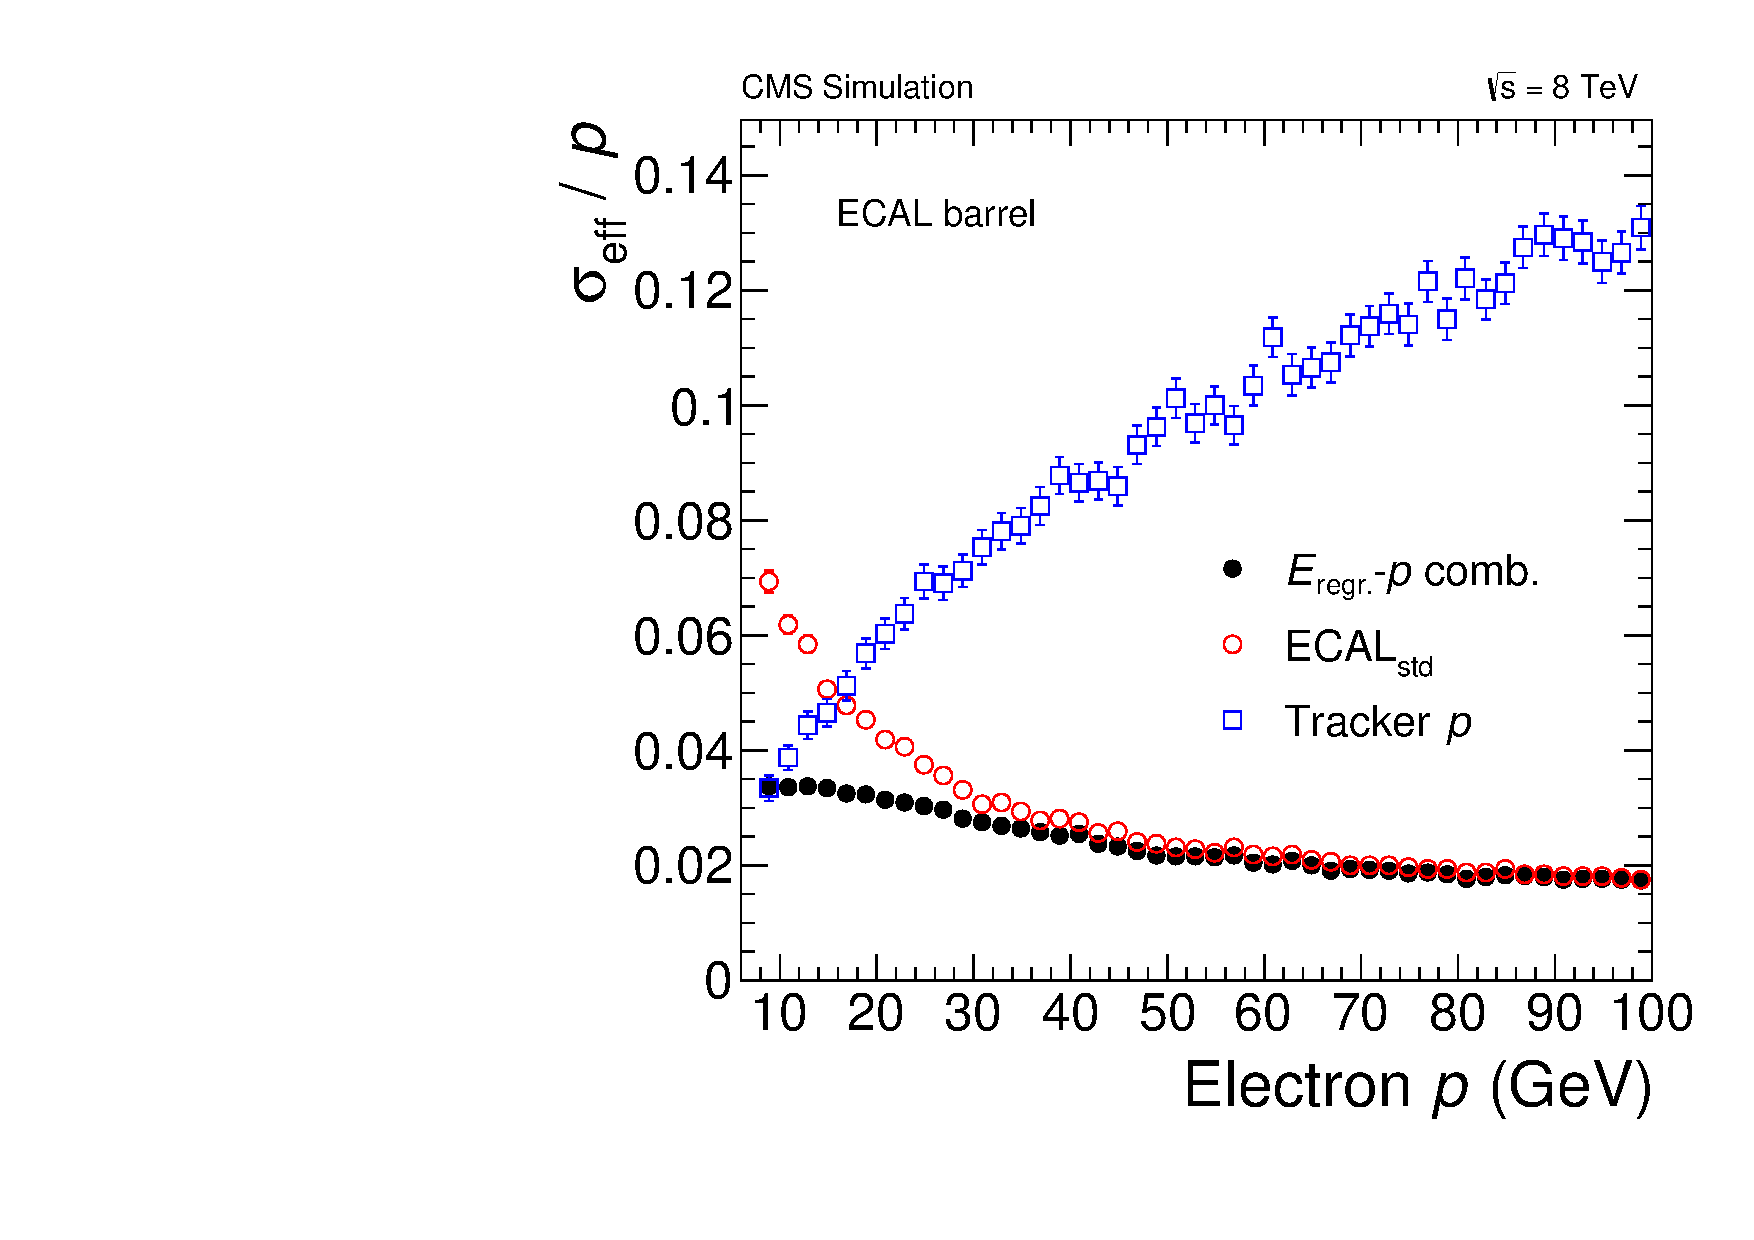
\includegraphics[width=.6\linewidth]{HiggsDiscovery/figures/effRMSbarrel_withregression_new.pdf}
\caption[Expected Energy Resolution for Electrons]{Expected energy resolution for prompt and isolated electrons in the ECAL barrel as a function of the initial energy. The effective resolution is better in the tracker (open blue squares) for low energy electrons, while the ECAL has better resolution for high energy electrons (open red circles). This encourages the use of both outside-in and inside-out techniques. The effective resolution (solid black circles) is $\lesssim 4\%$ of the initial energy. }
\label{fig:ElectronEnergyResolution}
\end{center}
\end{figure}

For identification, a Boosted Decision Tree\footnote{BDTs are a subset of the broader machine learning technique, decision tree learning, which utilizes multiple decision trees to classify data.} (BDT) multivariate technique \cite{} is trained using observables for electrons, such as the amount of energy radiated via bremsstrahlung during flight, matching between trajectories and ECAL clusters, and shower shapes in the ECAL. This method improves the resolution by $\sim 10\%$ per electron compared to cut-based techniques.

Lastly, to validate the momentum scale of the electrons in the $4l$ channel, invariant mass distributions of data from well-known SM particles that decay to $e^+e^-$ are compared to analytical distributions. In the left plot of Fig.~\ref{fig:ElectronMassResolutionAndBias}, electrons with $p_T\gtrsim35$ $\rm{GeV}$ show a bias in the reconstructed mass within $\sim0.3\%$ across three different decays\footnote{$J/\Psi$ is a meson made of $c\bar{c}$ with mass $m_{J/\Psi}=3.1$ $\rm{GeV}$ while $\Upsilon$ is a meson made of $b\bar{b}$ with mass $m_{\Upsilon}=9.6$ $\rm{GeV}$. Along with the $Z$, they have masses greater than $2m_e$ or $2m_\mu$, so they can be used as references to validate mass reconstruction.} ($Z$, $J/\Psi$, $\Upsilon$) for multiple pseudorapidity ranges. A small mass shift appears for lower $p_T$ electrons, accounted for as a systematic in the signal mass scale. The effective mass resolution in $Z\rightarrow e^+e^-$, found in  the right plot of Fig.~\ref{fig:ElectronMassResolutionAndBias}, is below $4\%$ for the full range of the ECAL.

\begin{figure}[htbp]
\begin{center}
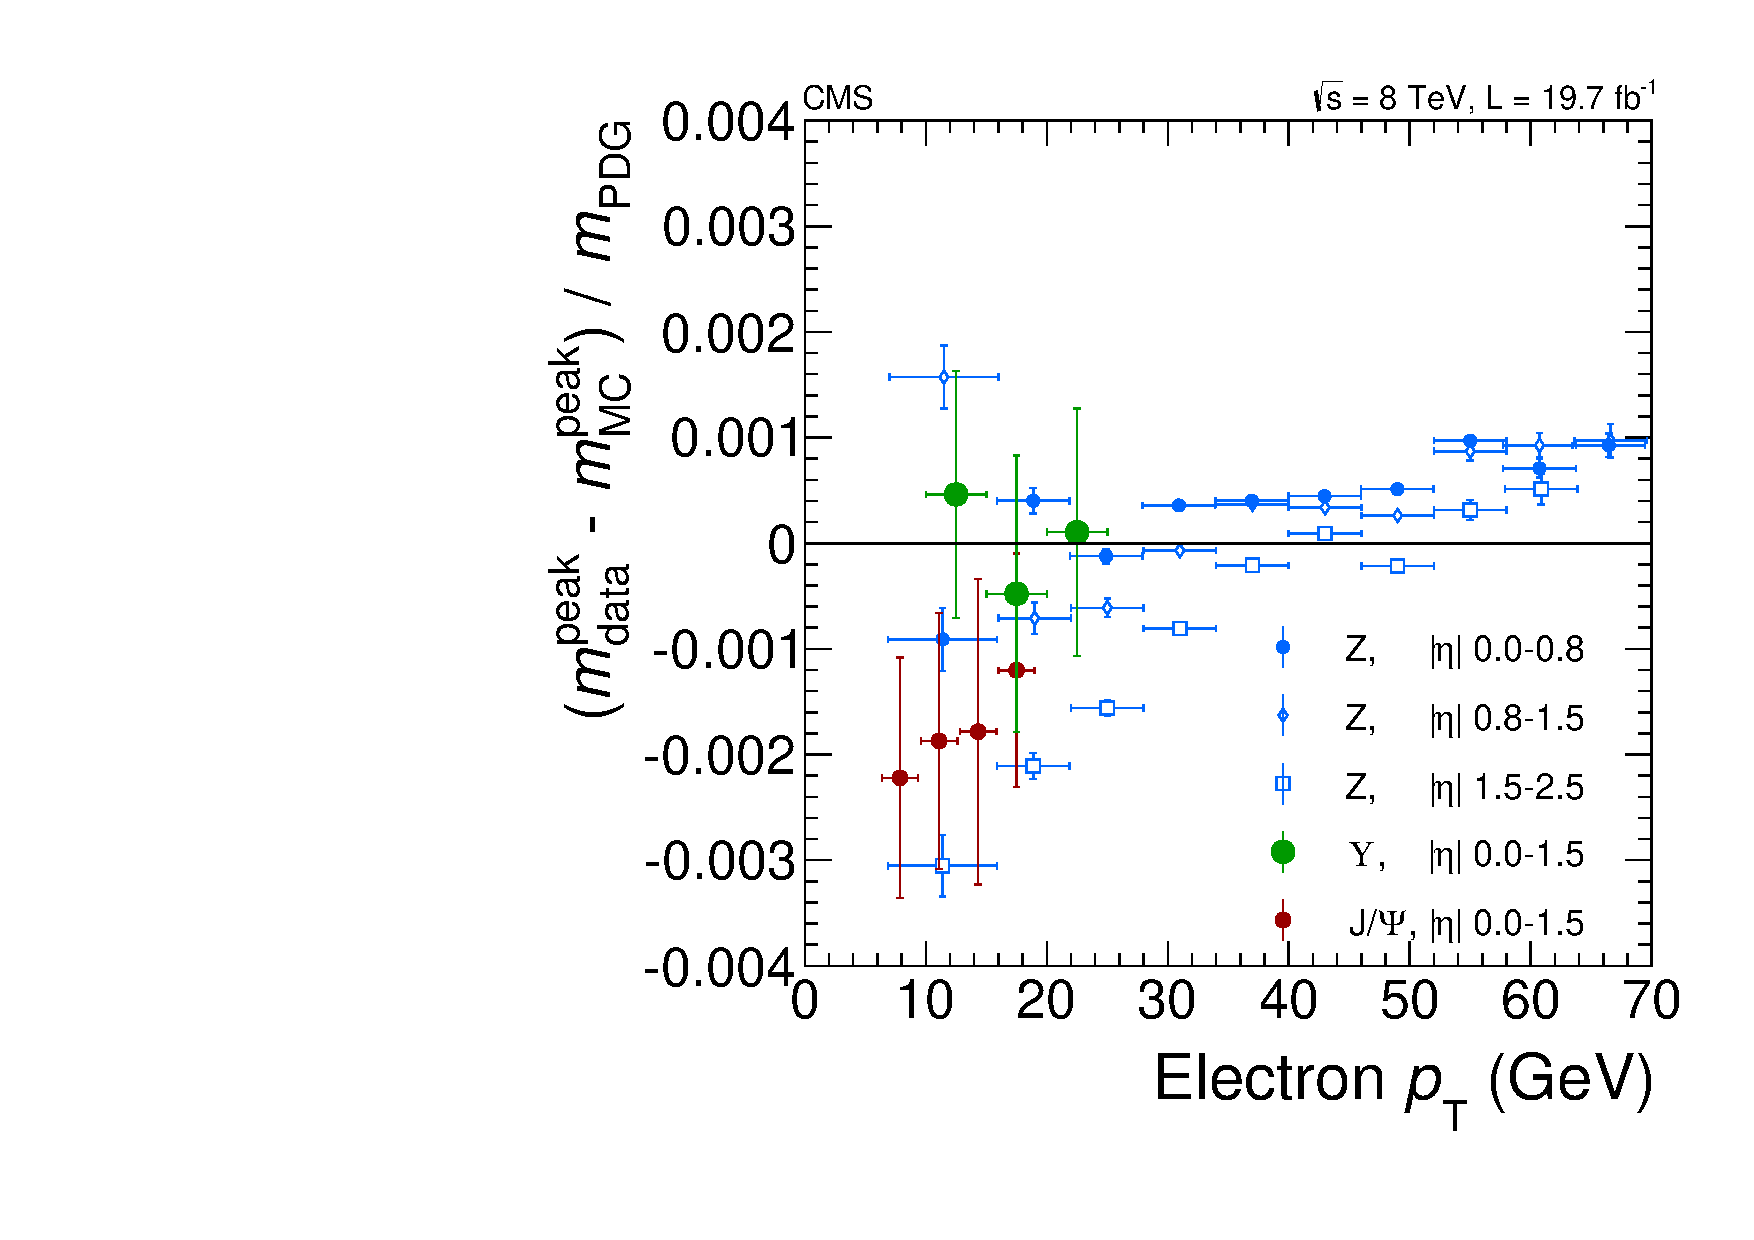
\includegraphics[width=.45\linewidth]{HiggsDiscovery/figures/scale-ptdep-8TeV.pdf}
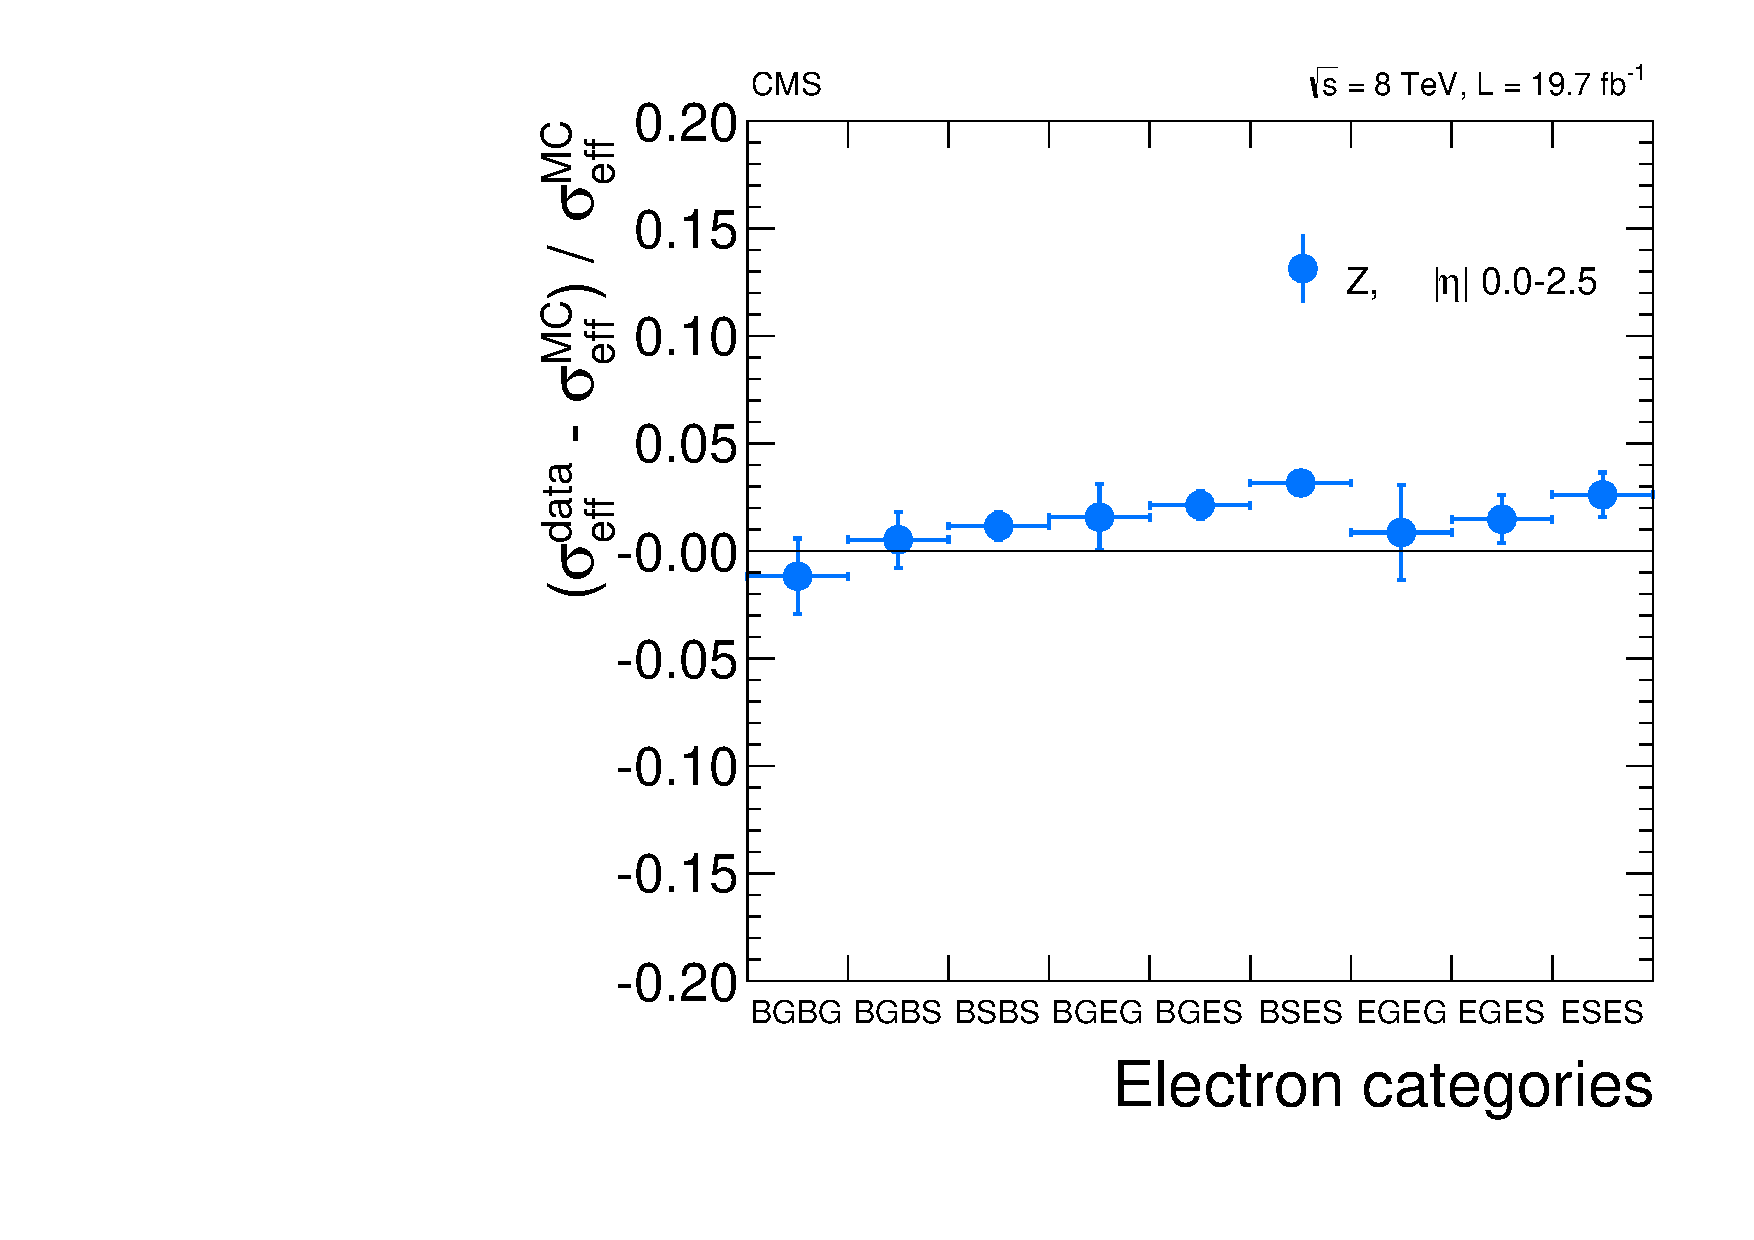
\includegraphics[width=.45\linewidth]{HiggsDiscovery/figures/electron_resolution.pdf}
\caption[Mass Resolution and Bias from Di-electron Decays]{Mass Bias and Resolution between Data and MC Simulation for di-electron decays at $8$ $\rm{TeV}$. For bias measurement (left), $Z\rightarrow e^+e^-$ (blue: solid circles in barrel, open diamonds in $0.8<|\eta|<1.5$, open squares in endcaps) shows little mass bias for higher $p_T$ electrons For lower $p_T$ electrons, $Z\rightarrow e^+e^-$, $J/\Psi\rightarrow e^+e^-$ (solid red circles), and $\Upsilon\rightarrow e^+e^-$ (solid green circles) show a small bias, accounted for as a systematic the signal mass scale. The instrumental mass resolution (right) using $Z\rightarrow e^+e^-$ is less than $4\%$ across the full ECAL range. Electrons are categorized by location and quality of reconstructed electron (B is ECAL Barrel, E for ECAL Endcap. G are the highest quality electron reconstructions, S is for lower quality reconstructions in multiple clusters or with a large amount of bremsstrahlung).}
\label{fig:ElectronMassResolutionAndBias}
\end{center}
\end{figure}

\subsection{Muons}
\label{sec:zz4lMuons}

Muons are reconstructed similar to electrons, except that the matching is done between the inner tracker and the muon system. As with electrons, matching can be ``outside-in" starting with hits in the muon system or ``inside-out" starting with hits in the tracker. By geometric and efficiency constraints, reconstructed muons must have $|\eta^\mu|<2.4$ and $p_T^\mu>5$ $\rm{GeV}$ \cite{}. As muons primarily interact with the tracker and muon system, muons are identified using minimal requirements in the tracker systems to account for consistent trajectories while maintaining small energy deposits in the ECAL \cite{}. The momentum resolution for muons is $1.3-2.0\%$ in the barrel and up to $6\%$ in the endcaps.

Similar to electrons, the muon mass scale and resolution is found using $Z\rightarrow \mu^+\mu^-$, $J/\Psi \rightarrow \mu^+\mu^-$, and $\Upsilon \rightarrow \mu^+\mu^-$ data and MC mass distributions. Across all decays, no bias is seen between data and MC within $0.1\%$, see left plot in Fig.~\ref{fig:MuonMassResolutionandBias}. Muons in the endcaps for the $J/\Psi$ decay have slightly larger offsets, but this is a very unlikely kinematic region for $H\rightarrow ZZ \rightarrow 4l$ events. In the right plot of Fig.~\ref{fig:MuonMassResolutionandBias}, mass resolution is seen to be consistent between data and MC within about $5\%$ for the $Z$ di-muon decay.

\begin{figure}[htbp]
\begin{center}
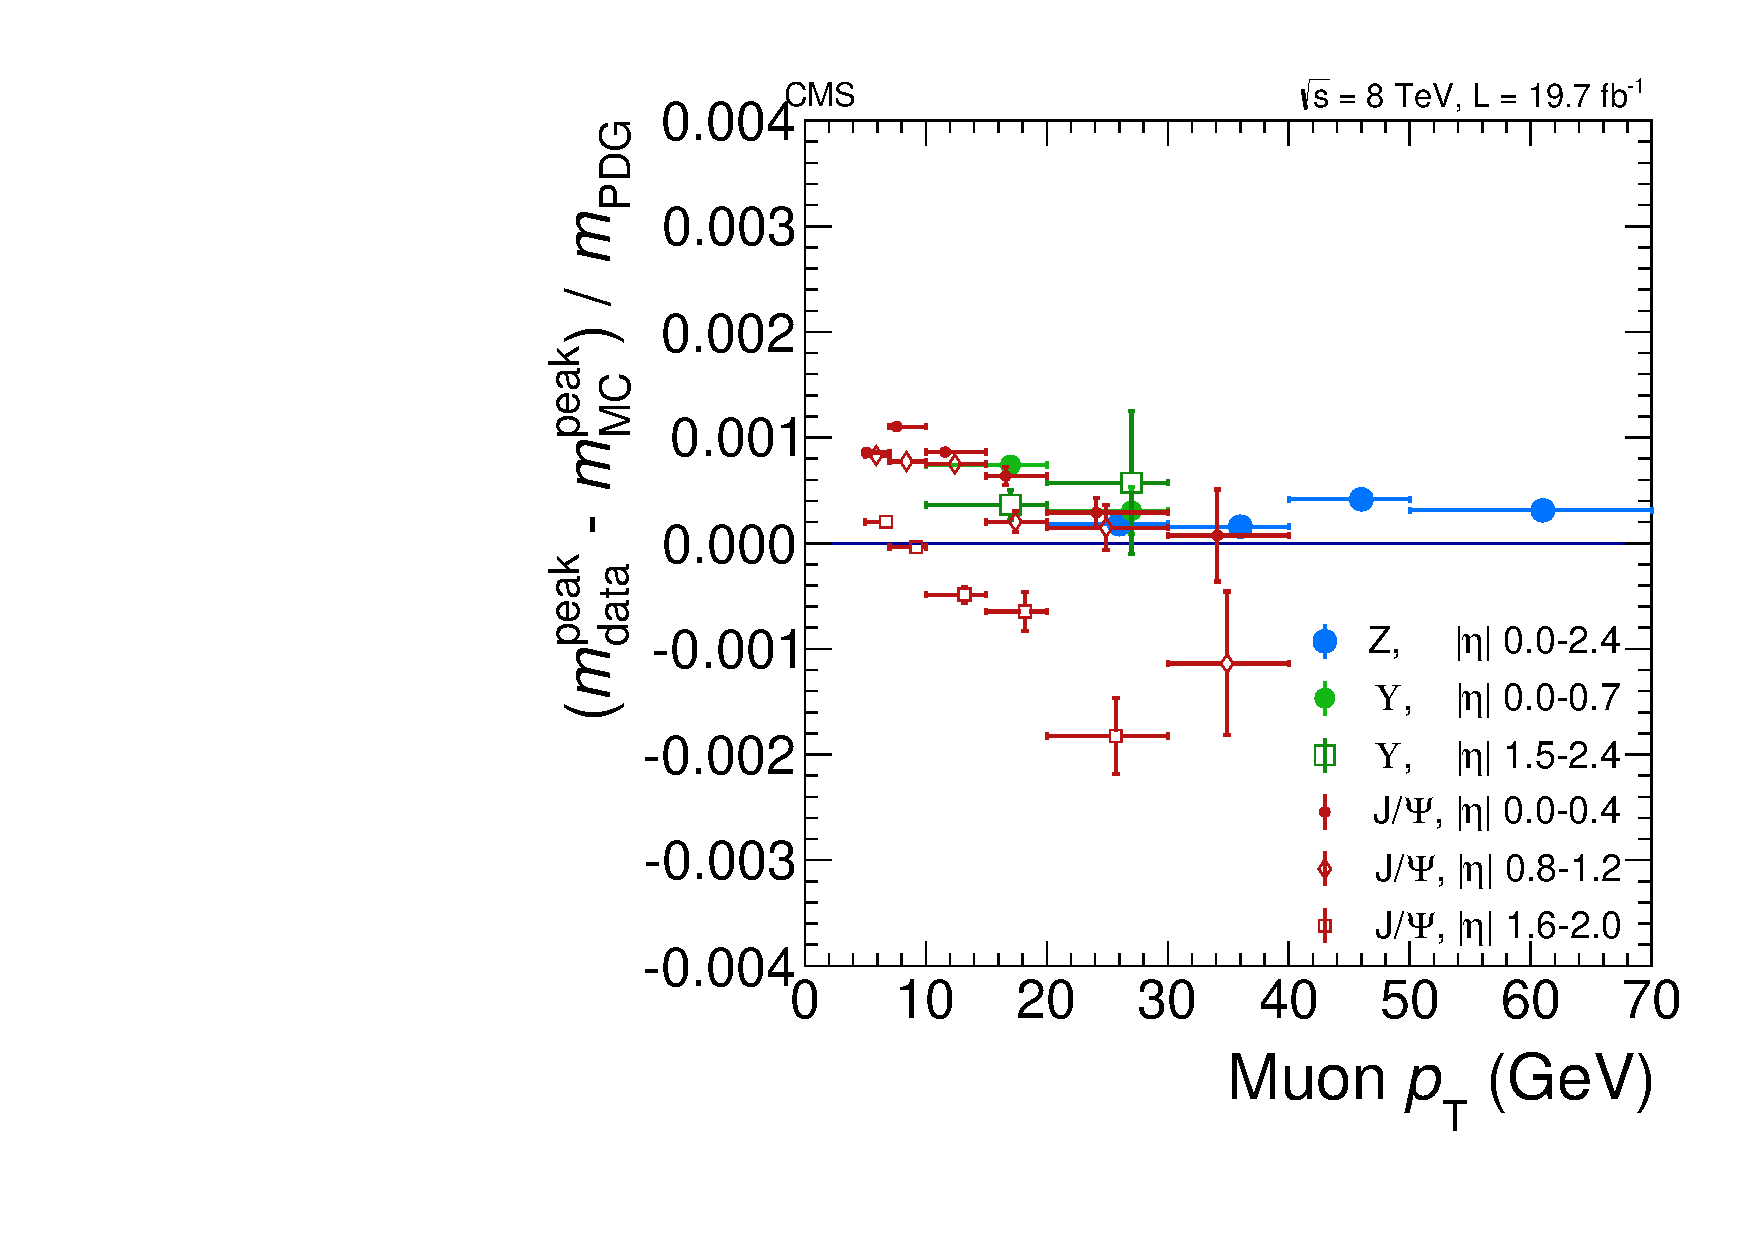
\includegraphics[width=.45\linewidth]{HiggsDiscovery/figures/100_scale_mf.pdf}
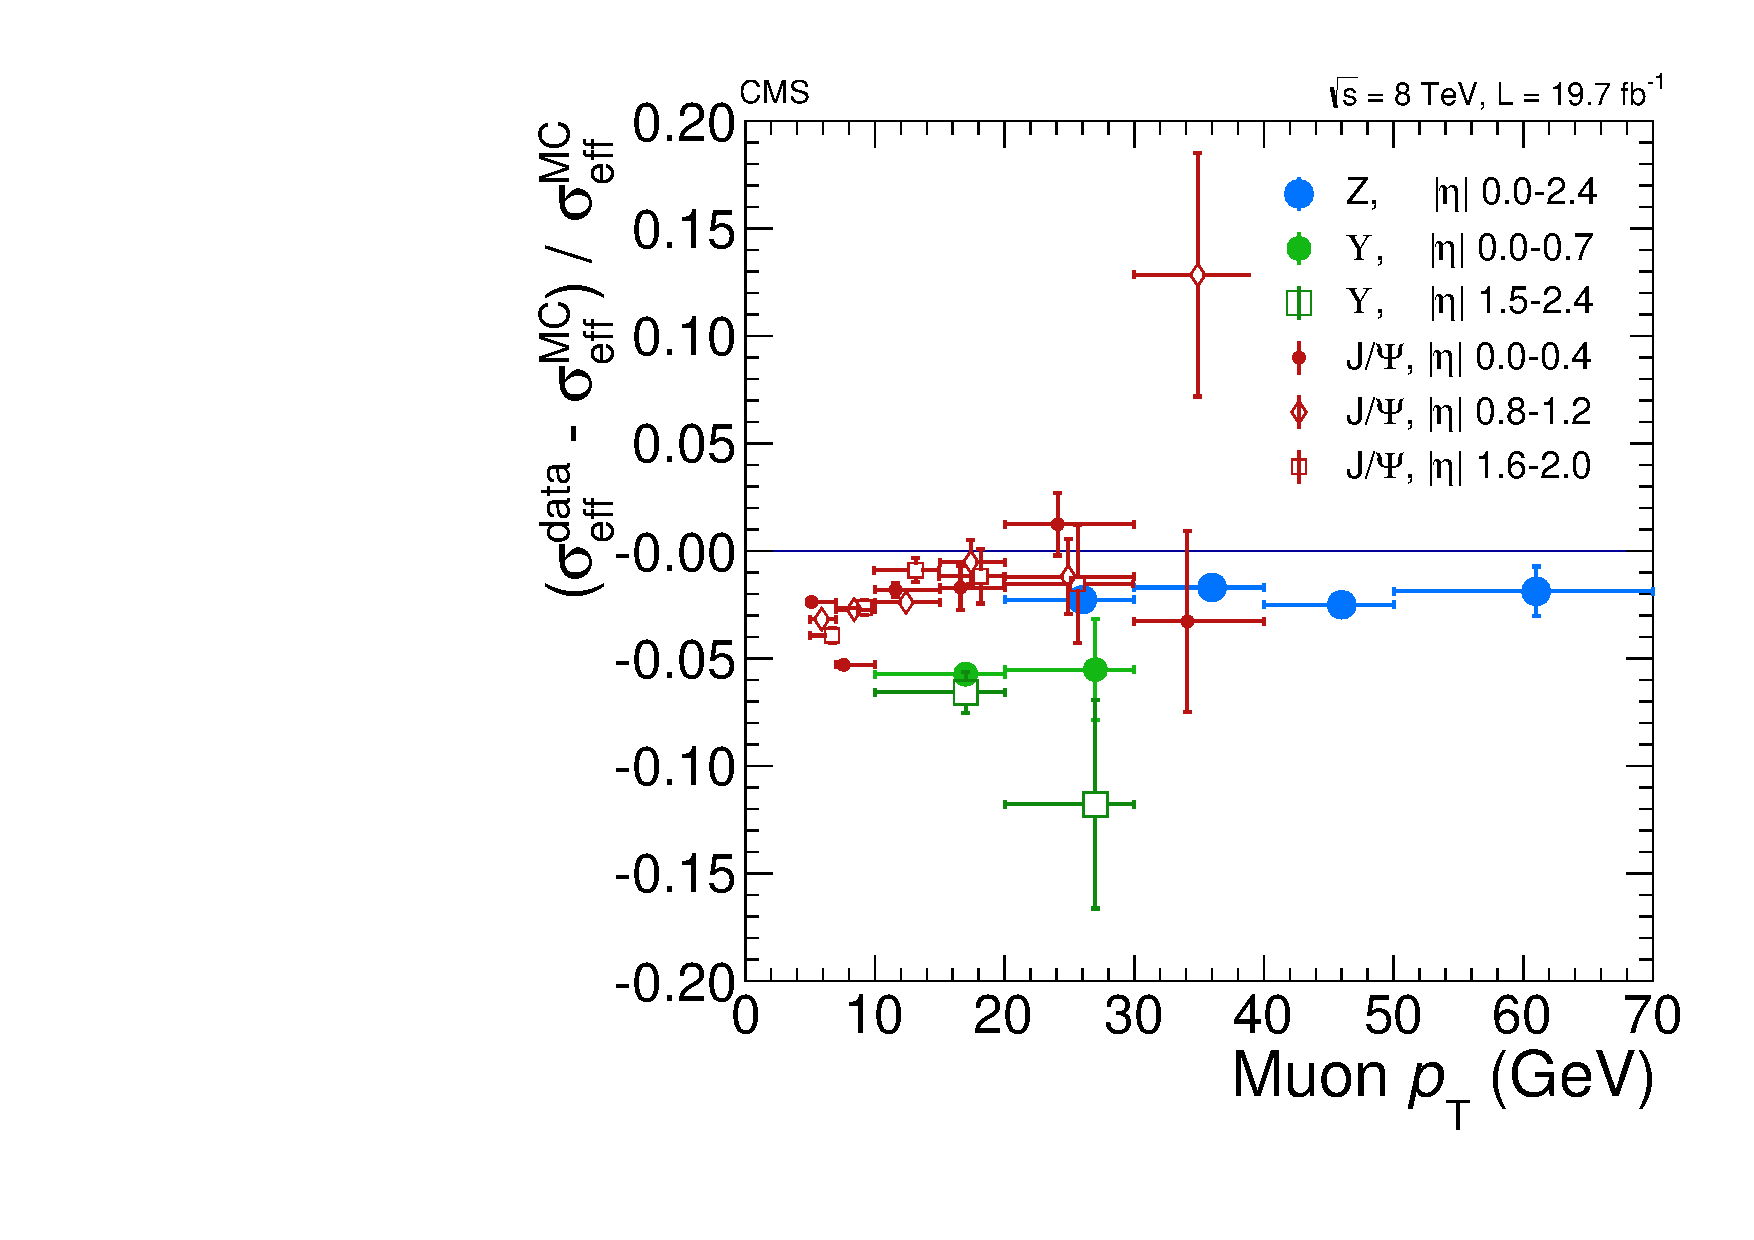
\includegraphics[width=.45\linewidth]{HiggsDiscovery/figures/100_resolution_mf.pdf}
\caption[Mass Resolution and Bias from Di-muon Decays]{Mass Bias (left) and Resolution (right) between Data and MC Simulation for di-muon decays: $Z\rightarrow \mu^+\mu^-$ (blue solid circles), $J/\Psi\rightarrow e^+e^-$ (red: solid circles in barrel, open diamonds in $0.8<|\eta|<1.2$, open squares in endcaps), and $\Upsilon\rightarrow e^+e^-$ (green: solid circles in barrel, open squares in endcaps). Aside from high $p_T$ muonic decays through endcaps, no bias is observed within about $0.1\%$. Mass resolution between $Z$ decays are in agreement within $5\%$.}
\label{fig:MuonMassResolutionandBias}
\end{center}
\end{figure}

\subsection{Lepton Isolation and Photons}
\label{sec:zz4lIsolation}

After reconstruction and identification, leptons should be isolated to confirm that they are a primary decay product. For any given particle flow candidate, the idea of relative isolation is defined by looking at all particles in a cone around the candidate and finding the relative fraction of $p_T$ from particles coming from non-leptonic processes. This is simply affirming that the lepton is the highest momentum object within a given space of the detector. Explicitly, for a cone of size $\Delta R = \sqrt{(\eta^l-\eta^i)^2 + (\phi^l-\phi^i)^2} < 0.4$, where $\eta^l,\phi^l$ are the $\eta$ and $\phi$ of the lepton candidate, the isolation $R_{iso}^l$ is
\begin{equation}
\label{eqn:reliso}
R_{iso}^l \equiv \left( \sum p_T^{\rm{charged}} + \rm{MAX}\left[0, \sum p_T^{neutral} + \sum p_T^{\gamma} - \rho\times A_{\rm{eff}}\right] \right) / p_T^{l}.
\end{equation}

$\sum p_T^{\rm{charged}}$ is the sum of the transverse momentum of any charged hadrons coming from the primary vertex, where the primary vertex is the vertex with the highest $\sum p_T^2$ of constituent tracks. $\sum p_T^{neutral}$ and $\sum p_T^{\gamma}$ are the sums of neutral hadrons and photons that are not radiated by the lepton (see below). When considering particles in this cone, particles very close to the lepton are not considered to avoid double counting.

As stated in Sec.~\ref{sec:ParticleID}, in any event, there are roughly 20-30 different collisions. After identifying the lepton candidates, the subsystems will still have some occupancy from the remaining collisions, called \textit{pileup}. The maximum and the $\rho\times A_{\rm{eff}}$ term in Eqn.~\ref{eqn:reliso} come from mitigating these effects in the neutral components, as the elements of the subsystems will have an average energy density from unassociated processes \cite{}. All isolated leptons in this analysis must have $R_{iso}^l < 0.4$.

After reconstruction, identification, and isolation, the overall efficiencies of electrons and muons are measured using a ``tag and probe" technique \cite{}. Using the large $Z\rightarrow l^+l^-$ dataset, one lepton (either an electron or a muon, depending on what efficiency is being evaluated) that passes all trigger, identification, and selection requirements is used as the ``tag". The $Z\rightarrow l^+l^-$ with background mass shape is then fit using samples where the second lepton, the ``probe", passes or fails the selection cuts. By finding the ratio of efficiencies between data and MC distributions with all associated uncertainties, the simulations can be reweighted in bins of $p_T^{l}$ and $\eta^l$ to account for the overall efficiency. Seen in Fig.~\ref{fig:LeptonEfficiencies}, both electrons and muons have high efficiencies for high $p_T$ leptons ($\gtrsim85\%$ and $\gtrsim97\%$, respectively).

\begin{figure}[htbp]
\begin{center}
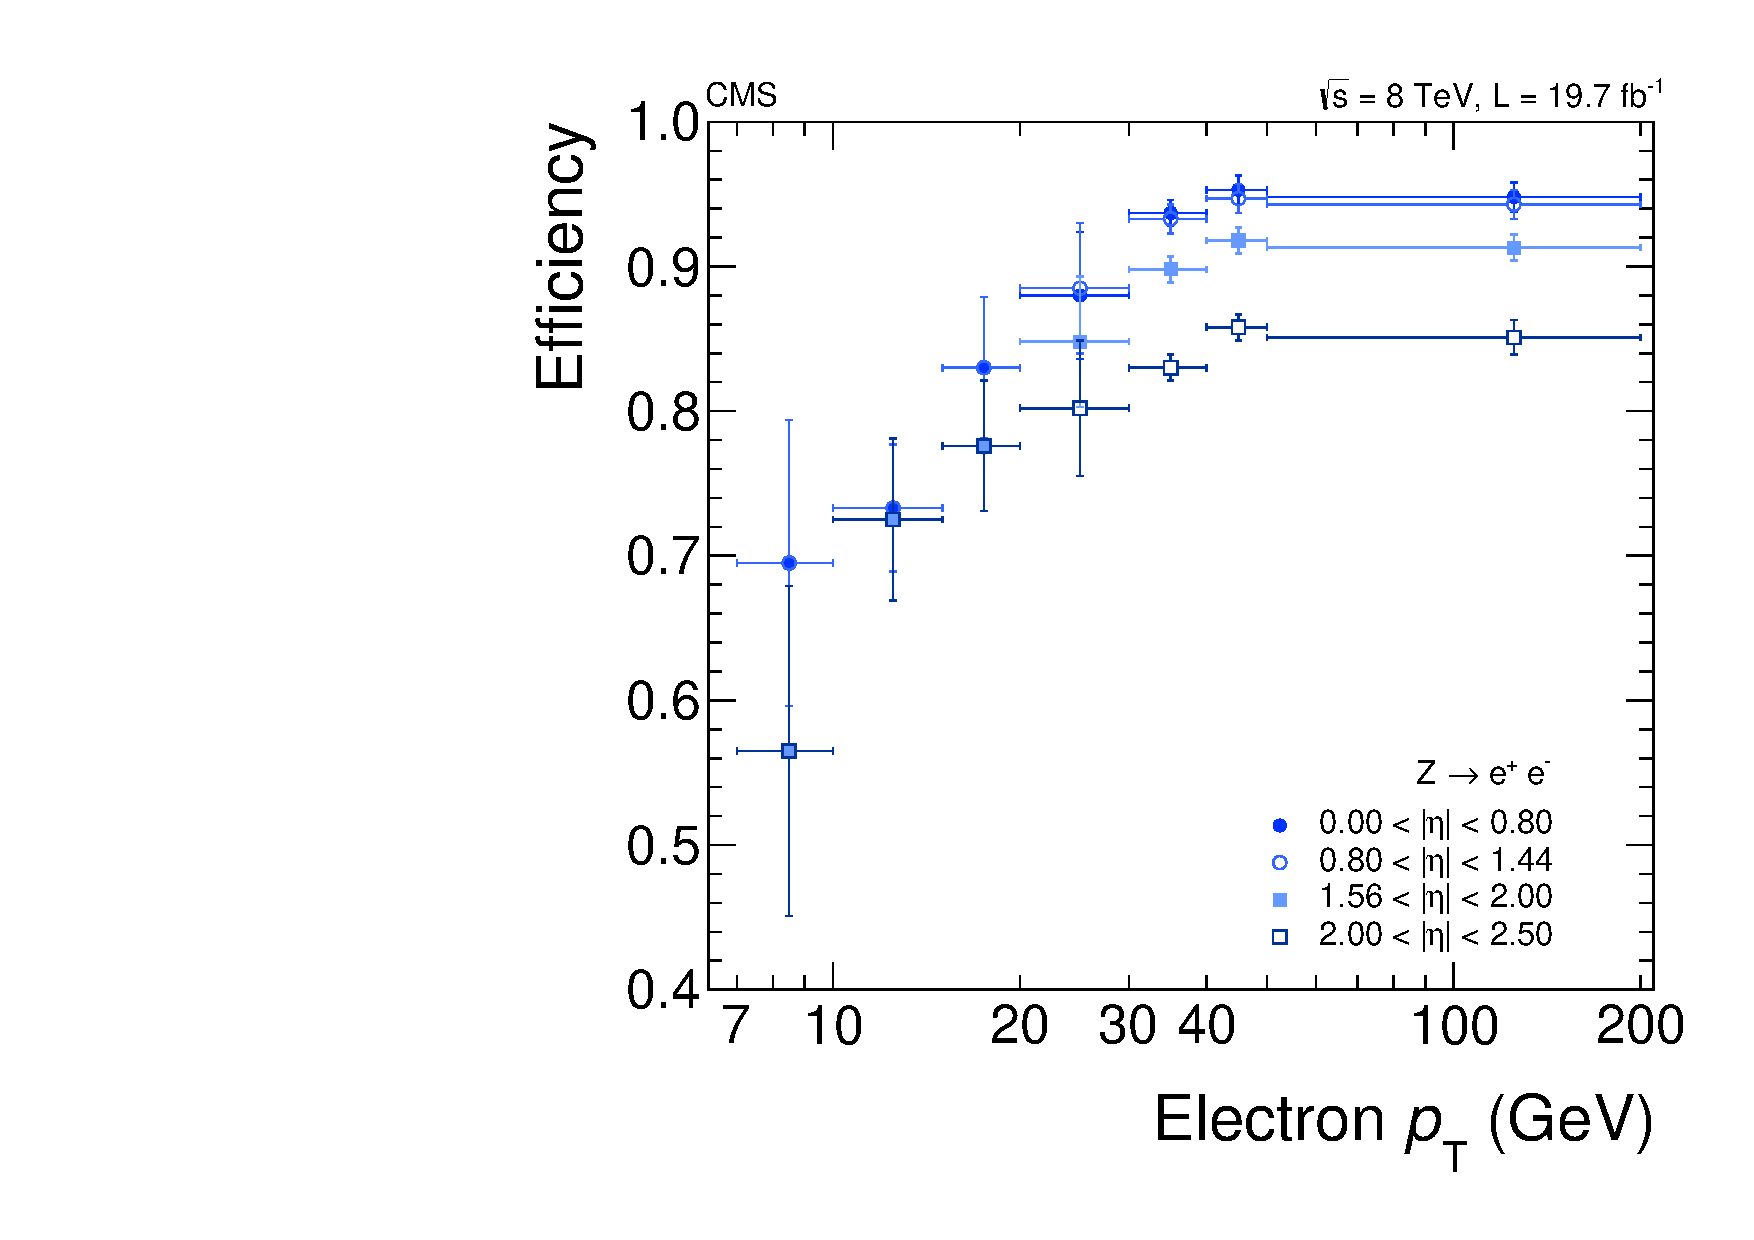
\includegraphics[width=.45\linewidth]{HiggsDiscovery/figures/electron_efficiency.pdf}
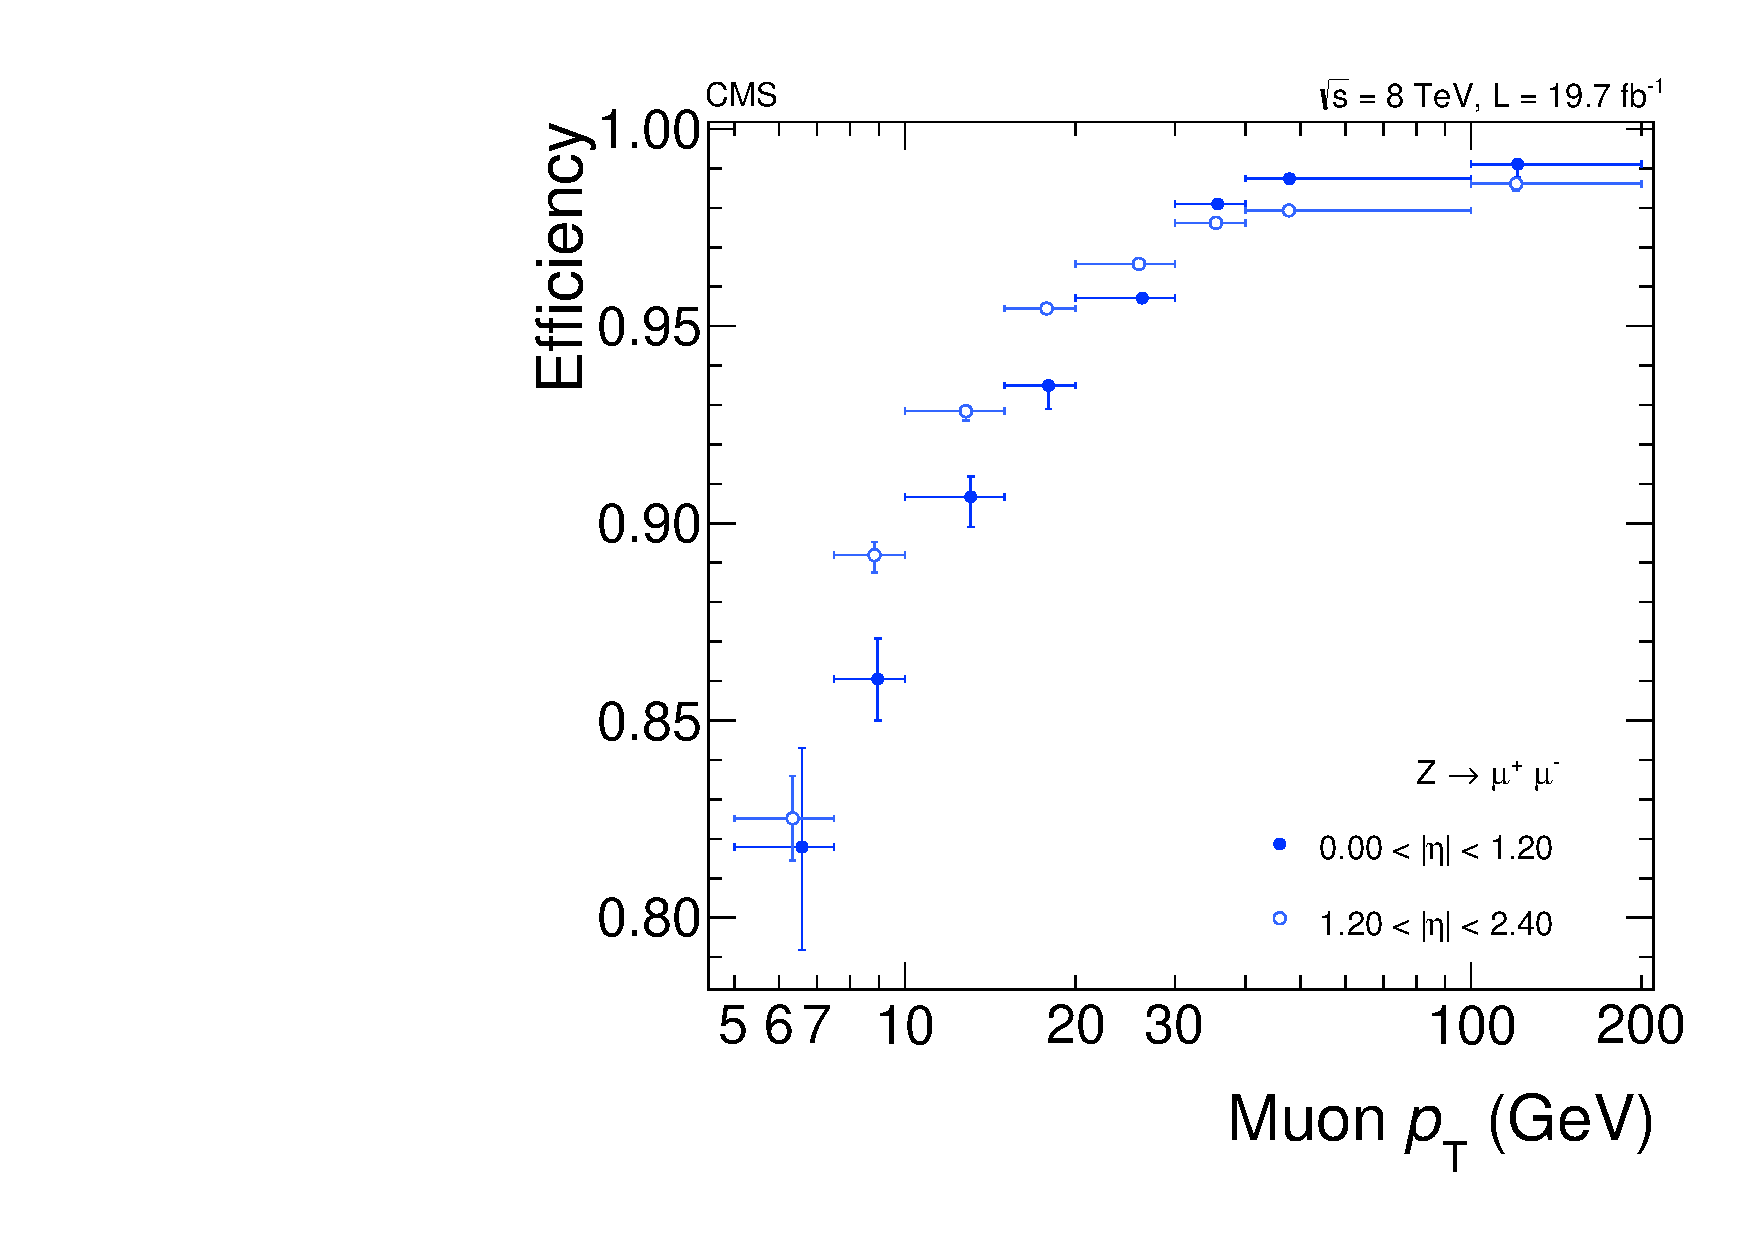
\includegraphics[width=.45\linewidth]{HiggsDiscovery/figures/muon_efficiency.pdf}
\caption[Overall Efficiencies of Electron and Muon Reconstruction and Selection in $4l$ Analysis]{Efficiencies of reconstruction and selection for electrons (left: circles in barrel, squares in endcaps) and muons (right: circles in barrel, squares in endcaps) as functions of $p_T$, found using the tag and probe technique on simulation and data of $Z\rightarrow l^+l^-$. }
\label{fig:LeptonEfficiencies}
\end{center}
\end{figure}


Although photons are not part of this final decay channel, a lepton that decayed from the $Z$ could radiate a photon in its flight through the detector. To properly reconstruct the full kinematics, these \textit{final state radiation} (FSR) photons must be accounted for. FSR photons, having radiated from a lepton, must be close to a lepton candidate and have sufficient momentum to be considered a significant correction. Photons are accepted as FSR if: i) they fall in similar geometric boundaries as leptons ($|\eta^\gamma|<2.4$) and ii) have $p_T>2$ $\rm{GeV}$ if within $\Delta R < 0.07$ of a lepton OR $p_T>4$ $\rm{GeV}$ if found isolated within $0.07 < \Delta R < 0.5$ of a lepton candidate. An isolated photon is defined, similar to Eqn.~\ref{eqn:reliso}, as $R_{iso}^{\gamma} = (\sum p_T^{charged} + \sum p_T^{neutral} + \sum p_T^{photons})/p_T^\gamma < 1$ where the sums the same except over a cone of $\Delta R < 0.3$.

\subsection{Jets}
\label{sec:zz4lJets}

Once any lepton and FSR photon candidates are determined, jet candidates are identified. Jets are found using the HCAL and tracker, where they are reconstructed using the anti-$k_T$ clustering algorithm\footnote{As stated in Sec.~\ref{sec:HadrCalo}, jets come from the hadronization and fragmentation of particles that interact via the strong force. Different clustering algorithms have been developed to group tracks and calorimeter hits inside cones into jet objects.} \cite{} with distance parameter $R=0.5$, implemented using the {\tt FASTJET} package \cite{}. Jet energy corrections as functions of $E_T$ and $\eta$ are applied to calibrate the energy of a detected jet with the expected true energy \cite{}. To separate jet candidates from pileup, a discriminant is built \cite{} via a multivariate analysis using BDTs where the number vertices, jet shapes, relative multiplicity of charged and neutral components, and fraction of low-$p_T$ components are used for training. The tracks of any selected jets must be compatible with the primary vertex, as true for lepton candidates. Finally, jets must also have sufficiently high momentum ($p_T>30$ $\rm{GeV}$) and separated from any leptons or FSR photons ($\Delta R = \sqrt{(\eta^{l/\gamma}-\eta^{jet})^2 + (\phi^{l/\gamma}-\phi^{jet})^2} > 0.5$).

\section{MC and Datasets}
\label{sec:ZZ4lMCandData}

With objects defined, MC samples are generated for both background and signal processes. These samples can establish optimal event selections and quantify uncertainties. The full list of MC Samples can be found in Table~\ref{tbl:MCSamples}. 

\begin{table}[htbp]
  \begin{center}
  \vspace*{0.3cm}
  \renewcommand{\arraystretch}{0.5}
    \begin{tabular}{lllll} 
\hline %---------------------------------------------------------------------------------------------------------------------------------------------------------------------------- 
\small      \bf{Process} 		& \small \bf{MC}			& \multicolumn{2}{c}{\small\boldmath{$\sigma_{(N)NLO} $}} & \small\bf{ Comments and sample name}  \\
     					& \small \bf{generator}			& \small $7$ $\rm{TeV}$ 	& \small $8$ $\rm{TeV}$        			  &		                          \\ 
\hline \hline %=====================================================================================================================================================================
%
         \multicolumn{5}{l}{\small  \bf{Higgs boson}   $H \rightarrow ZZ \rightarrow 4\ell$} \\
%     	      
\small         ${gg} \rightarrow H$ & \small{\tt POWHEG}  & \small [1-20] fb 	& \small [1.2-25] fb        & \small{\small $\mathrm{m_{H}=110}$-$1000$ $\rm{GeV}$}  \\ 
\small         $VV \rightarrow H$   & \small{\tt POWHEG}  & \small [0.2-2] fb 	& \small [0.3-25] fb        & \small{\small $\mathrm{m_{H}=110}$-$1000$ $\rm{GeV}$}  \\ 
\small         $V^{*} \rightarrow VH$   & \small{\tt PYTHIA}  & \small [] fb 	& \small [] fb        & \small{\small $\mathrm{m_{H}=110}$-$200$ $\rm{GeV}$}  \\ 
\small         $t\bar{t}H$   & \small{\tt PYTHIA}  & \small [] fb 	& \small [] fb        & \small{\small $\mathrm{m_{H}=110}$-$200$ $\rm{GeV}$}  \\ 
\hline %---------------------------------------------------------------------------------------------------------------------------------------------------------------------------- 
         \multicolumn{5}{l}{{\small   \bf ZZ continuum } } \\
\small    $ q\bar{q} \rightarrow ZZ \rightarrow 4e(4\mu,4\tau) $           
                                    	  & \small{\tt POWHEG}	& \small 66.09 fb	& \small 76.91 fb	    & \small{\small ZZTo4e(4mu,4tau)}  \\ 
\small	 $ q\bar{q} \rightarrow ZZ \rightarrow 2e2\mu  $           
                                    	  & \small{\tt POWHEG}	& \small 152 fb	& \small 176.7 fb	    & \small{\small ZZTo2e2mu}  \\ 
\small	 $ q\bar{q} \rightarrow ZZ \rightarrow 2e(2\mu)2\tau  $           
                                    	  & \small{\tt POWHEG}	& \small 152 fb	& \small 176.7 fb	    & \small{\small ZZTo2e(2mu)2tau}  \\ 
\small      ${gg} \rightarrow ZZ \rightarrow 2\ell 2\ell'$              
      					  & \small{\tt gg2ZZ}  	& \small 3.48 fb 	& \small 12.03  fb	    & \small{\small GluGluToZZTo2L2L} \\ 
\small      ${gg} \rightarrow ZZ \rightarrow 4\ell$                
         				  & \small{\tt gg2ZZ}  	& \small 1.74 fb 	& \small 4.8 fb	    & \small{\small GluGluToZZTo4L} \\  
					 \hline
         \multicolumn{5}{l}{{\small  \bf Other di-bosons} } \\
\small	 $WW\rightarrow 2\ell2\nu $   & \small{\tt Madgraph}  & \small 4.88 pb   	& \small 5.995 pb 	    & \small{\small WWJetsTo2L2Nu} \\ 
\small	 $WZ\rightarrow 3\ell\nu $    & \small{\tt Madgraph}  & \small 0.868 pb 	& \small 1.057 pb  	    & \small{\small WZJetsTo3LNu} \\  
\hline %---------------------------------------------------------------------------------------------------------------------------------------------------------------------------- 
         \multicolumn{5}{l}{\small   \boldmath{$t\bar{t}$ and single $t$ }} \\
\small   $t\bar{t} \rightarrow \ell^+\ell^- \nu\bar{\nu} b\bar{b}$ & \small{\tt POWHEG}		& \small 17.32 pb    & \small 23.64 pb 	& \small{\small TTTo2L2Nu2B} \\       
\small   $t$ ($s$-channel)   		& \small{\tt POWHEG} 		& \small 3.19 pb 	& \small 3.89 pb 			& \small{\small T\_TuneXX\_s-channel} \\        
\small   $\bar{t}$ ($s$-channel)   	& \small{\tt POWHEG} 		& \small 1.44 pb 	& \small 1.76 pb 			& \small{\small Tbar\_TuneXX\_s-channel} \\       
\small   $t$ ($t$-channel)   		& \small{\tt POWHEG} 		& \small 41.92 pb 	& \small 55.53 pb				& \small{\small T\_TuneXX\_t-channel} \\        
\small   $\bar{t}$ ($t$-channel)   	& \small{\tt POWHEG} 		& \small 22.65 pb 	& \small 30.00 pb				& \small{\small Tbar\_TuneXX\_t-channel} \\
\small   $t$ ($tW$-channel)   		& \small{\tt POWHEG} 		& \small 7.87 pb 	& \small 11.77 pb				& \small{\small T\_TuneXX\_tW-channel-DR} \\        
\small   $\bar{t}$ ($tW$-channel)   	& \small{\tt POWHEG} 		& \small 7.87 pb 	& \small 11.77 pb				& \small{\small Tbar\_TuneXX\_tW-channel-DR} \\ 
\hline %---------------------------------------------------------------------------------------------------------------------------------------------------------------------------- 
          \multicolumn{5}{l}{\bf{Z/W + jets ($q=d,u,s,c,b$)}} \\     
\small   $W$ + jets     			& \small{\tt MadGraph}		& \small 31314 pb         & \small 36257.2 pb			& \small{\small WJetsToLNu} \\
\small   $Z$ + jets, m$_{\ell\ell}>50$     		& \small{\tt MadGraph}		& \small 3048 pb           & \small 3503.7 pb			& \small{\small DYJetsToLL*M-50} \\ 
\small   $Z$ + jets, $10<m_{\ell\ell}<50$     	& \small{\tt MadGraph}		& \small 12782.63 pb    & \small 915   pb			& \small{\small DYJetsToLL*M-10To50} \\ 
\hline %---------------------------------------------------------------------------------------------------------------------------------------------------------------------------- 
%          \multicolumn{5}{l}{ \small  \bf{QCD inclusive multi-jets}, {\small binned  $\Hat{p}_T^{\rm min}$}} \\    
%{\small $b,c \rightarrow e + X$}   	& \small{\tt PYTHIA}		& \small		& \small				& \small {\small QCD\_Pt-XXtoYY\_BCtoE }   \\
%\small  EM-enriched   			& \small{\tt PYTHIA}		& \small		& \small				&\small {\small QCD\_Pt-XXtoYY\_EMEnriched } \\
%\small   MU-enriched   			& \small{\tt PYTHIA}		& \small 		& \small				& \small {\small QCD\_Pt-XXtoYY\_MuPt5Enriched }  \\ 
%\hline%---------------------------------------------------------------------------------------------------------------------------------------------------------------------------- 
   \end{tabular}
\caption[MC Samples for $H\rightarrow ZZ\rightarrow 4l$]{Full List of MC Samples generated for $H\rightarrow ZZ\rightarrow 4l$, with their respective processes, generators, cross-sections for $\rm{7}$ $\&$ $\rm{8}$ $\rm{TeV}$ at the generated order, and sample names.}
  \label{tbl:MCSamples}
  \end{center}
\end{table}

For signal samples, gluon-gluon fusion and vector boson fusion are generated at next-to-leading order using {\tt POWHEG} \cite{} up to masses of $m_H = 1000$ $\rm{GeV}$. Higgs produced via Higgsstrahlung ($WH$ or $ZH$) or associated production ($t\bar{t}H$) are generated using {\tt PYTHIA} \cite{} at LO. Since their expected cross sections are smaller for higher masses (see Fig.~\ref{fig:HXSWGProduction}), they are only generated up to $m_H=200$ $\rm{GeV}$.

There are two additional complications for the Higgs signal samples. First, for lower masses, the Higgs can be modeled to have approximately zero-width, that is the mass distribution in $m_{4l}$ will be a very narrow resonance. For a higher mass Higgs, the number of energetically viable decay modes increases, so this approximation breaks down\footnote{This approximation also isn't entirely valid for a lower mass Higgs, as we shall see in Sec.~\ref{sec:Width}.} around $m_H \approx 400$ $\rm{GeV}$, as seen in Fig.~\ref{fig:HiggsWidth}. To account for this, the mass shape uses the complex-pole scheme \cite{,,}. Second, gluon-fusion Higgs production with $4l$ decay has identical initial and final states as the $gg\rightarrow 4l$ background, so they will interfere (see Sec.~\ref{sec:FeynDiagrams}, diagrams with identical initial and final states can interfere). Below $2\times m_Z$, this effect is negligible, because the $gg\rightarrow 4l$ background is small, but it must be accounted for in high mass Higgs samples. Additionally, signal events are reweighted to the total $pp\rightarrow H$ cross section, including NNLO and next-to-next-to-leading log\footnote{Corrections from additional Feynman diagrams can also have logarithmic dependencies.} corrections for gluon fusion \cite{} and NNLO contributions for VBF \cite{}.

\begin{figure}[htbp]
\begin{center}
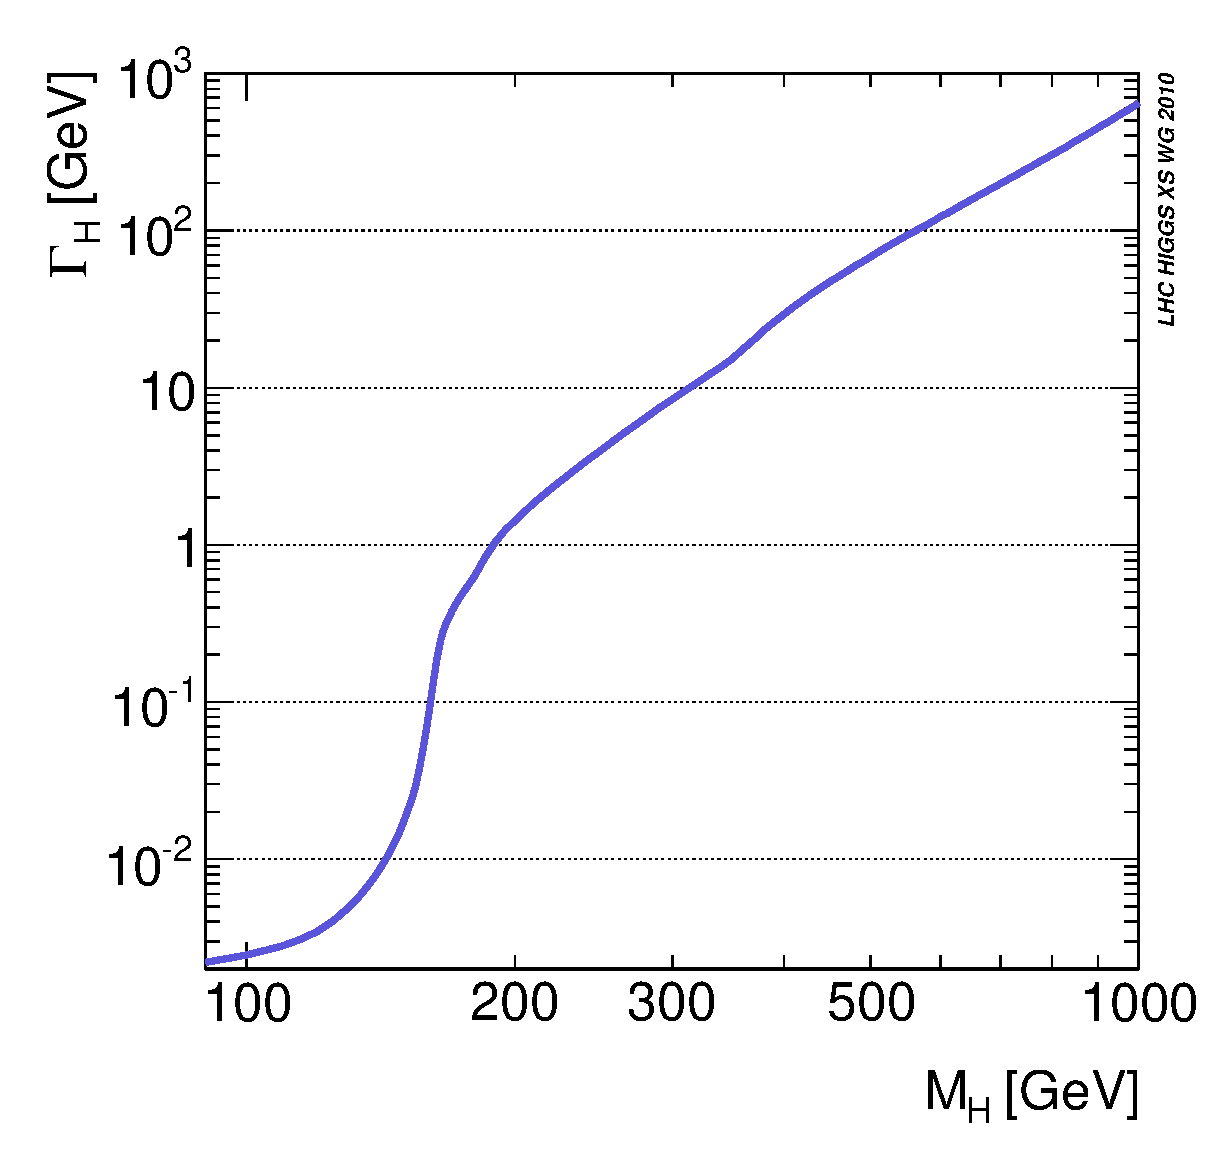
\includegraphics[width=.5\linewidth]{HiggsDiscovery/figures/HiggsWidth}
\caption[Higgs Width as a Function of $m_H$]{Higgs Width as a Function of $m_H$. The width of the mass shape for the Higgs depends on the available decay modes at a given mass. For $m_H > 2\times m_Z$, both bosonic decays will be on-shell (see Sec~\ref{sec:HiggsDecay}), drastically increasing the width compared to low $m_H$.}
\label{fig:HiggsWidth}
\end{center}
\end{figure}

We can categorize background into \textit{reducible} and \textit{irreducible} backgrounds. Reducible backgrounds come from large cross section SM processes where two prompt isolated leptons are generated and the remaining two, coming from secondary decays unrelated to the desired $ZZ\rightarrow 4l$ vertex, are misidentified leptons. $Z$ + jets, for example, can have two isolated leptons from the $Z$ but occasionally two $b$-jets will be produced which can be misidentified as leptons. Similarly, $t\bar{t}$ commonly decays to a state with $l^+l^-b\bar{b}$. $W/Z$ + jets samples are produced using {\tt MADGRAPH} \cite{}, while any $t$ samples are made using {\tt POWHEG}. As the name implies, a smart selection (see Sec.~\ref{sec:ZZ4lSelection}) can reduce this background substantially.

Irreducible backgrounds are SM processes that have identical decay channels as the intended Higgs signal events, arising from the $ZZ$ continuum background. The primary irreducible background is $q\bar{q}\rightarrow 4l$, as seen in the left diagram of Fig.~\ref{fig:IrreducibleBackFeyn}, generated at NLO using {\tt POWHEG}. $gg \rightarrow 4l$, in the right diagram of Fig.~\ref{fig:IrreducibleBackFeyn}, is the subdominant irreducible background as it requires one loop to be produced. It was generated using {\tt GG2ZZ} \cite{}.

\begin{figure}
\begin{center}
\unitlength=1mm
\subfloat{
\begin{fmffile}{HiggsDiscovery/figures/qqZZBackground}
\begin{fmfgraph*}(60,40)
  \fmfstraight
  \fmfleft{i1,i2}
  \fmfright{sp1,sp2,sp3,sp4}
  \fmf{fermion,label=$q$,label.side=left,tension=2}{i1,v1}
  \fmf{fermion}{v1,v2}
  \fmf{fermion,label=$\bar{q}$,label.side=left,tension=2}{v2,i2}
  \fmf{photon,label=$Z/\gamma$}{v1,vo1}
  \fmf{photon,label=$Z/\gamma$}{v2,vo2}
  \fmf{phantom}{vo1,vo2}
  \fmf{phantom,tension=2}{vo1,sp1}
  \fmf{phantom,tension=2}{vo2,sp4}
  \fmffreeze
  \fmf{fermion,label=$l^{+}$,label.side=left}{sp1,vo1}
  \fmf{fermion,label=$l^{-}$}{vo1,sp2}
  \fmf{fermion,label=$l^{+}$,label.side=left}{sp3,vo2}
  \fmf{fermion,label=$l^{-}$}{vo2,sp4}
\end{fmfgraph*}
\end{fmffile}
}
\subfloat{
\begin{fmffile}{HiggsDiscovery/figures/ggZZBackground}
\begin{fmfgraph*}(60,40)
  \fmfstraight
  \fmfleft{i1,i2} \fmfright{o1,o2,o3,o4}
  \fmf{gluon,label=$g$,tension=2}{i1,v1} \fmf{gluon,label=$g$,tension=2}{i2,v2}
  \fmf{fermion}{v1,v2}
  \fmf{fermion}{v3,v4}
  \fmf{fermion,label=$q$,tension=2}{v2,v3}
  \fmf{fermion,label=$\bar{q}$,tension=2}{v4,v1} 
  \fmf{phantom,tension=2}{v4,o1}
  \fmf{phantom,tension=2}{v3,o4}
  \fmffreeze
  \fmf{photon,label=$Z/\gamma$,l.s=right}{v4,vo1}
  \fmf{photon,label=$Z/\gamma$}{v3,vo2}
  \fmf{fermion,label=$l^{+}$,label.side=left,l.d=2}{o1,vo1}
  \fmf{fermion,label=$l^{-}$,label.side=left,l.d=2}{vo1,o2}
  \fmf{fermion,label=$l^{+}$,l.s=left,l.d=2}{o3,vo2}
  \fmf{fermion,label=$l^{-}$,l.s=left,l.d=2}{vo2,o4}
\end{fmfgraph*}
\end{fmffile}
}
\end{center}
\caption[Irreducible $ZZ$ Backgrounds in the $4l$ Channel]{Feynman Diagrams for the Irreducible Backgrounds in the $4l$ channel. $q\bar{q}\rightarrow 4l$ (left) is dominant, while $gg\rightarrow 4l$ (right) requires a loop and is subdominant.}
\label{fig:IrreducibleBackFeyn}
\end{figure}

All generated background and signal samples interface with {\tt PYTHIA} to produce hadronization and low-$p_T$ radiation effects. After this stage, every sample was processed through software built on {\tt GEANT4} \cite{} which simulates further decays and geometric acceptances in CMS, then reconstructs objects using the same algorithms applied on data, accounting for any pileup effects. For any LO generators, the PDF used for generation is {\tt CTEQ6L} \cite{}. For NLO generators, {\tt CT10} \cite{} is used. 

The datasets used are from the 2011 $7$ $\rm{TeV}$ and 2012 $8$ $\rm{TeV}$ runs, with luminosities of $5.1 fb^{-1}$ and $19.7 fb^{-1}$, respectively. Triggers that require at least a pair of leptons are used. For any double lepton trigger (di-electron, di-muon, or muon and electron), at least one lepton must have $p_T>17$ $\rm{GeV}$ and the other must have $p_T>8$ $\rm{GeV}$. A triple electron trigger is also used where the \textit{leading} (highest $p_T$) electron must have $p_T>15$ $\rm{GeV}$, the \textit{subleading} (second highest $p_T$) electron must have $p_T>8$ $\rm{GeV}$, and the third electron must have $p_T>5$ $\rm{GeV}$.

\section{Event Selection}
\label{sec:ZZ4lSelection}

After finding four prompt isolated leptons, most of the reducible background is already suppressed, but because the cross sections of the reducible processes are so large they should be minimized. For the $ZZ \rightarrow 4l$ decay, the $Z$ decays are prompt so all four leptons should appear to come from one common vertex. Upon reconstruction of a primary vertex, the three dimensional distance of closest approach for a trajectory is called the \textit{impact parameter}, which has an associated uncertainty of $\sigma_{\rm{IP}}$. To confirm a common vertex, a cut of $|\rm{SIP_{3D}}=\frac{\rm{IP}}{\sigma_{\rm{IP}}}|<4$ is applied. Leptons that fail either the $|\rm{SIP_{3D}}|<4$ cut or the earlier $R_{iso}^l<0.4$ cut are considered \textit{loose} leptons\footnote{Loose leptons also have relaxed constraints on electron or muon identification but must be separated by at least $\Delta R>0.02$.}, to be used in the estimate of the reducible backgrounds (see Sec.~\ref{sec:ZZ4lMassShape}). On top of the $p_T$ cuts from any triggers, the leading lepton must have $p_T > 20$  $\rm{GeV}$ and the subleading lepton must have $p_T > 10$ $\rm{GeV}$ to improve efficiency.

Next, we construct $Z$ candidates out of the available leptons. The pair of opposite charge and matching flavor leptons (e.g. $e^+e^-$ and $\mu^+\mu^-$) with an invariant mass closest to $m_Z$ is considered $Z_1$, such that $40< m_{Z1} < 120$ $\rm{GeV}$. This cut eliminates nearly all backgrounds that do not contain a leptonic $Z$ decay (e.g. $t\bar{t}$, $W$ + jets) as it is unlikely to get an invariant mass near $m_Z$ otherwise.

Out of the remaining isolated leptons, another pair of opposite charge matching flavor leptons form $Z_2$. For a lower mass Higgs, it's expected that one $Z$ would be on-shell while the other would be off-shell. To optimize for these low mass signals\footnote{For Higgs events with $m_H > 2m_Z$, both of the $Z$ candidates should be on-shell which is accounted for by restricting $m_Z1,2 < 120$ $\rm{GeV}$.}, $m_{Z2}$ has a looser mass cut such that $12 < m_{Z2} < 120$ $\rm{GeV}$. If there are multiple $Z_2$ candidates, as can be the case for five or more isolated leptons, the $Z_2$ candidate with the highest scalar sum of $p_T$ is chosen as these leptons should have the highest reconstruction efficiency. For both $Z_1$ and $Z_2$, if there are any FSR leptons associated with one of the constituent leptons, only those that bring $m_{Z1,2}$ closer to $m_Z$ are kept so long as $m_{ll\gamma}<100$ $\rm{GeV}$.

The requirement for $Z_2$ eliminates most of the remaining reducible $Z+X$ background for the same reason that the $Z_1$ cut eliminates other leptonic background. However, to avoid possible contamination from low-mass hadronic decays faking leptons, any opposite charge pairing of the selected four must have a sufficient invariant mass such that $m_{ll'} > 4$ $\rm{GeV}$. 

Finally, given the earlier direct exclusions from LEP (see Sec.~\ref{sec:findinghiggs}), a cut of $m_{4l} >100$ $\rm{GeV}$ is applied. After object definitions and selection cuts, the final efficiencies of signal detection as a function of the Higgs mass are seen in Fig.~\ref{fig:HiggsEffic}. In general, the $4\mu$ mode has the highest efficiency due to the quality of reconstruction compared to electrons. The relative increase in efficiency past $m_H \approx 200$ $\rm{GeV}$ comes from both $Z$ candidates being on-shell. Polynomial parameterizations are built for the MC signal mass points such that a full range of masses can be examined, as used in Sec.~\ref{sec:ZZ4lAnalysis}.

\begin{figure}[htbp]
\begin{center}
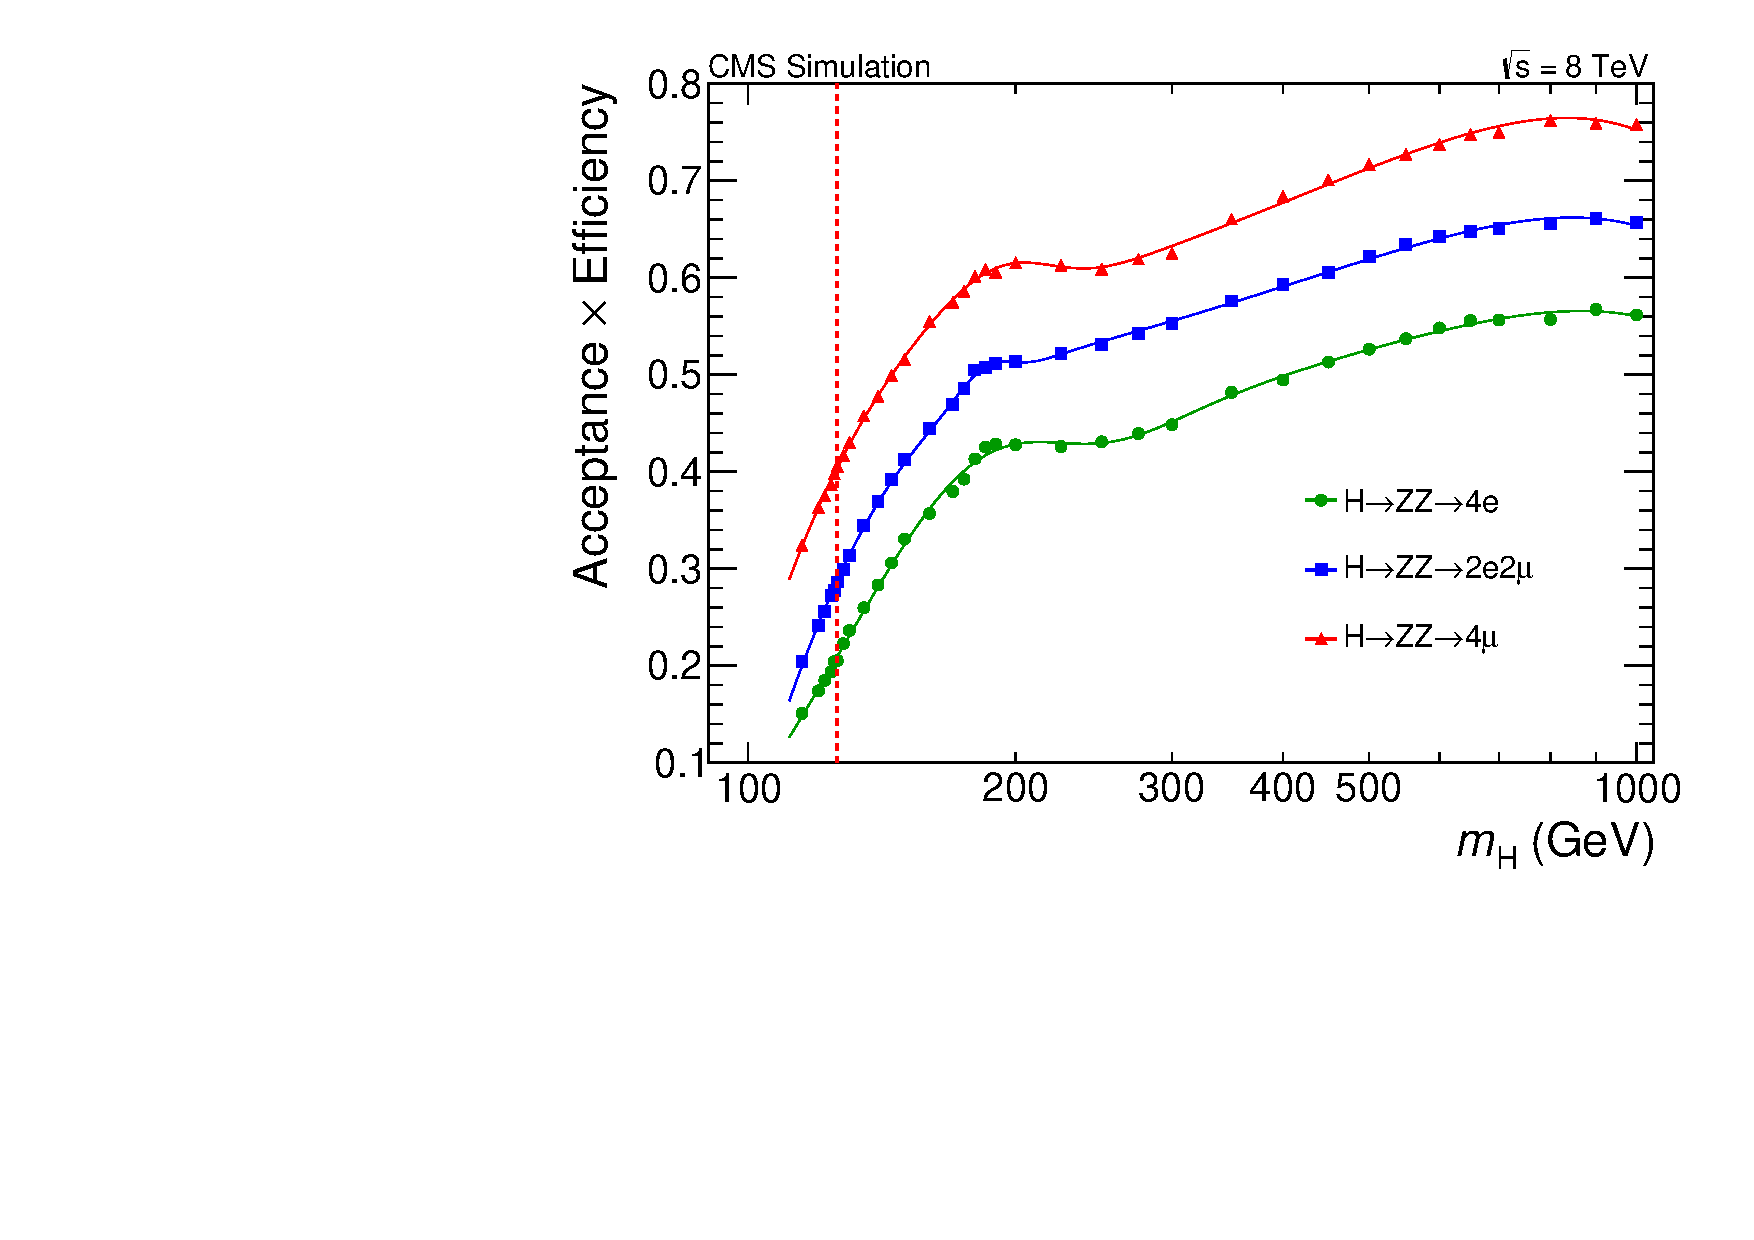
\includegraphics[width=.6\linewidth]{HiggsDiscovery/figures/Efficiency_ggH_8TeV.pdf}
\caption[Signal Efficiency of Gluon Fusion as a Function of $m_H$]{Signal detection efficiencies of ggF as functions of $m_H$, fit with polynomial curves estimated from MC simulation. $4\mu$ (red triangles) has the highest relative efficiency as muon have better selection efficiency, while $4e$ (green circles) has the lowest from electrons having worse efficiency. $2e2\mu$ (blue squares) is between the two. Efficiencies are produced for all production methods with similar results.}
\label{fig:HiggsEffic}
\end{center}
\end{figure}

\section{Likelihood Analysis}
\label{sec:ZZ4lAnalysis}

All observed events are split into tweleve different sub-categories: two for beam energy ($7$ or $8$ $\rm{TeV}$), three for final states ($4e$, $4\mu$, or $2e2\mu$), and two for jet categorization ($\geq2$ jets or $<2$ jets). The likelihood analysis is built on a three-dimensional model of observables: $m_{4l}$, $\mathcal{D}_{\rm{bkg}}^{\rm{kin}}$ and $p_T$ or $D_{jet}$, where the final observable is determined by the jet category. Instead of applying a full three-dimensional fit, the model is broken into three pieces which account for correlations. A probability distribution is defined for $m_{4l}$, while two-dimensional templates are defined for $(m_{4l},\mathcal{D}_{\rm{bkg}}^{\rm{kin}})$ and $(m_{4l},p_T$ or $D_{jet})$ where the respective templates are normalized for each slice of $m_{4l}$. The three-dimensional likelihood is therefore the product of the likelihood of a given mass and the likelihoods of a particular value of $\mathcal{D}_{\rm{bkg}}^{\rm{kin}}$ and $p_T$ or $D_{jet}$ given that mass. Explicitly, for each event:
\begin{equation}
\label{eqn:likelihoodXS}
\mathcal{L}_{3D}(m_{4l},\mathcal{D}_{\rm{bkg}}^{\rm{kin}},D_{jet})=\mathcal{L}(m_{4l}) \times \mathcal{L}(\mathcal{D}_{\rm{bkg}}^{\rm{kin}}|m_{4l}) \times \mathcal{L}(D_{jet}|m_{4l})
\end{equation}
where the first term defines the likelihood of the event having that $m_{4l}$, the second term defines the 2D template for the kinematic discriminant given $m_{4l}$, and the third term defines the 2D template for the production discriminant, either $p_T$ or $D_{jet}$, given $m_{4l}$. Each likelihood is detailed more explicitly in the following sections, where shape systematics are discussed for each component and common normalization systematics are detailed in Sec.~\ref{sec:ZZ4lSystematics}.

\subsection{Expected $m_{4l}$ Distributions}
\label{sec:ZZ4lMassShape}

To first order, any Higgs-like resonance should appear as an excess of events compared to what is expected from the SM background processes. To test different Higgs masses, the backgrounds must be well-defined across a wide range of $m_{4l}$. For the dominant $ZZ$ continuum backgrounds, the MC distributions are used as a baseline for the $m_{4l}$ shape. The cross sections of the $ZZ$ backgrounds are calculated to NLO using {\tt MCFM} \cite{}. These distributions are then fit with an analytic function to allow for a smooth distribution over the full range, where their normalizations are allowed to vary within uncertainties. Shape uncertainties are comparatively negligible.

For the reducible background, hereafter called $Z+X$, because most of the events from MC are eliminated by demanding four prompt leptons with two $Z$ objects, a data driven mass shape is used to account for all contributions. When MC simulations are sparsely populated, one can use a data driven technique by looking in a region of phase space adjacent to the signal region, typically called a \textit{control region}, to extrapolate back to the signal region. In the case of this analysis, using a dataset with $Z_1 + l_{\rm{loose}}$, construct $Z_2$ using same flavor lepton pairs where $m_{Z2} > 12$ $\rm{GeV}$ and $m_{4l} > 100$ $\rm{GeV}$. Two parallel methods are taken to estimate the reducible contribution with this sample, either the lepton pair that makes up $Z_2$ will have the same sign (SS) while passing all cuts or they are opposite sign (OS) but fail the selection cuts while passing the loose cuts. 

In the OS analysis, the mass of $Z_2$ is further constrained such that $|m_{Z2}-m_Z|<10$ $\rm{GeV}$. The dataset is then further split into two categories: after the two prompt leptons from $Z_1$ there are either no leptons passing the selection cuts (2P2F) or one lepton passing the selection cuts (3P1F). Unsurprisingly, the two categories largely correspond to the types of reducible background. $Z$ + jets and $t\bar{t}$ will tend to have two prompt leptons, while $WZ$ + jets will tend to have three with any other selection leptons coming from misidentified jets. To estimate the contribution from each category to the signal region, each event is reweighted by a factor that accounts for the misidentification of one or two nonsingular leptons. In the SS analysis, $Z_2$ is not as constrained with $|m_{Z2}-m_Z|<40$ $\rm{GeV}$. The extrapolation back to the signal region is then similar to 2P2F in the OS method, with an additional factor to account for the ratio of OS to SS control regions.

Both methods give similar expectations for the number of reducible background events in the signal region, with any uncertainties accounted for the final results. For the mass shape, the 2P2F and 3P1F events from the OS method are fit using analytical forms and combined to get the shape in Fig.~\ref{fig:ZXMassShapes}. This shape has an associated uncertainty coming from the choice of fit function and binning, seen as a yellow band.

\begin{figure}[htbp]
\begin{center}
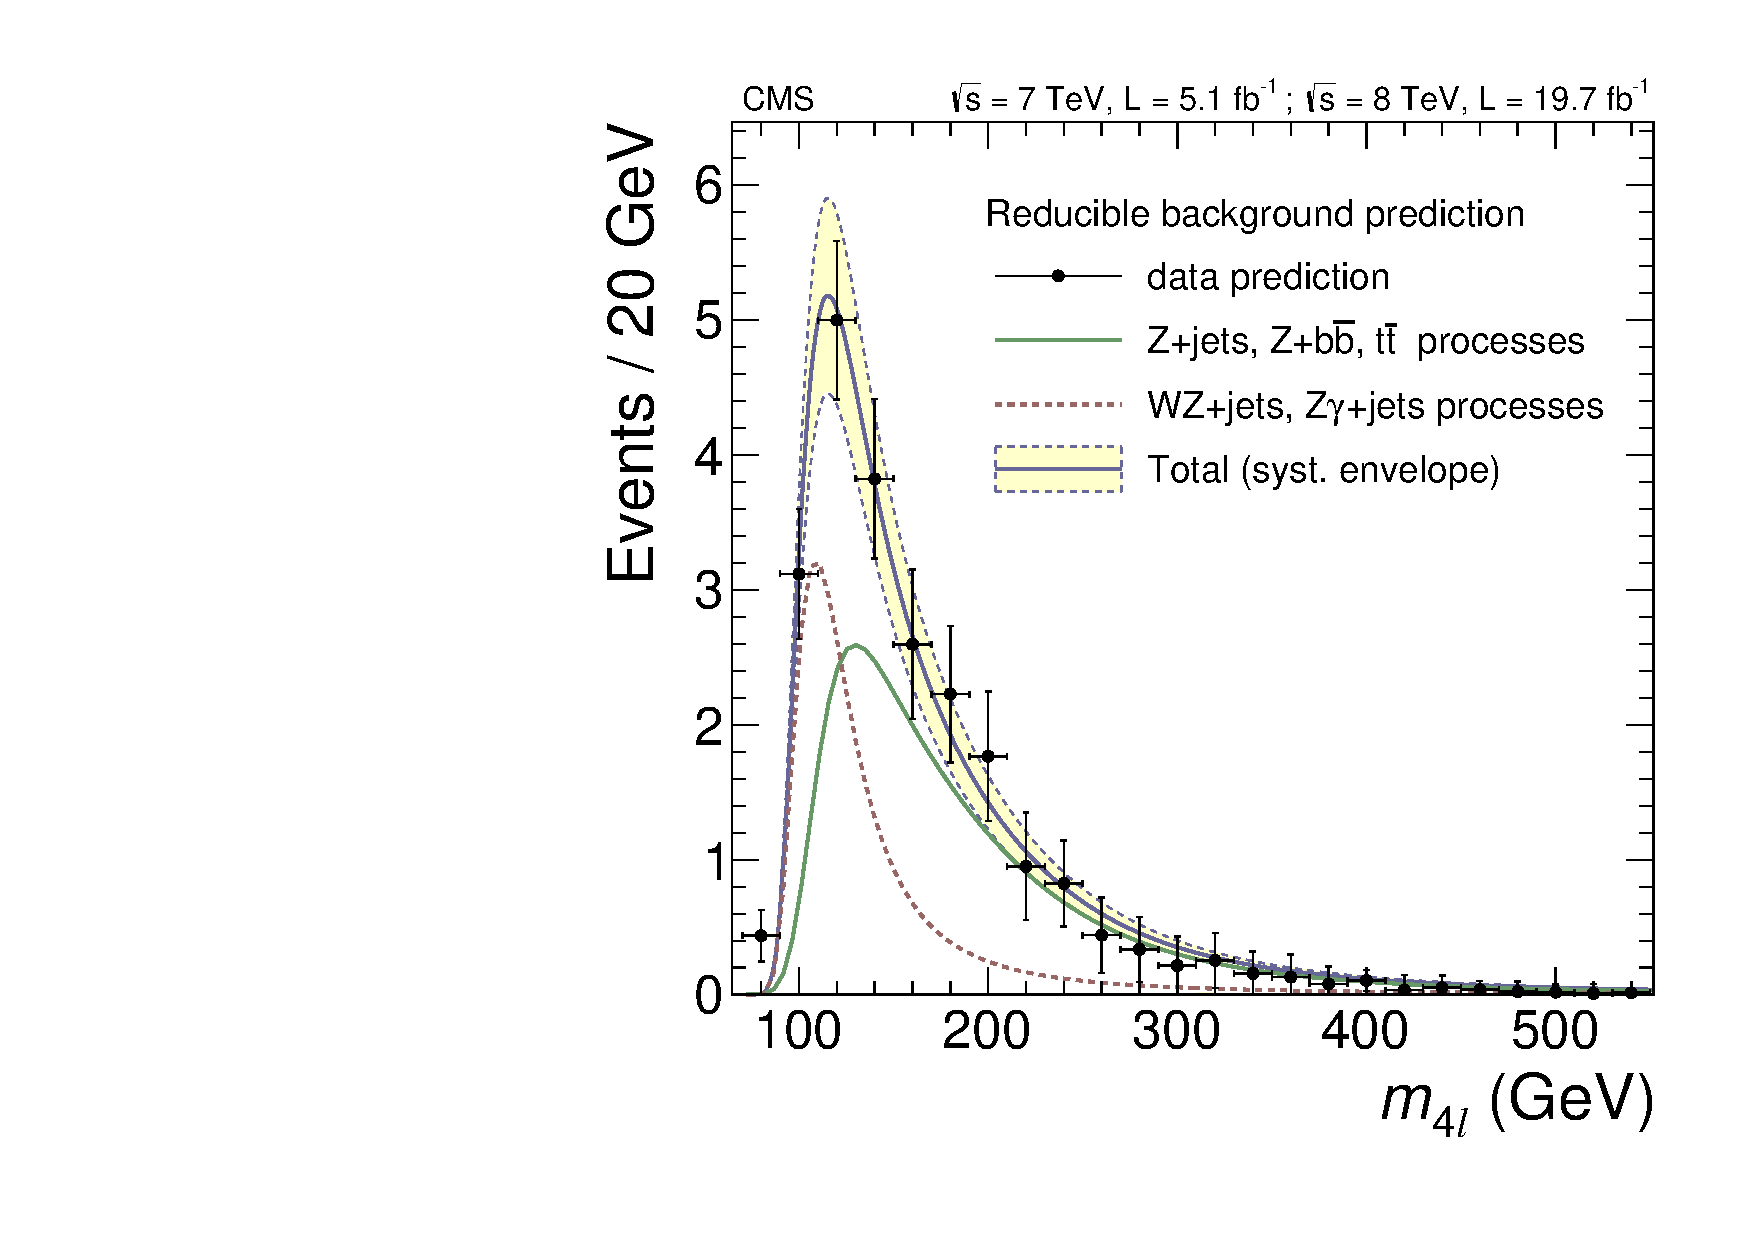
\includegraphics[width=.6\linewidth]{HiggsDiscovery/figures/PredictedComponentsSR_withData_PAPER.pdf}
\caption[Reducible Background Mass Shapes]{$m_{4l}$ Distributions for Reducible Background. Contributions from $Z$ + jets, $Z+b\bar{b}$, and $t\bar{t}$ come from 2P2F category (solid green) of OS control region. $WZ$ and $Z\gamma$ + jets come from 3P1F category (dashed red). Each contribution is fit separately to form full prediction (blue curve with yellow band indicating total uncertainty) compared to data (black dots).}
\label{fig:ZXMassShapes}
\end{center}
\end{figure}

For signals, the nominal mass shapes for the expected masses are found via MC simulation. For each Higgs mass simulated, the mass distribution is fit with a relativistic Breit-Wigner distribution\footnote{The Breit-Wigner distribution is commonly used in particle physics, representing the probability of generating an unstable propagator, like the $Z$ or Higgs, at a given energy.} convoluted with a double-sided Crystal Ball function\footnote{The Crystal Ball is a function that is used to give a gaussian distribution a long-tail with power-law behavior. A double-sided Crystal Ball applies this long tail on both sides of the gaussian. In particle physics, this is useful to account for energy leakage in the tails of probability distributions.} \cite{}. For $m_H < 400$ $\rm{GeV}$, this function is fit for all production mechanisms, jet categories, decay modes, and beam energy, where the normalization will vary by the expected cross section for that production or categorization. These normalizations have associated systematics (see Sec.~\ref{sec:ZZ4lSystematics}), while any shape uncertainties are minimal since the experimental mass resolution of the detector being much larger than the expected widths. Sample distributions for the signal are found in Fig.~\ref{fig:LMHiggsShape}.

\begin{figure}[htbp]
\begin{center}
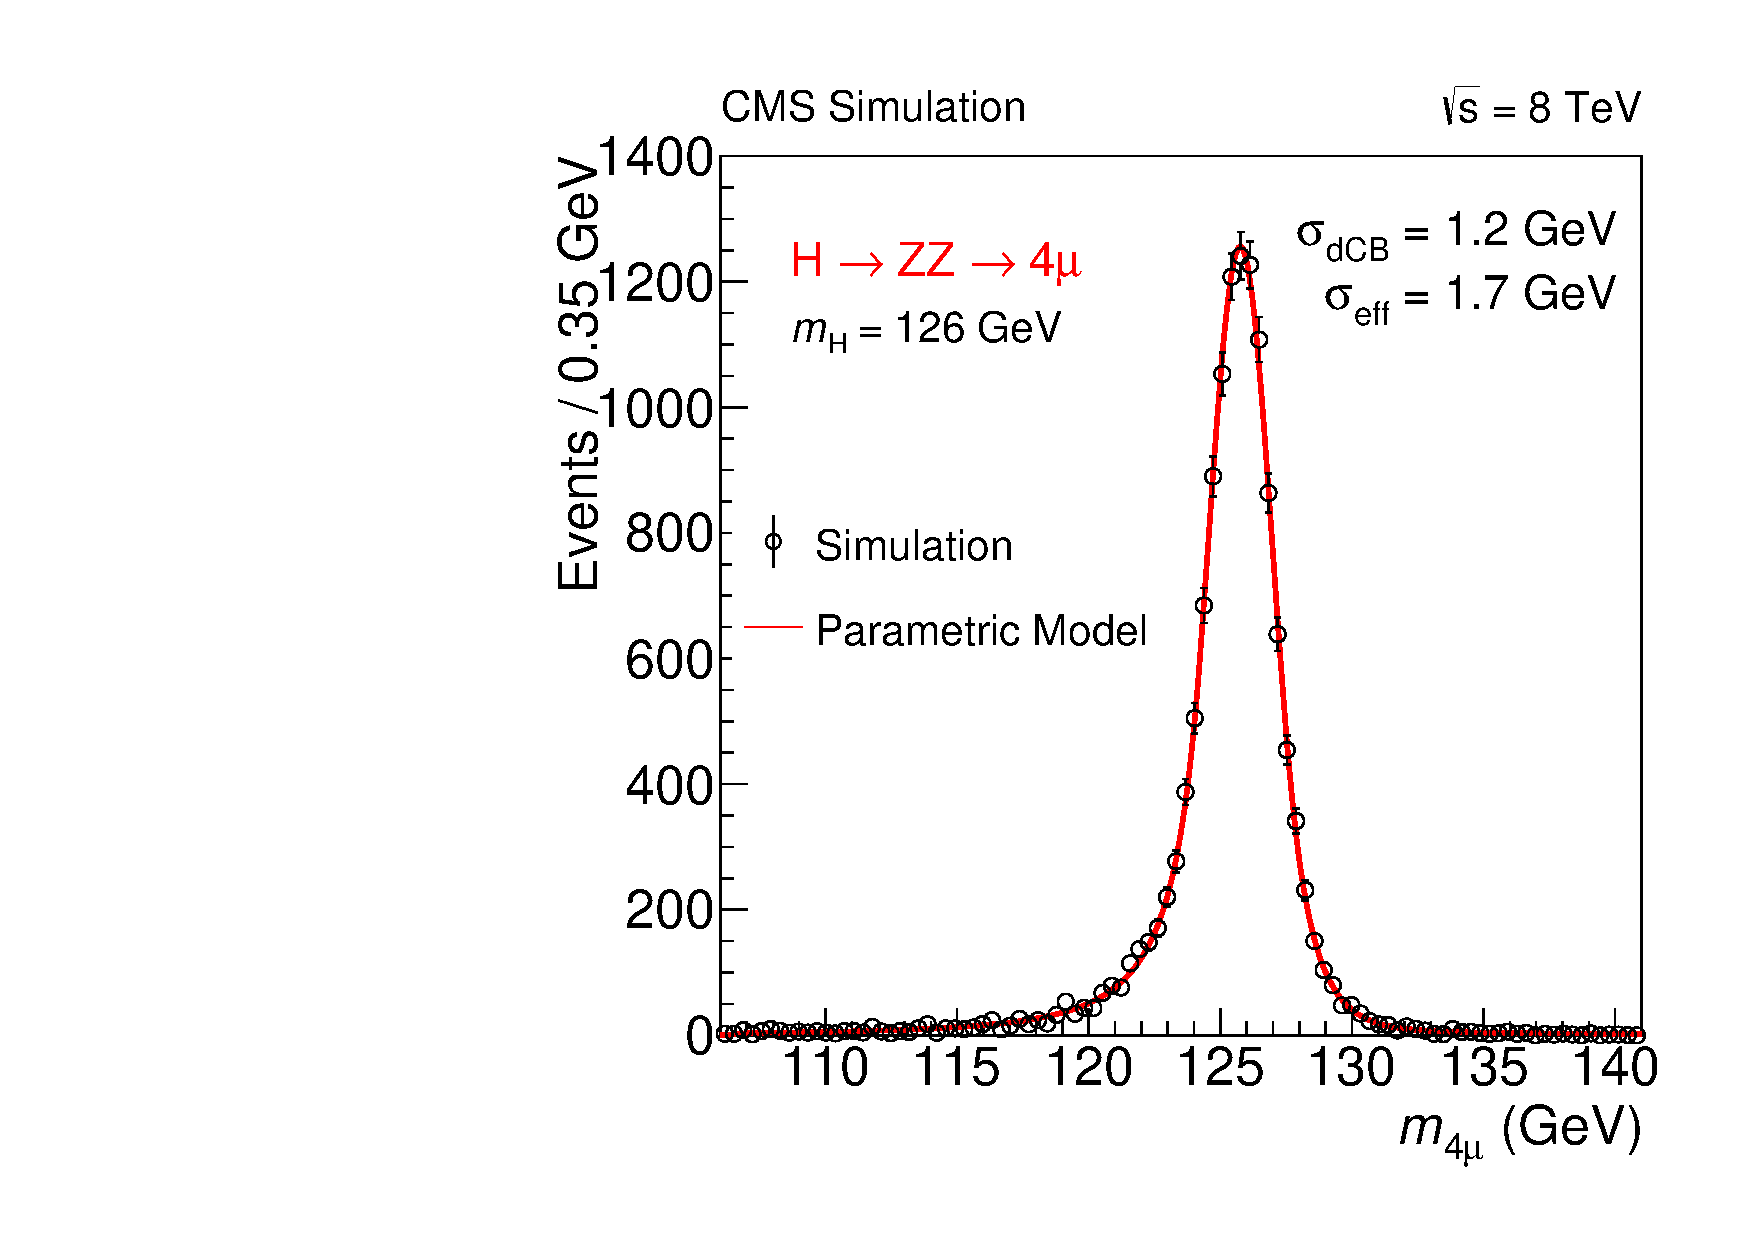
\includegraphics[width=.3\linewidth]{HiggsDiscovery/figures/fitM126_channel0.pdf}
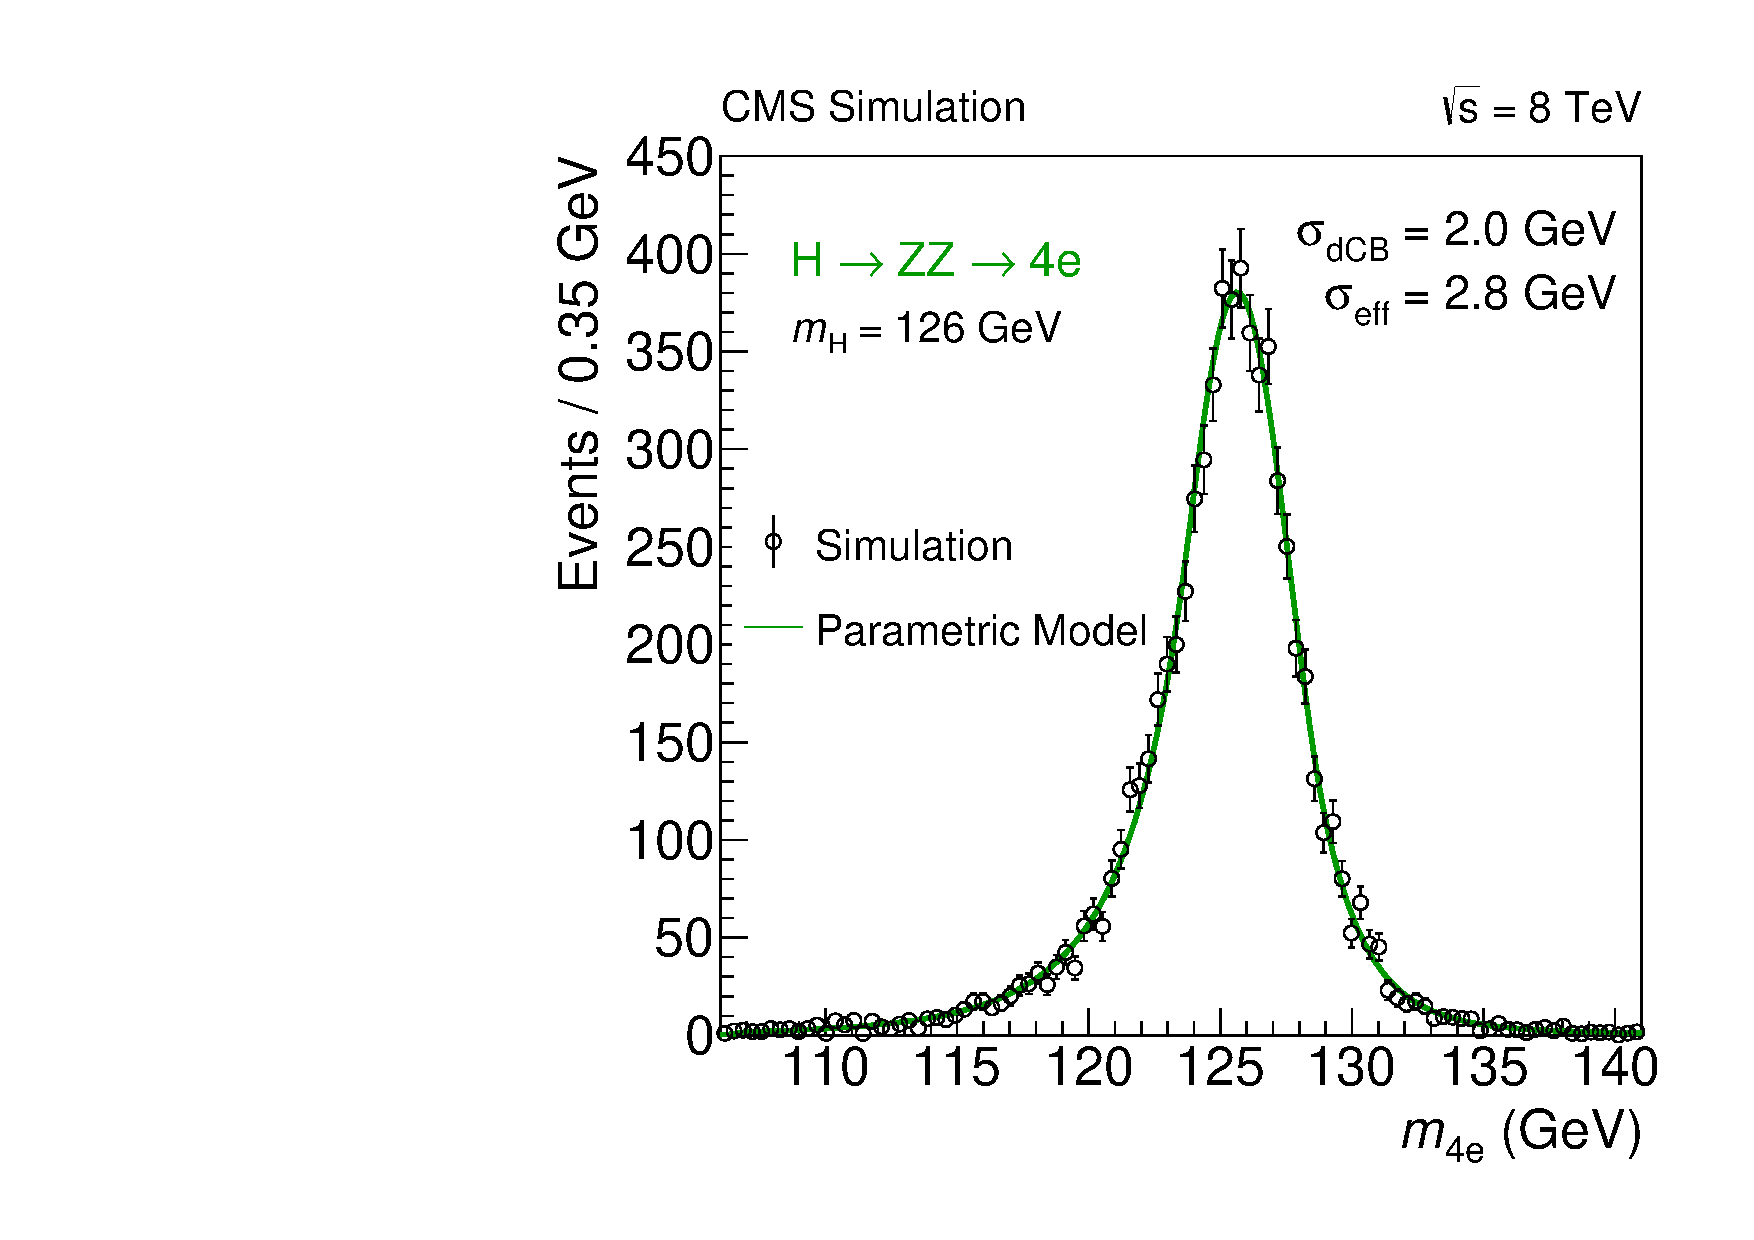
\includegraphics[width=.3\linewidth]{HiggsDiscovery/figures/fitM126_channel1.pdf}
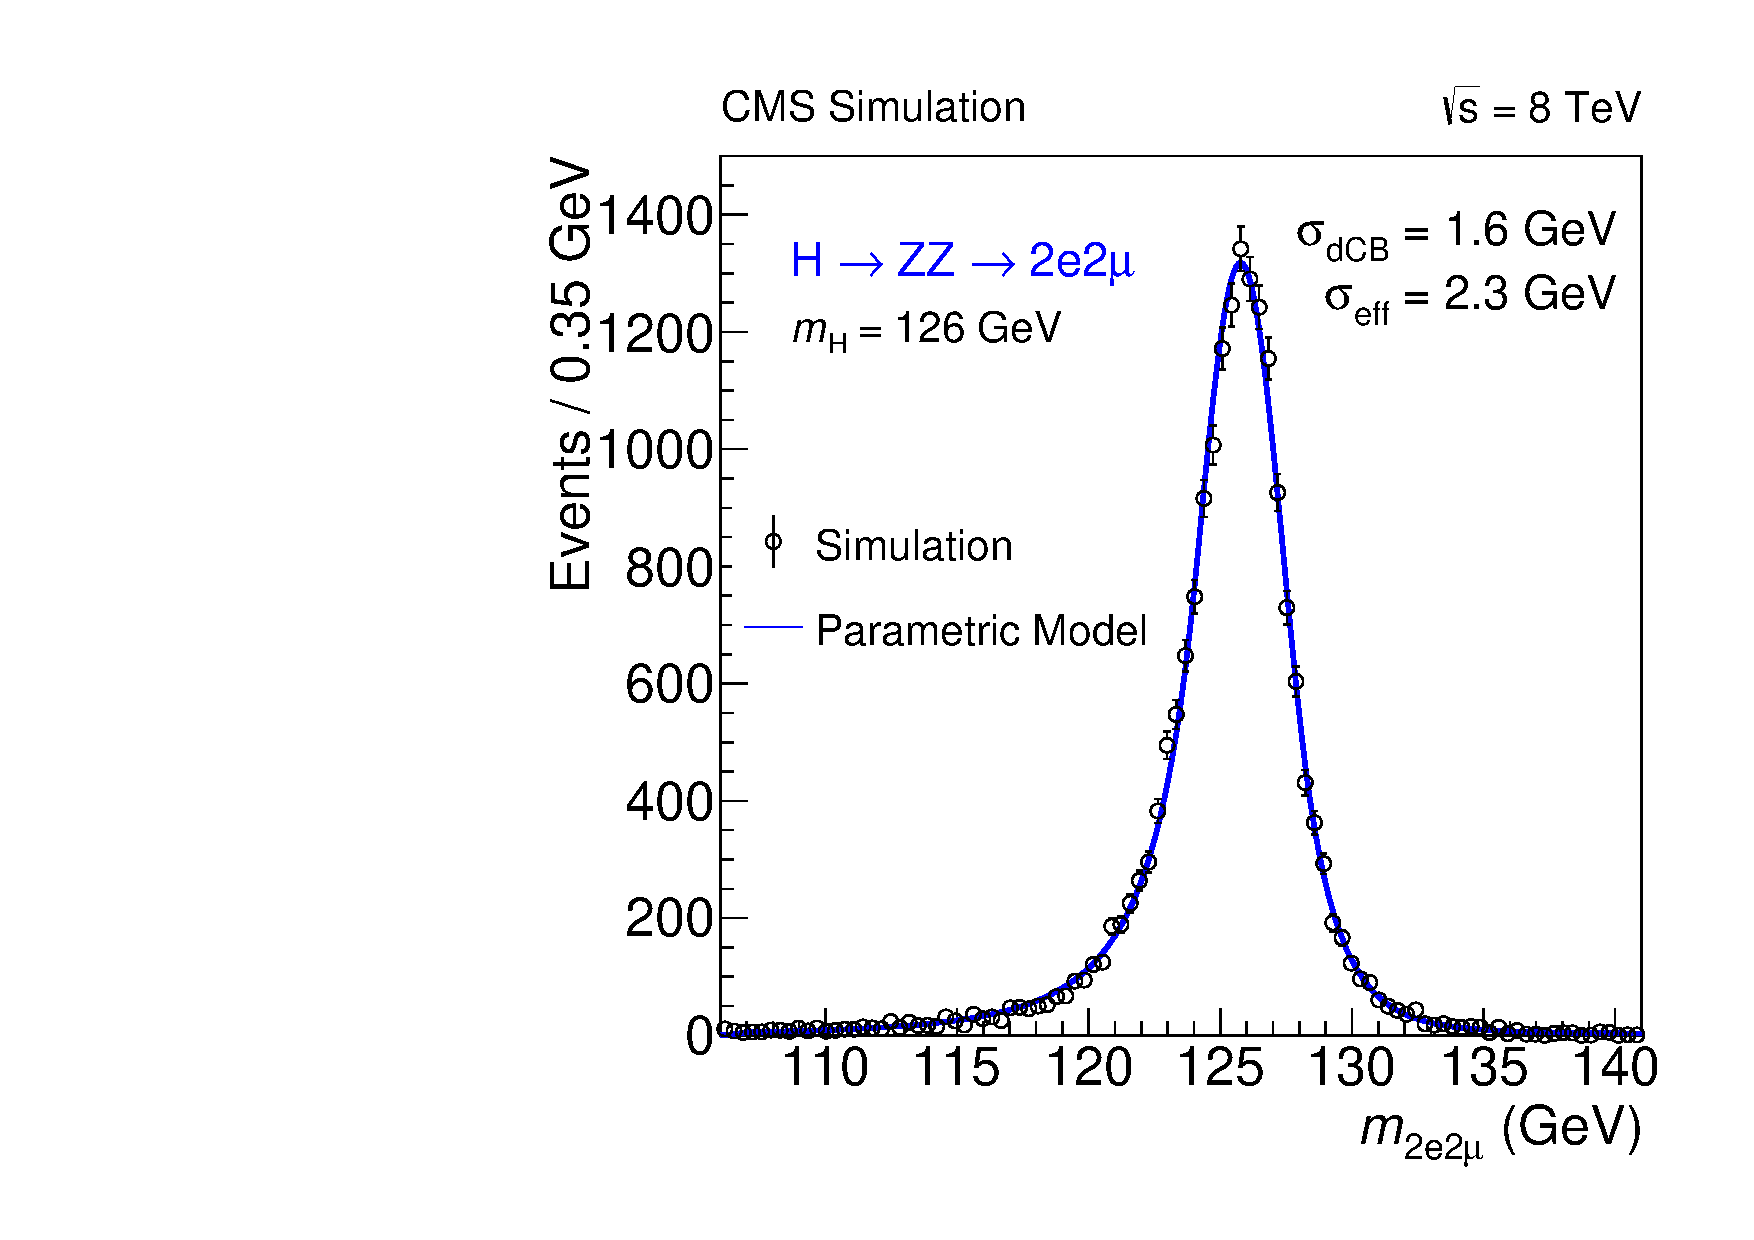
\includegraphics[width=.3\linewidth]{HiggsDiscovery/figures/fitM126_channel2.pdf}
\caption[Low Mass Higgs Signal Mass Shapes]{Sample Higgs signal $m_{4l}$ fits on MC simulation for $m_H=126$ $\rm{GeV}$ in ggF for $4\mu$ (left, red), $4e$ (middle, green), and $2e2\mu$ (right, blue) Each production method, beam energy, decay mode, and jet categorization has an independent fit for every mass point.}
\label{fig:LMHiggsShape}
\end{center}
\end{figure}

In the high mass region, $m_H \gtrsim 400$ $\rm{GeV}$, the mass shapes will change. As specified in Sec.~\ref{sec:ZZ4lMCandData}, the complex-pole scheme must be used and interference with the background is non-negligible, both of which enter into the signal $m_{4l}$ parameterizations via reweighting. After this reweighting, the Breit-Wigner constraint used for the lower masses is loosened by allowing the width to float such that it matches the MC distributions. Finally, instead of using the same mass shape for ggF and VBF, the shapes are found independently. The high mass $m_{4l}$ distributions have shape systematics arising from theoretical uncertainties in the applied corrections on top of any normalization systematics. Example high mass signal shapes with uncertainty bands are contained in Fig.~\ref{fig:HMHiggsShape}.

\begin{figure}[htbp]
\begin{center}
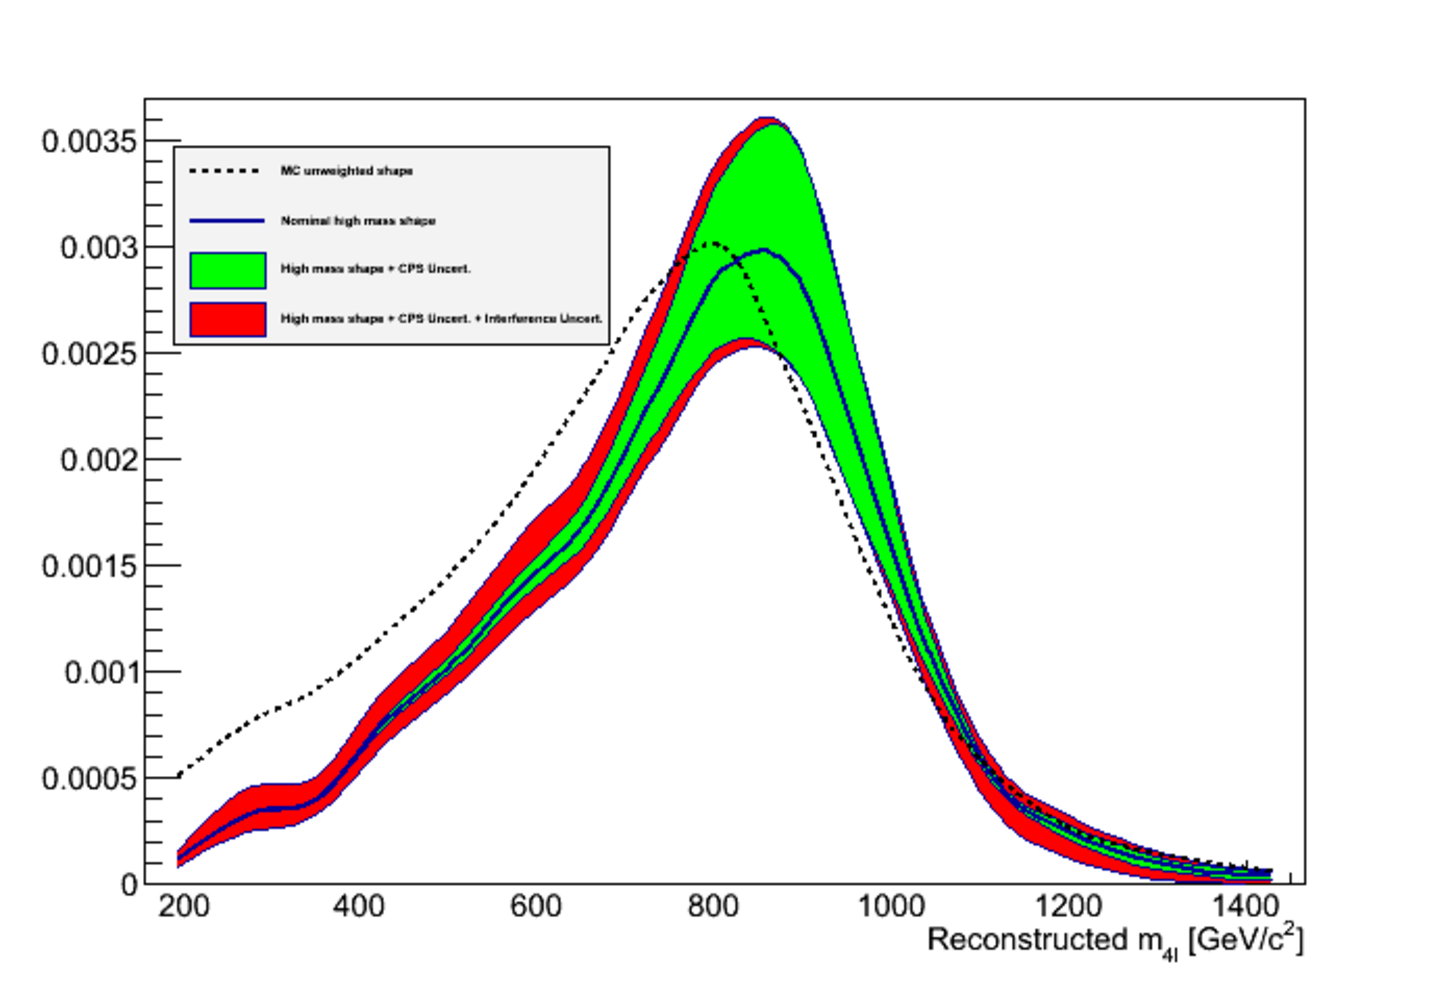
\includegraphics[width=.45\linewidth]{HiggsDiscovery/figures/H900_4mu_Reco_syst.pdf}
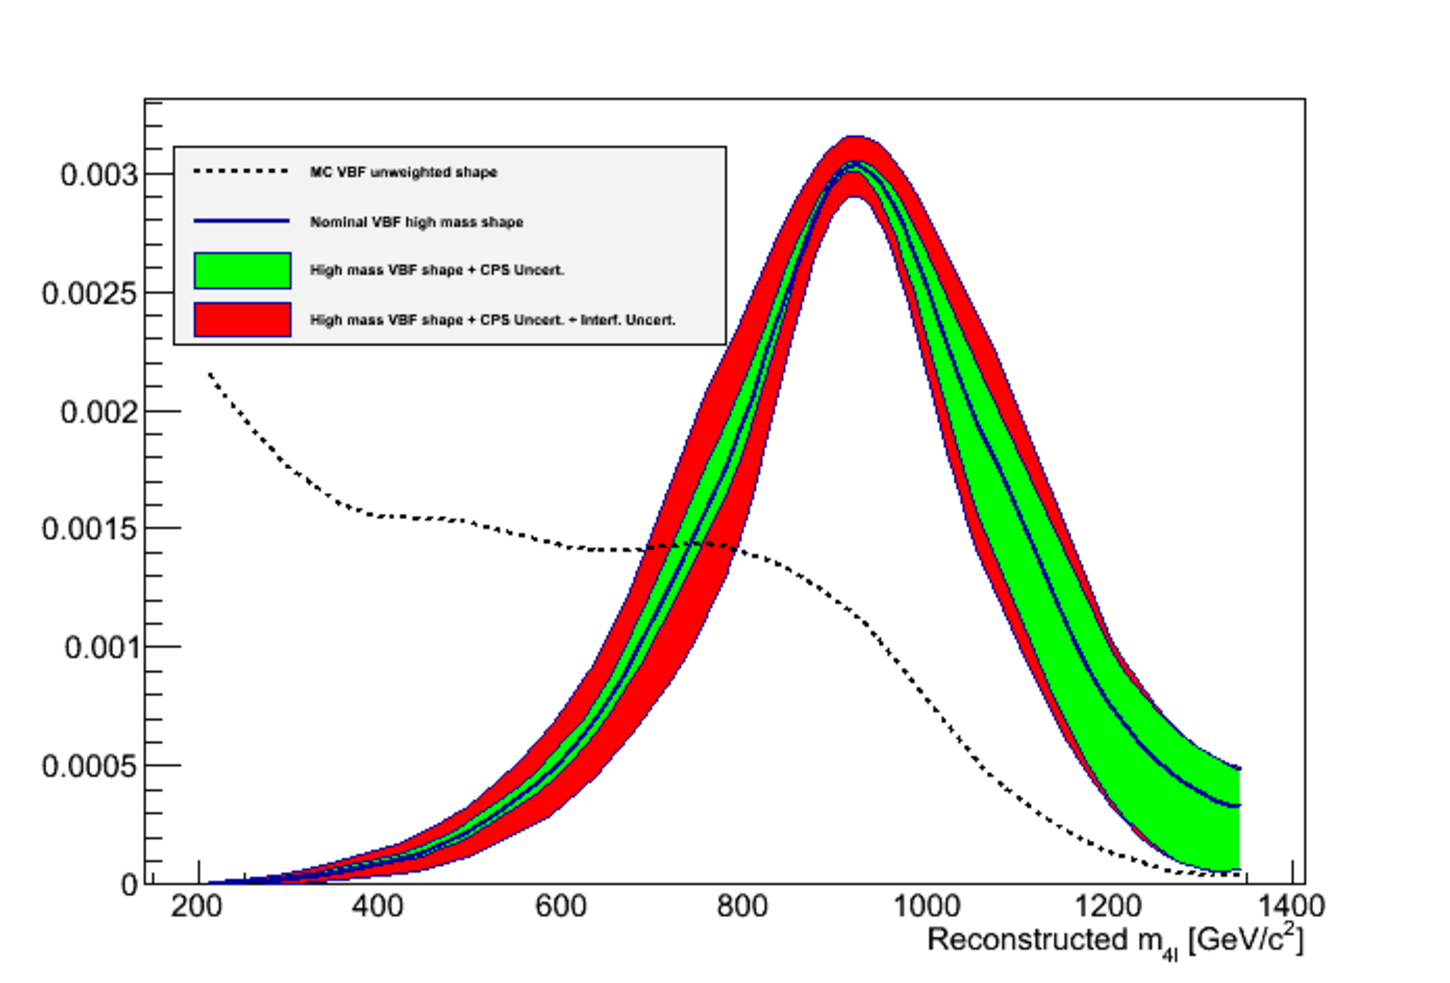
\includegraphics[width=.45\linewidth]{HiggsDiscovery/figures/VBFH900_4mu_Reco_syst.pdf}
\caption[High Mass Higgs Signal Mass Shapes]{Higgs signal $m_{4l}$ shapes for 900 $\rm{GeV}$ for ggF (left) and VBF (right). Dashed black line is shape directly from MC. Blue solid line accounts for complex-pole scheme reweighting and interference with backgrounds, where the red and green envelopes account for the uncertainty of reweighting.}
\label{fig:HMHiggsShape}
\end{center}
\end{figure}

These mass shapes can then be multiplied by the signal efficiencies, as discussed in Sec.~\ref{sec:ZZ4lSelection}, and the ratio for jet categorization, to be discussed in Sec.~\ref{sec:ZZ4lDjet}. This process gives the final yields for both the SM backgrounds and the Higgs signal as functions of $m_{4l}$ for any given Higgs mass to be evaluated.

\subsection{Kinematic Discriminant for Decay}
\label{sec:ZZ4lKD}

For any $4l$ event, the kinematic discriminant, $\mathcal{D}_{\rm{bkg}}^{\rm{kin}}$, can be constructed with the angular distributions of the decay. Eqn.~\ref{eq:MELADisc} defines the discriminant used, where the signal probability comes from the leading order {\tt JHUGen} matrix element and the background probability comes from the $q\bar{q}\rightarrow 4l$ LO matrix element found via {\tt MCFM}. Multiple sources for the matrix elements were tested with negligible differences. The relative normalization of the probabilities is tuned using a constant factor such that the total probability of signal plus background are equal above and below $\mathcal{D}_{\rm{bkg}}^{\rm{kin}} = 0.5$. No matrix element parameterization exists for $Z+X$, but the kinematic largely match those for $q\bar{q}\rightarrow 4l$ where a shape systematic is applied to account for any differences. Alternative methods using machine learning techniques, such as boosted decision trees or bayesian neural networks, show similar results to the matrix element approach. Two dimensional templates of $(m_{4l},\mathcal{D}_{\rm{bkg}}^{\rm{kin}})$ can be seen in Fig.~\ref{fig:MELATemplates}.

\begin{figure}[htbp]
\begin{center}
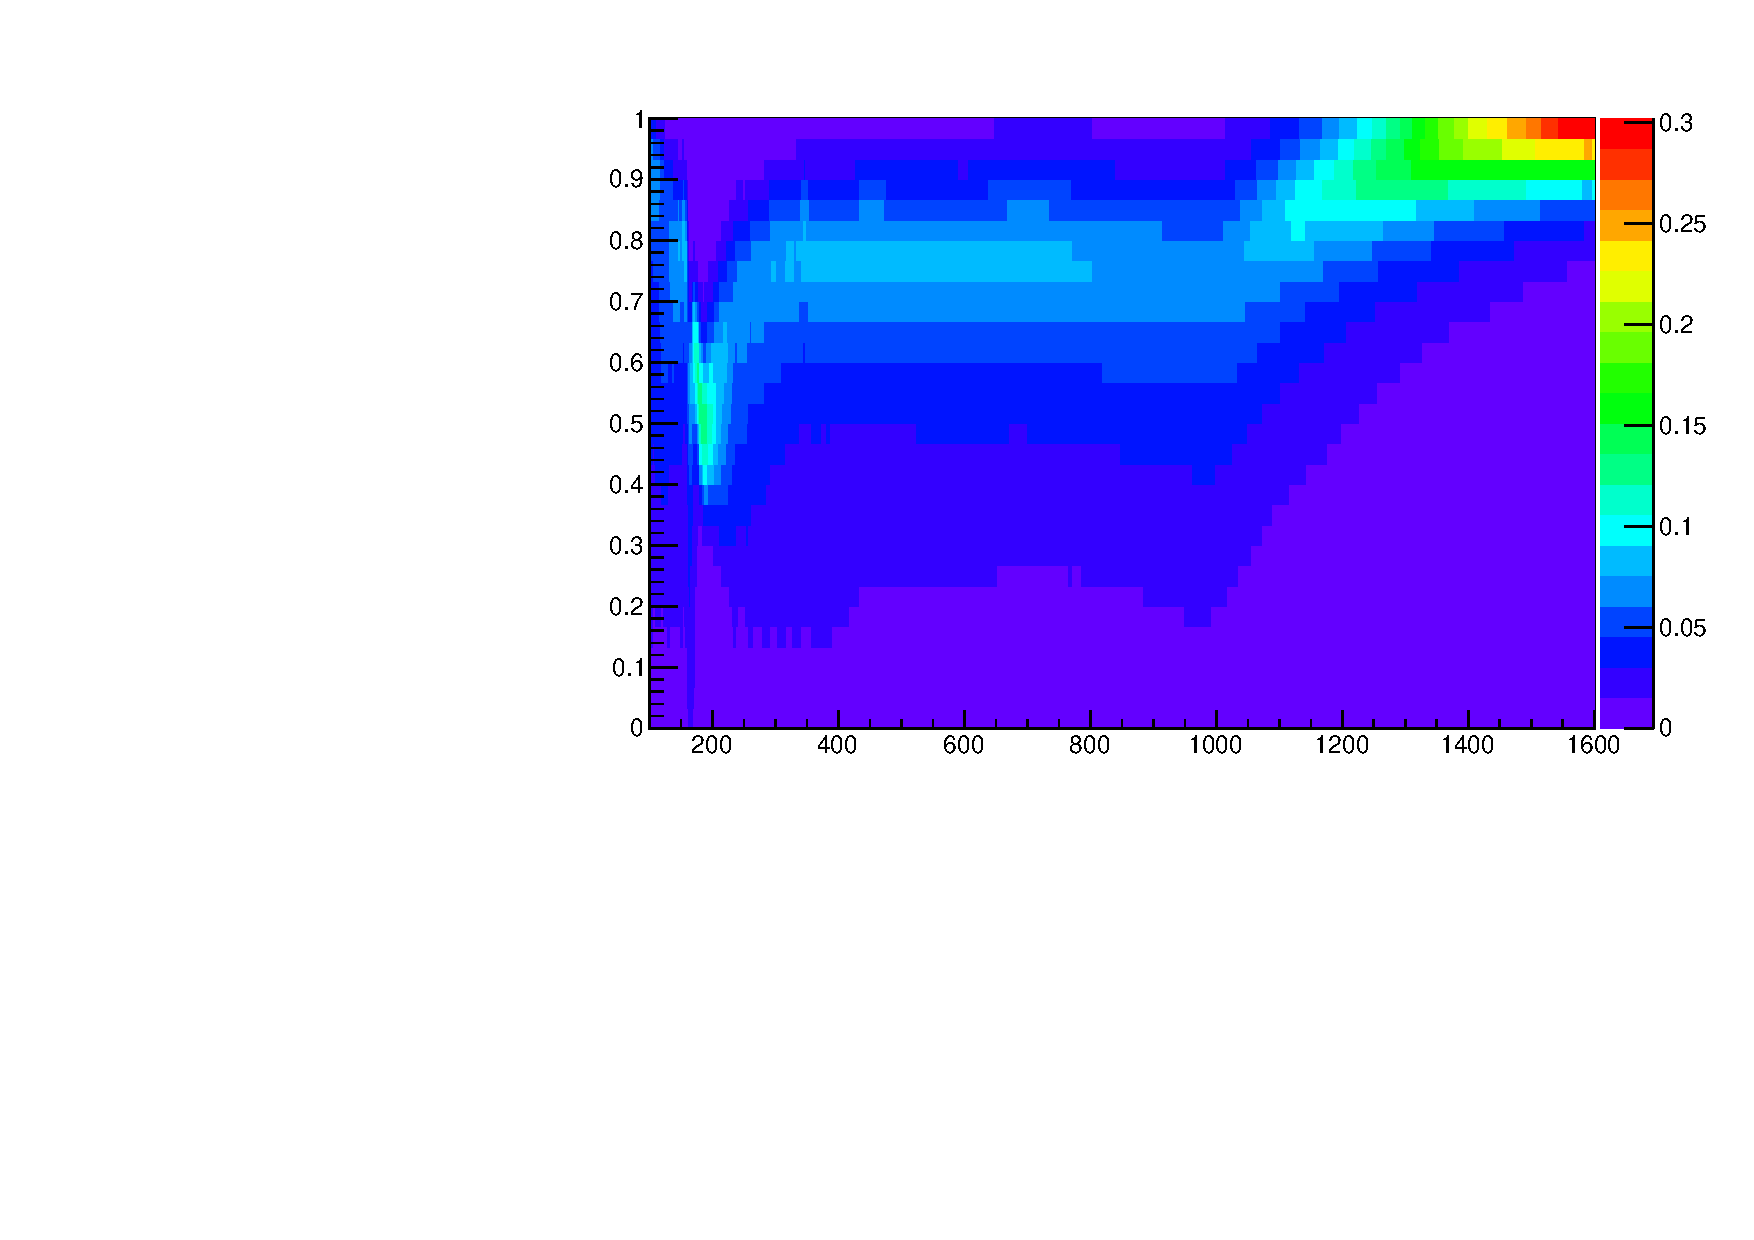
\includegraphics[width=.4\linewidth]{HiggsDiscovery/figures/Dsignal_2e2mu.pdf}
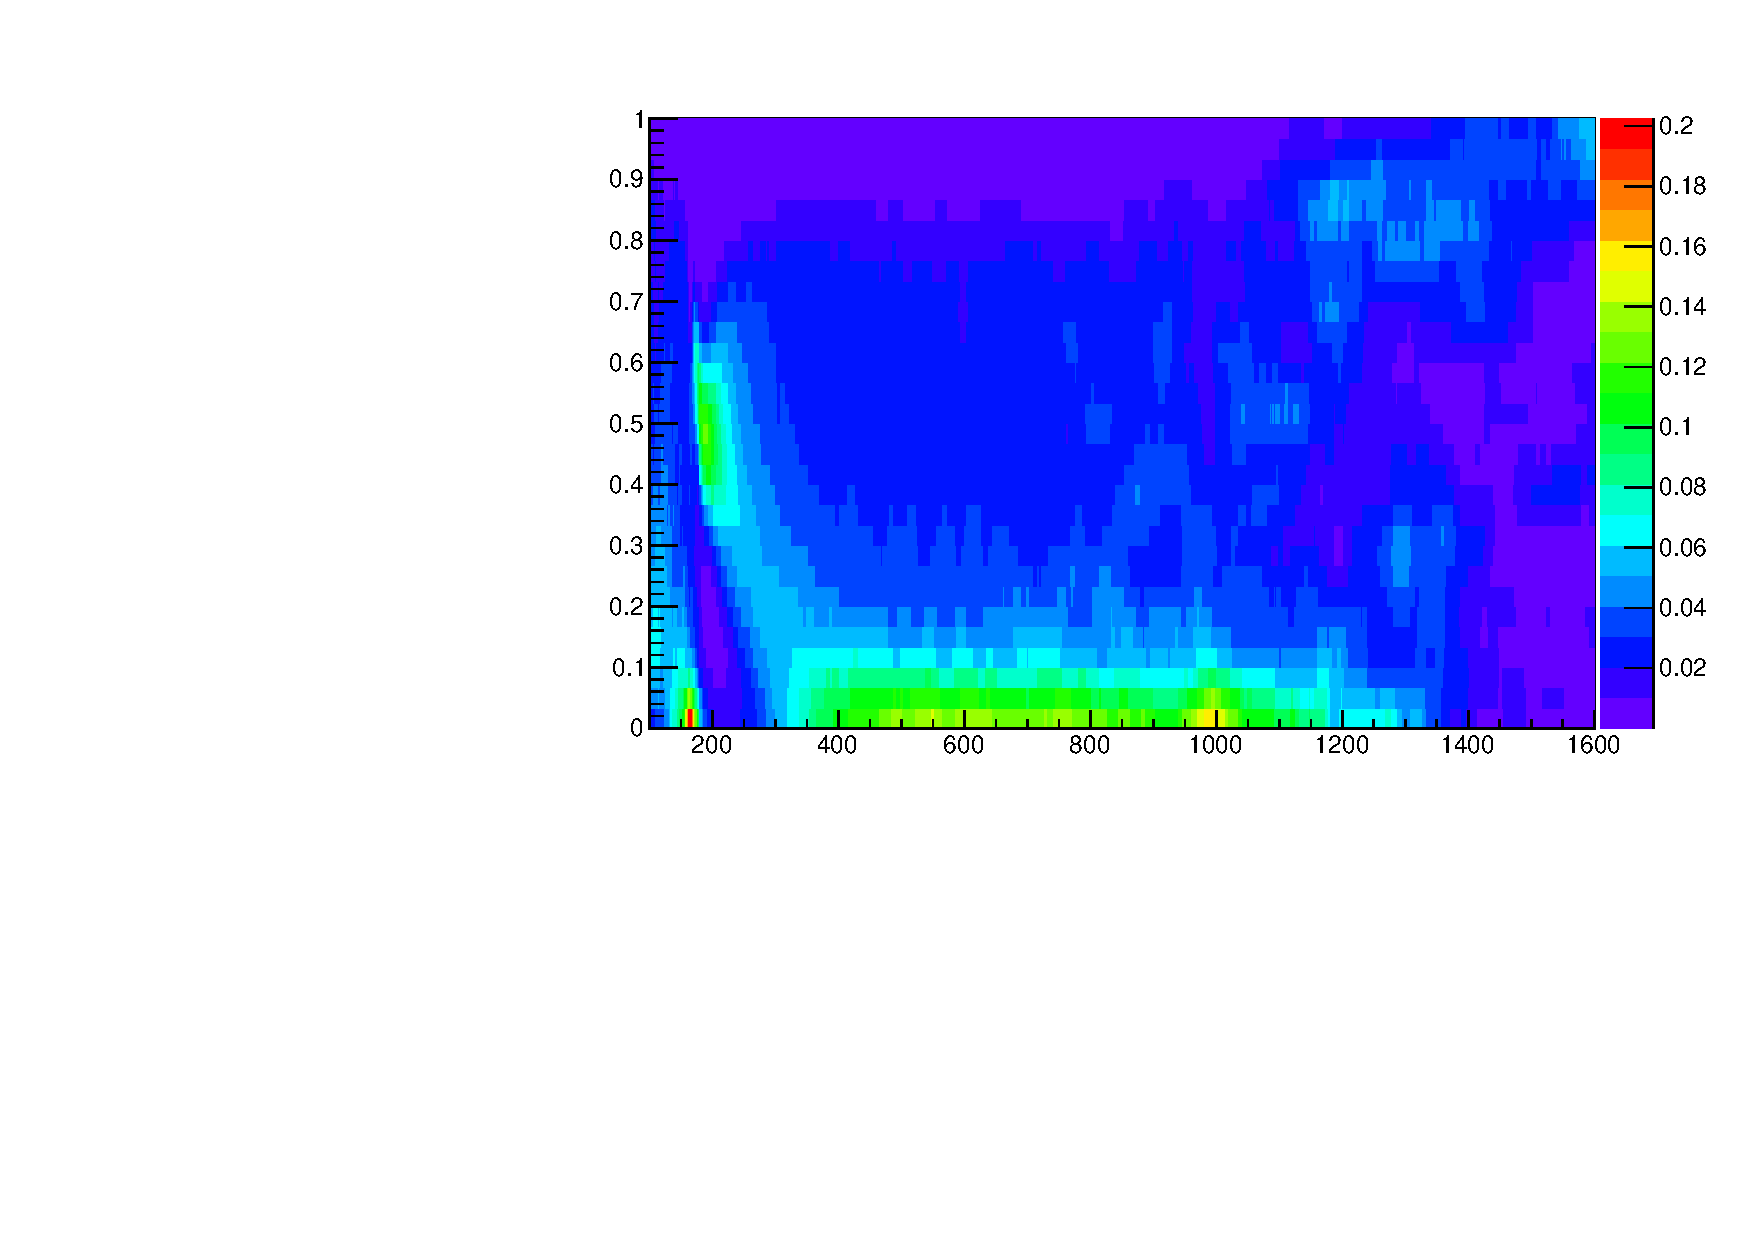
\includegraphics[width=.4\linewidth]{HiggsDiscovery/figures/Dbackground_qqZZ_2e2mu.pdf} \\
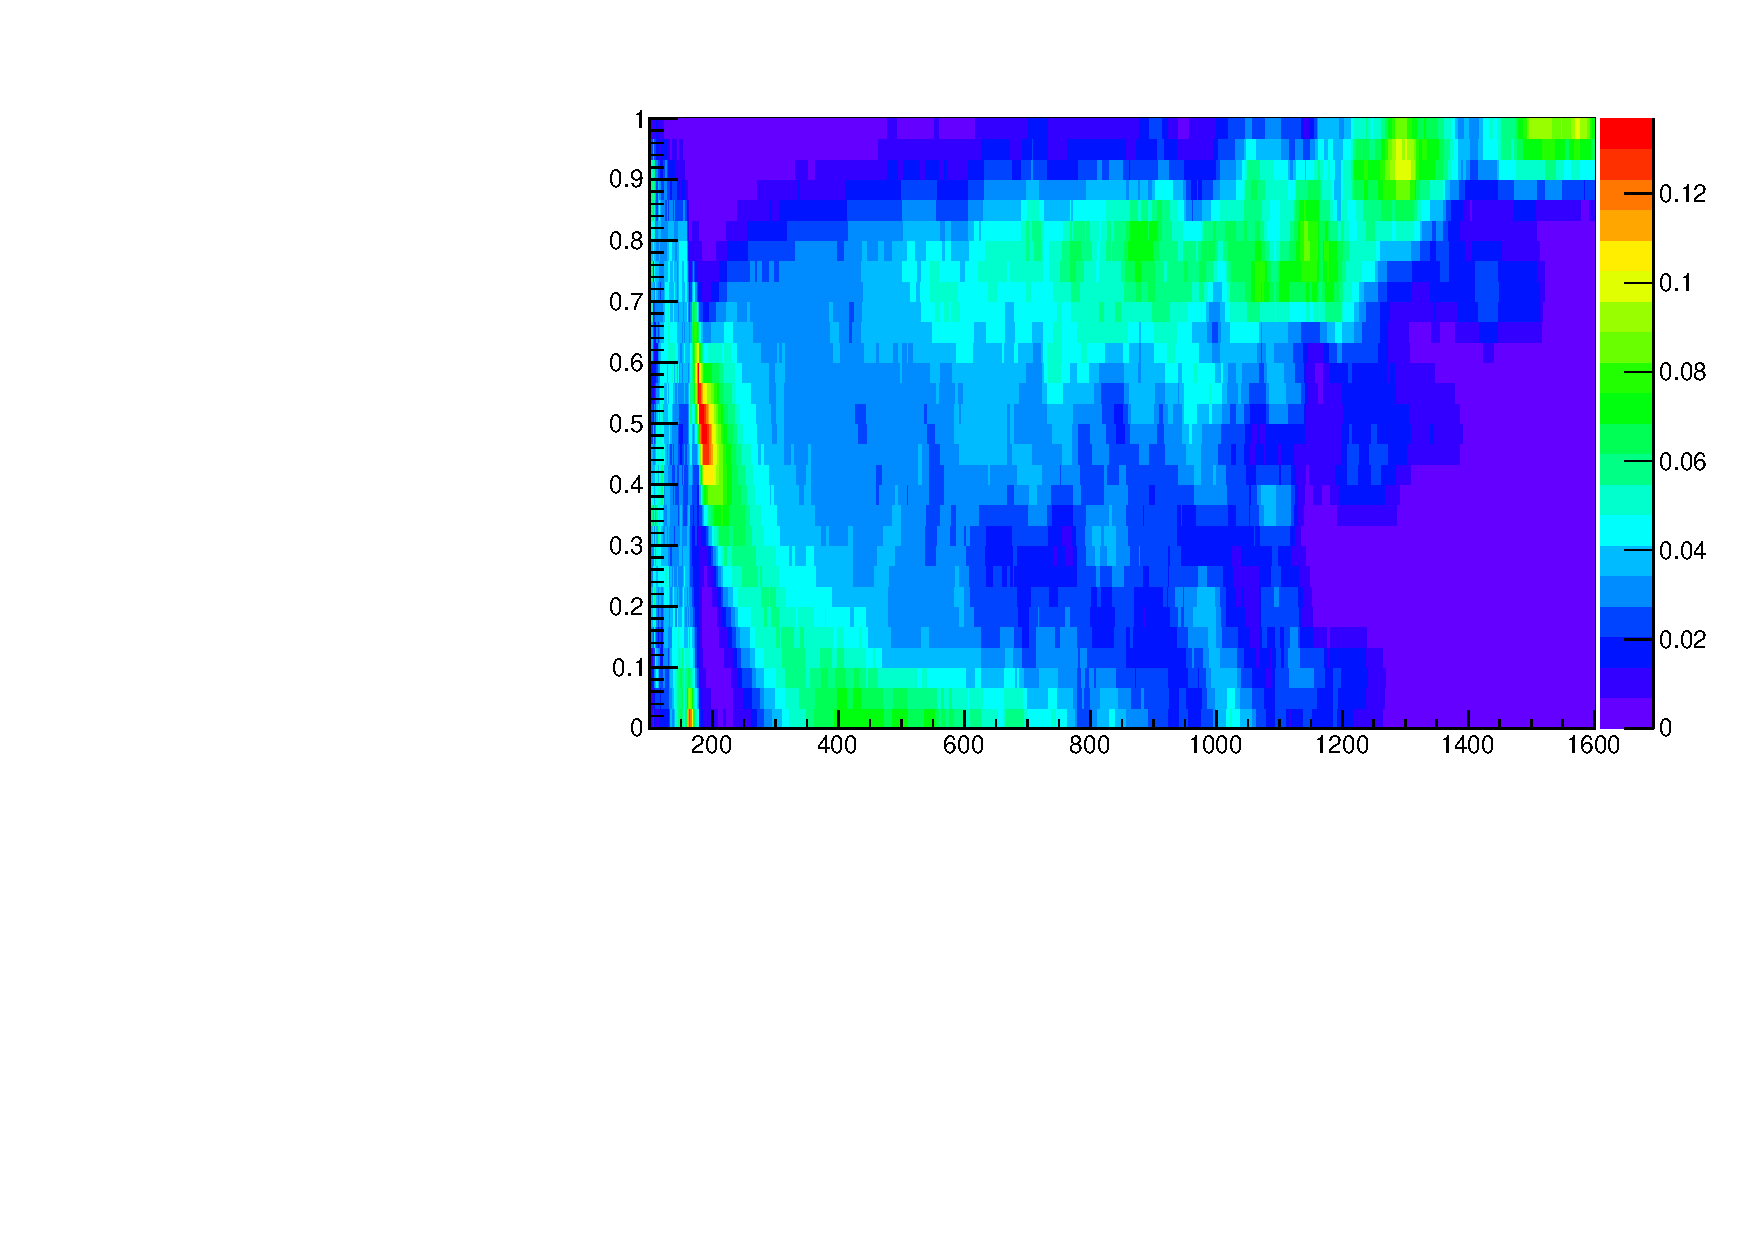
\includegraphics[width=.4\linewidth]{HiggsDiscovery/figures/Dbackground_ggZZ_2e2mu.pdf}
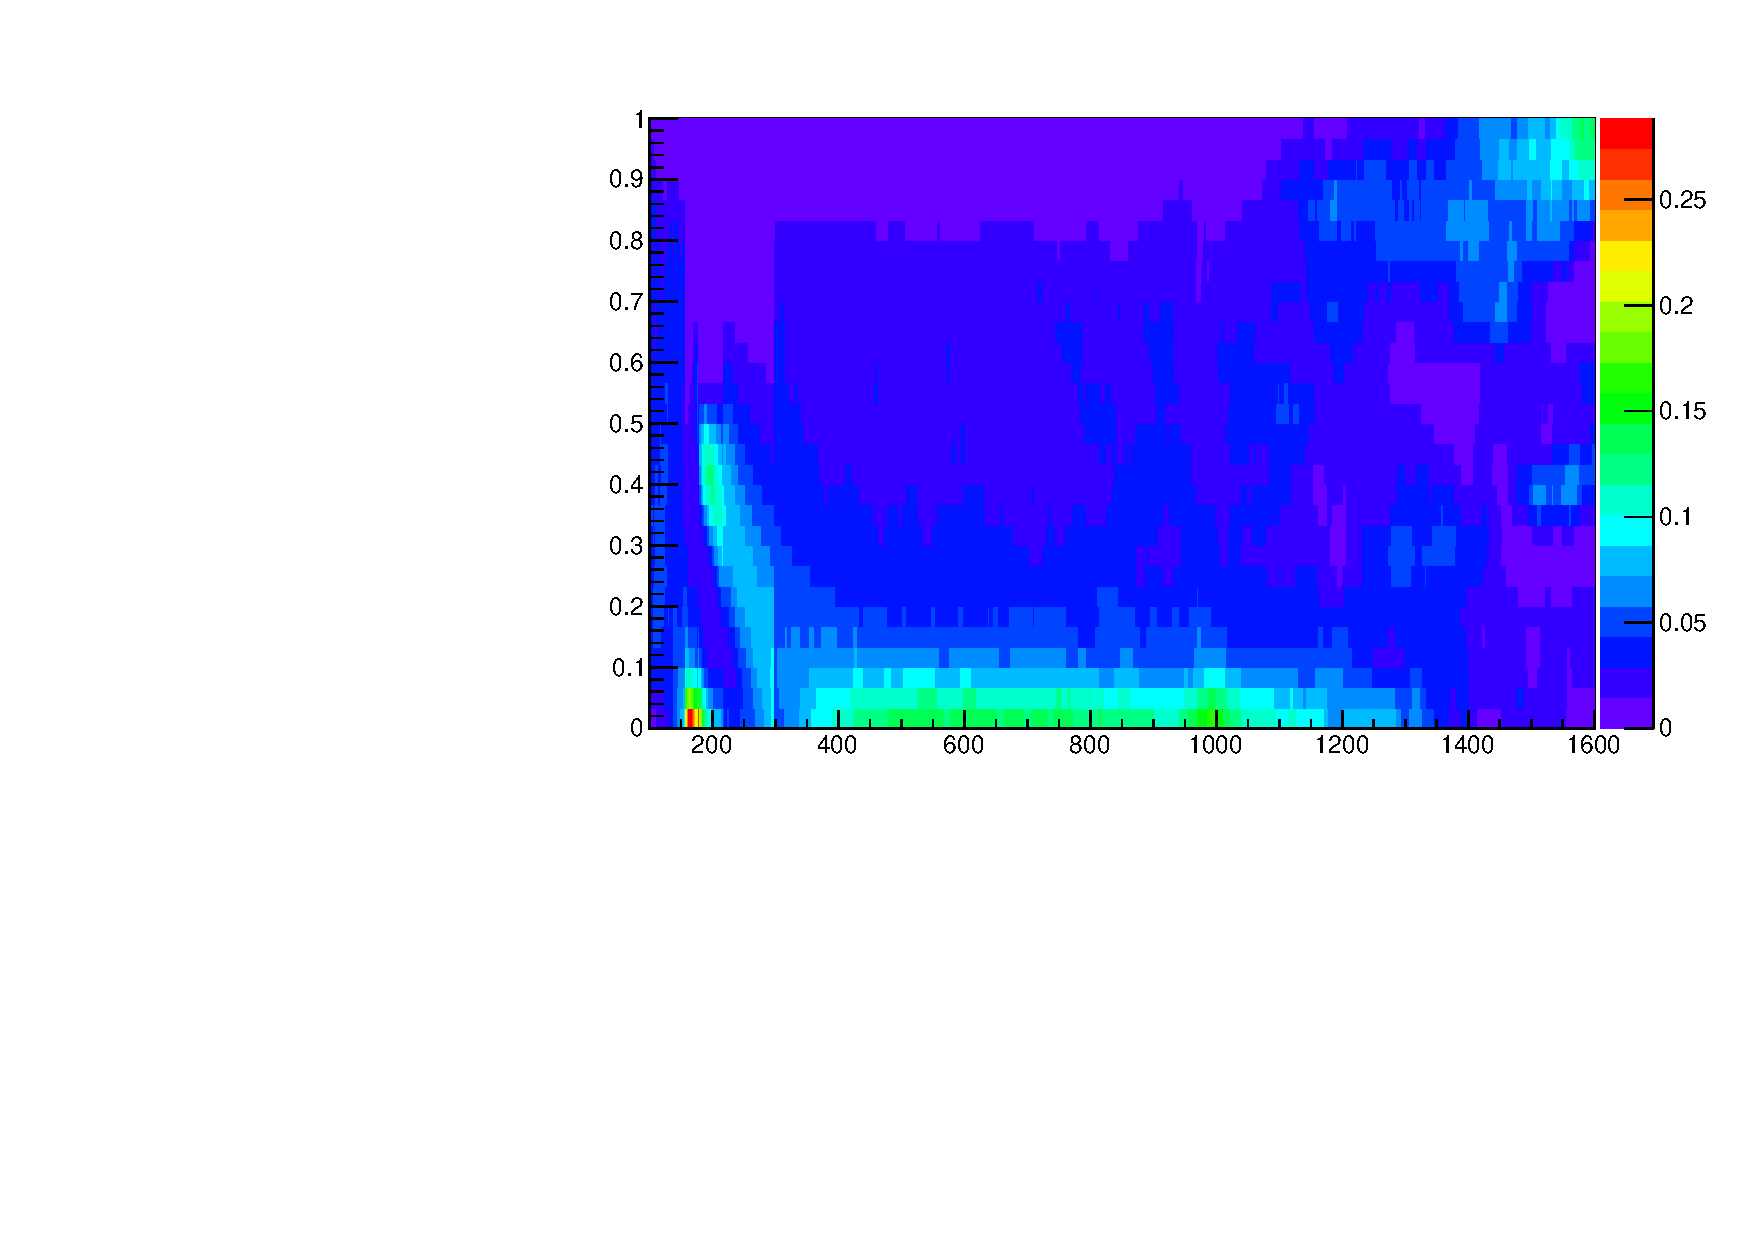
\includegraphics[width=.4\linewidth]{HiggsDiscovery/figures/Dbackground_ZX_2e2mu.pdf}
\caption[Templates of Kinematic Discriminant for $H \rightarrow ZZ \rightarrow 4l$]{Samples of $\mathcal{D}_{\rm{bkg}}^{\rm{kin}}$ v $m_{4l}$ templates for 8 $\rm{TeV}$ $2e2\mu$ Higgs signal(top left), $q\bar{q}\rightarrow ZZ$ (top right), $gg\rightarrow ZZ$ (bottom left), and $Z+X$ (bottom right) used in the analysis. Separate templates were made for $4e$, $4\mu$, and $2e2\mu$.}
\label{fig:MELATemplates}
\end{center}
\end{figure}

\subsection{Discriminating Production Mechanisms}
\label{sec:ZZ4lDjet}

As discussed in Sec.~\ref{sec:VBFVertex}, VBF events can be identified using the kinematics of the additional two jets over other production mechanisms or backgrounds. In that vein, after selection, events are categorized by their number of jets. The \textit{dijet} category encapsulates all events with at least two jets meeting the definitions in Sec.~\ref{sec:zz4lJets}. All other selected events fall into the \textit{non-dijet} category. On top of the signal selection efficiency, the dijet ratio is constructed as a function of $m_H$ (Figs.~\ref{fig:DijetRatioggHqqH} and~\ref{fig:DijetRatioAss}) to determine the expected number of expected signal and background events in a particular category and thus enters into the $m_{4l}$ distributions for each jet category.

\begin{figure}[htbp]
\begin{center}
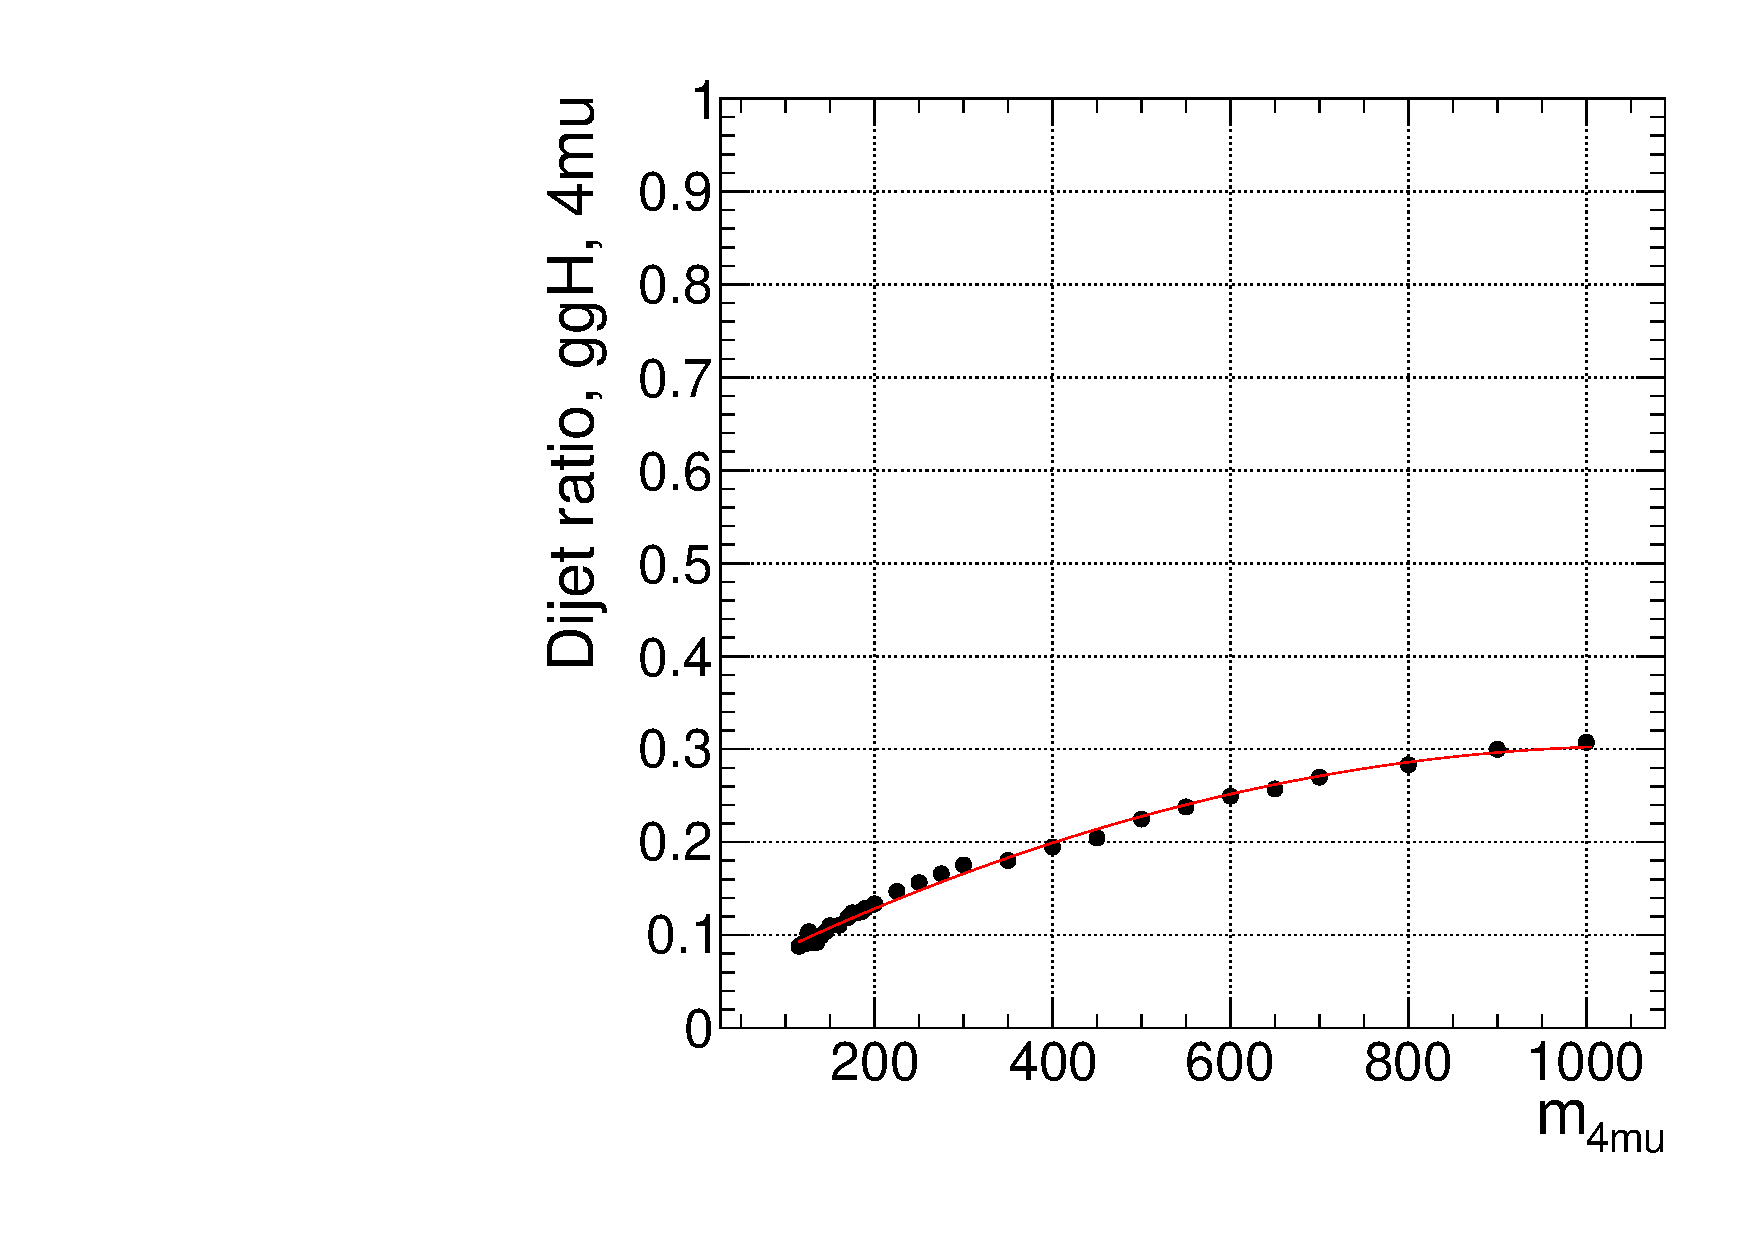
\includegraphics[width=.3\linewidth]{HiggsDiscovery/figures/eff_ggH_4mu_ratio.pdf}
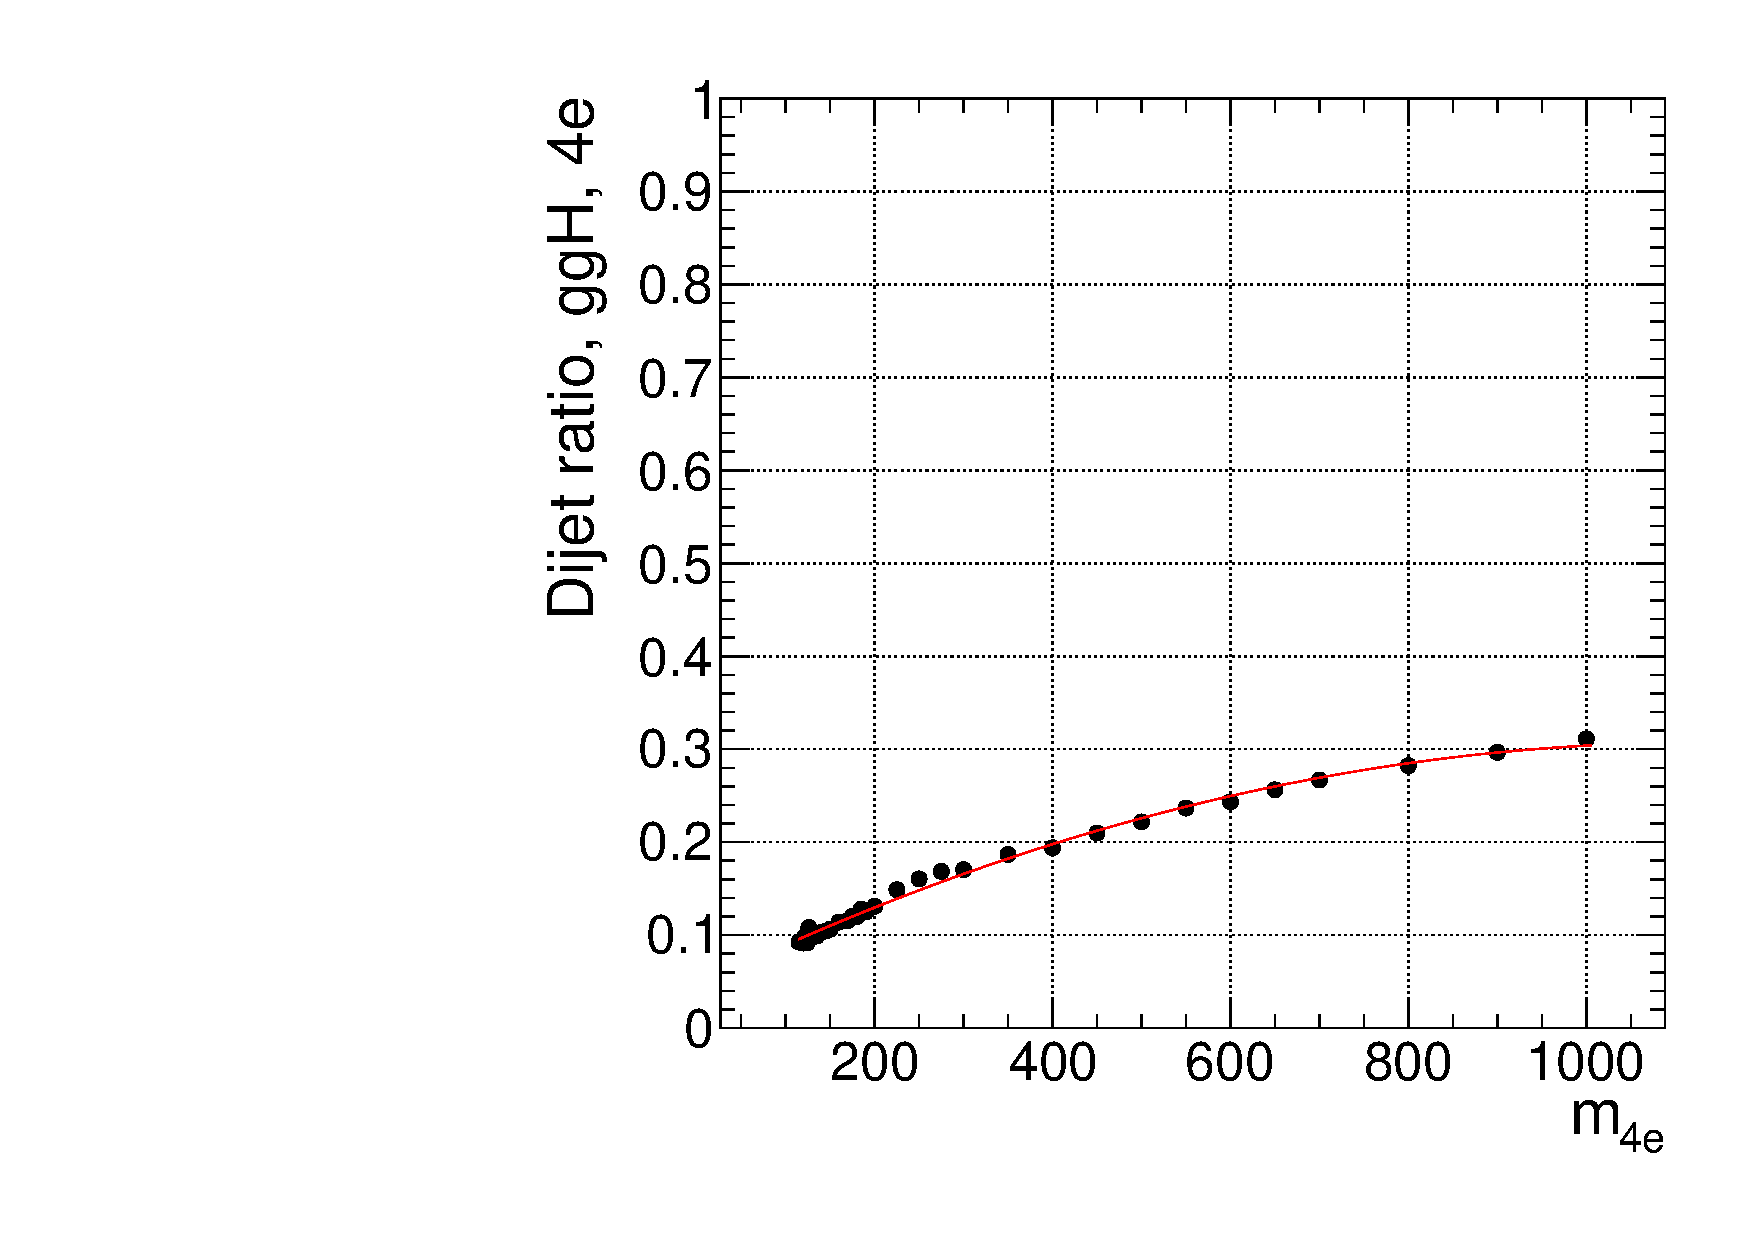
\includegraphics[width=.3\linewidth]{HiggsDiscovery/figures/eff_ggH_4e_ratio.pdf}
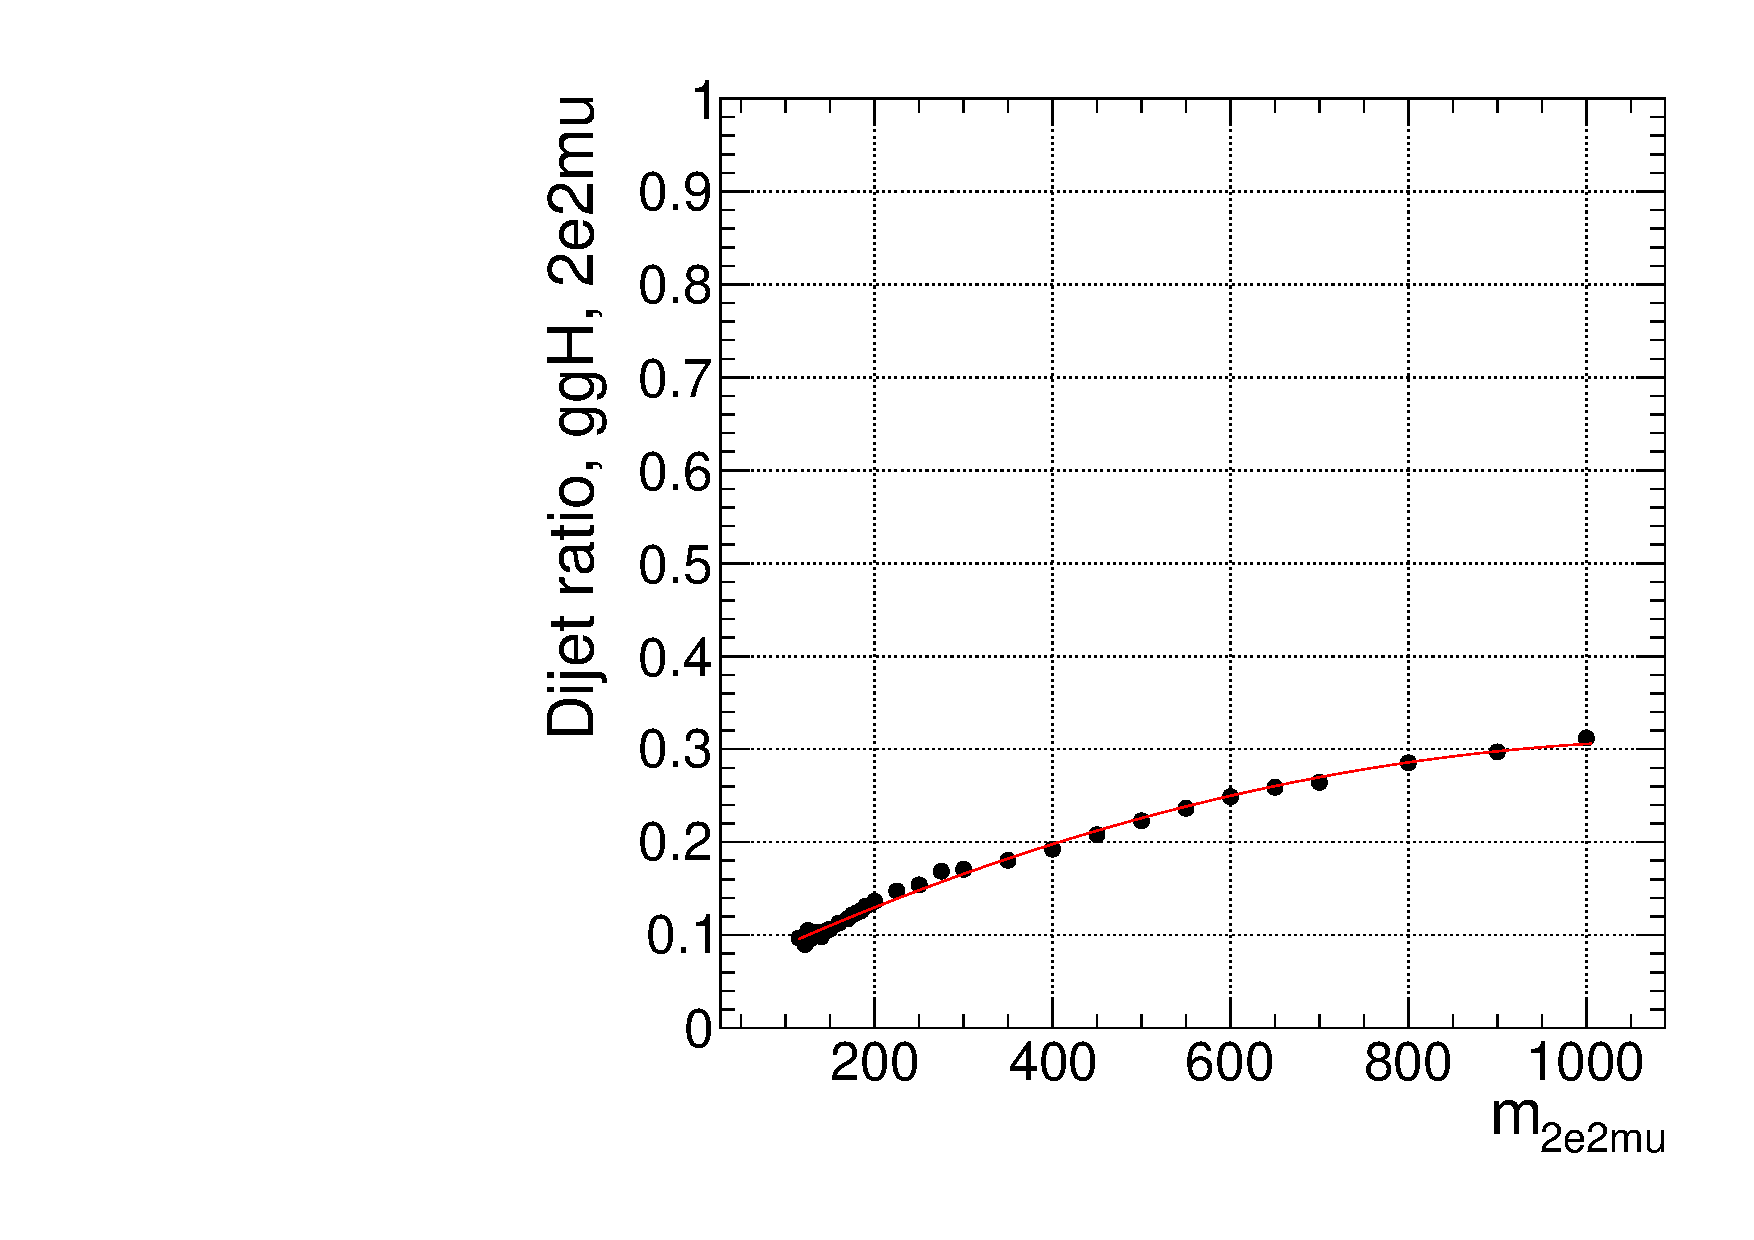
\includegraphics[width=.3\linewidth]{HiggsDiscovery/figures/eff_ggH_2e2mu_ratio.pdf} \\
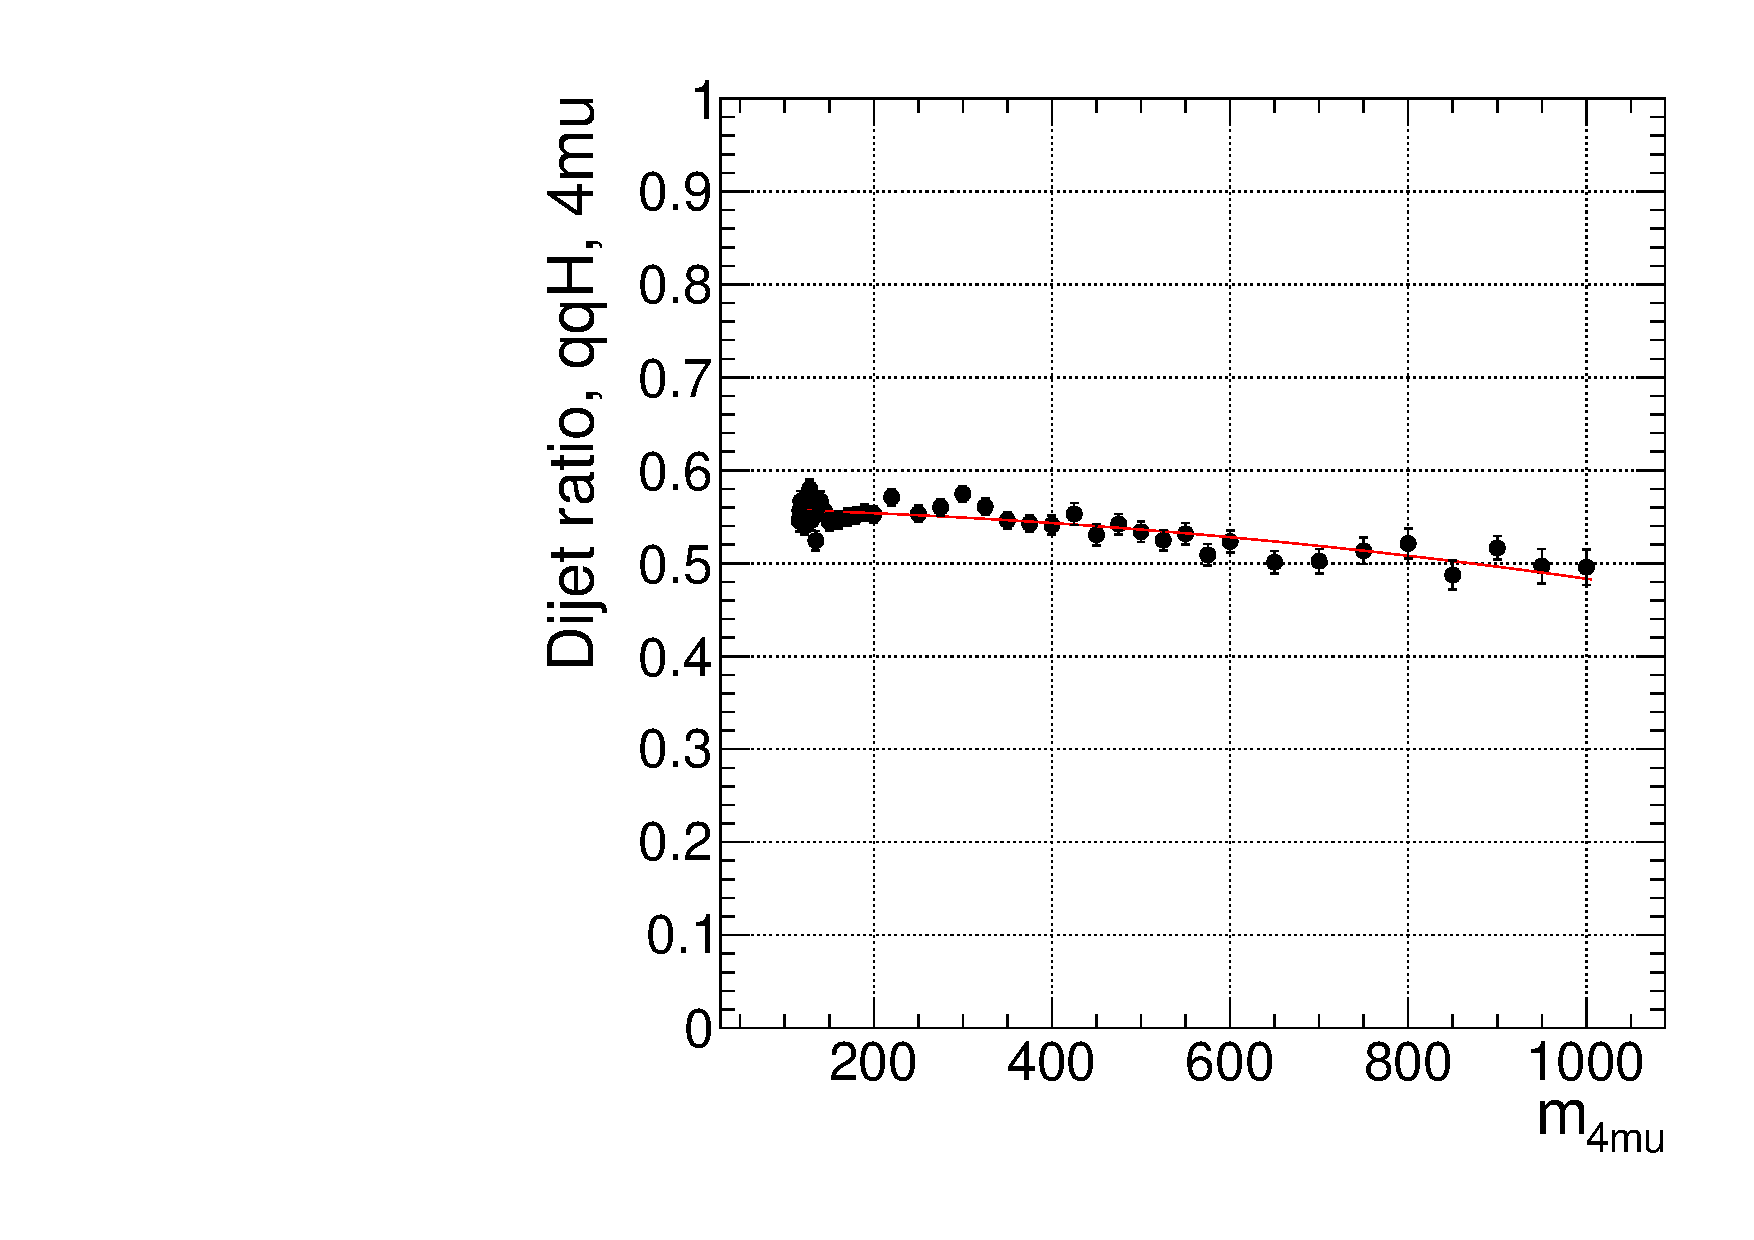
\includegraphics[width=.3\linewidth]{HiggsDiscovery/figures/eff_qqH_4mu_ratio.pdf}
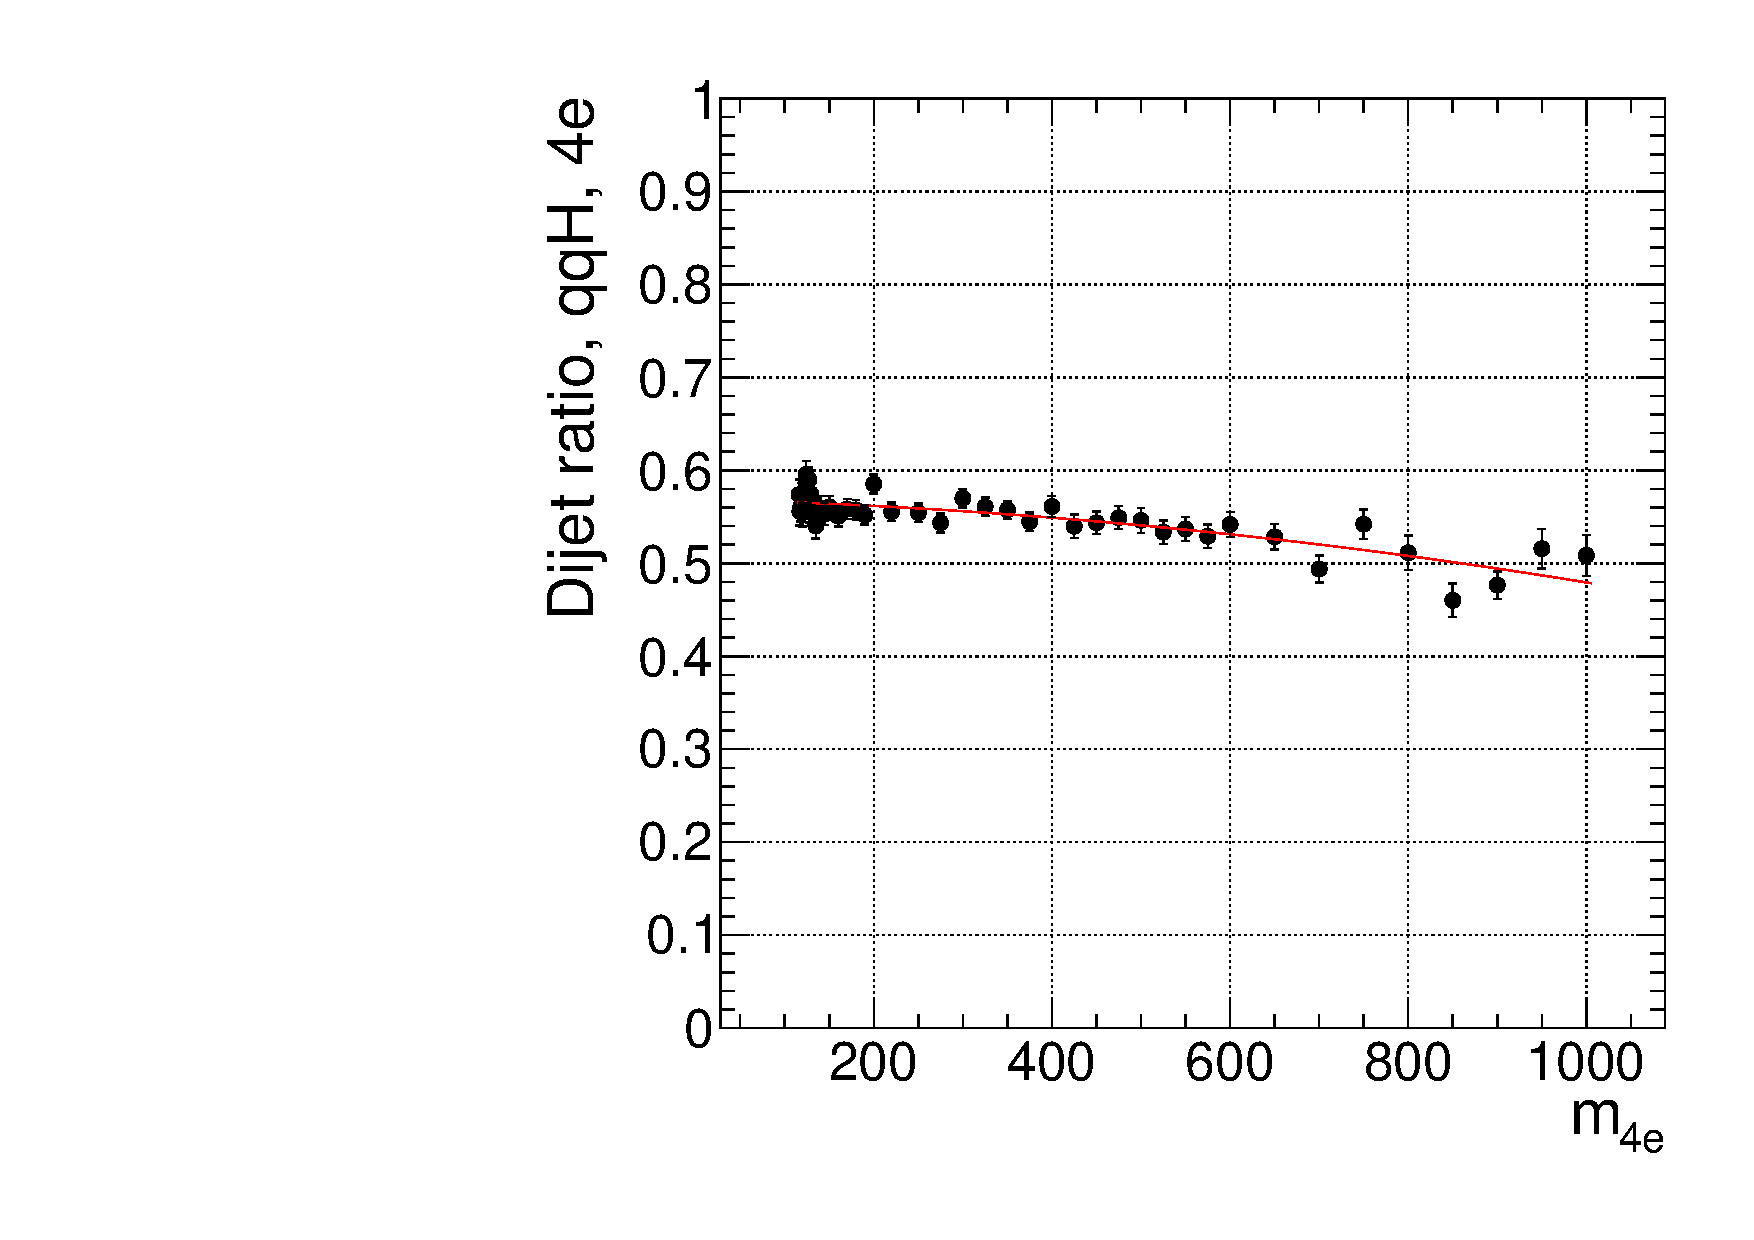
\includegraphics[width=.3\linewidth]{HiggsDiscovery/figures/eff_qqH_4e_ratio.pdf}
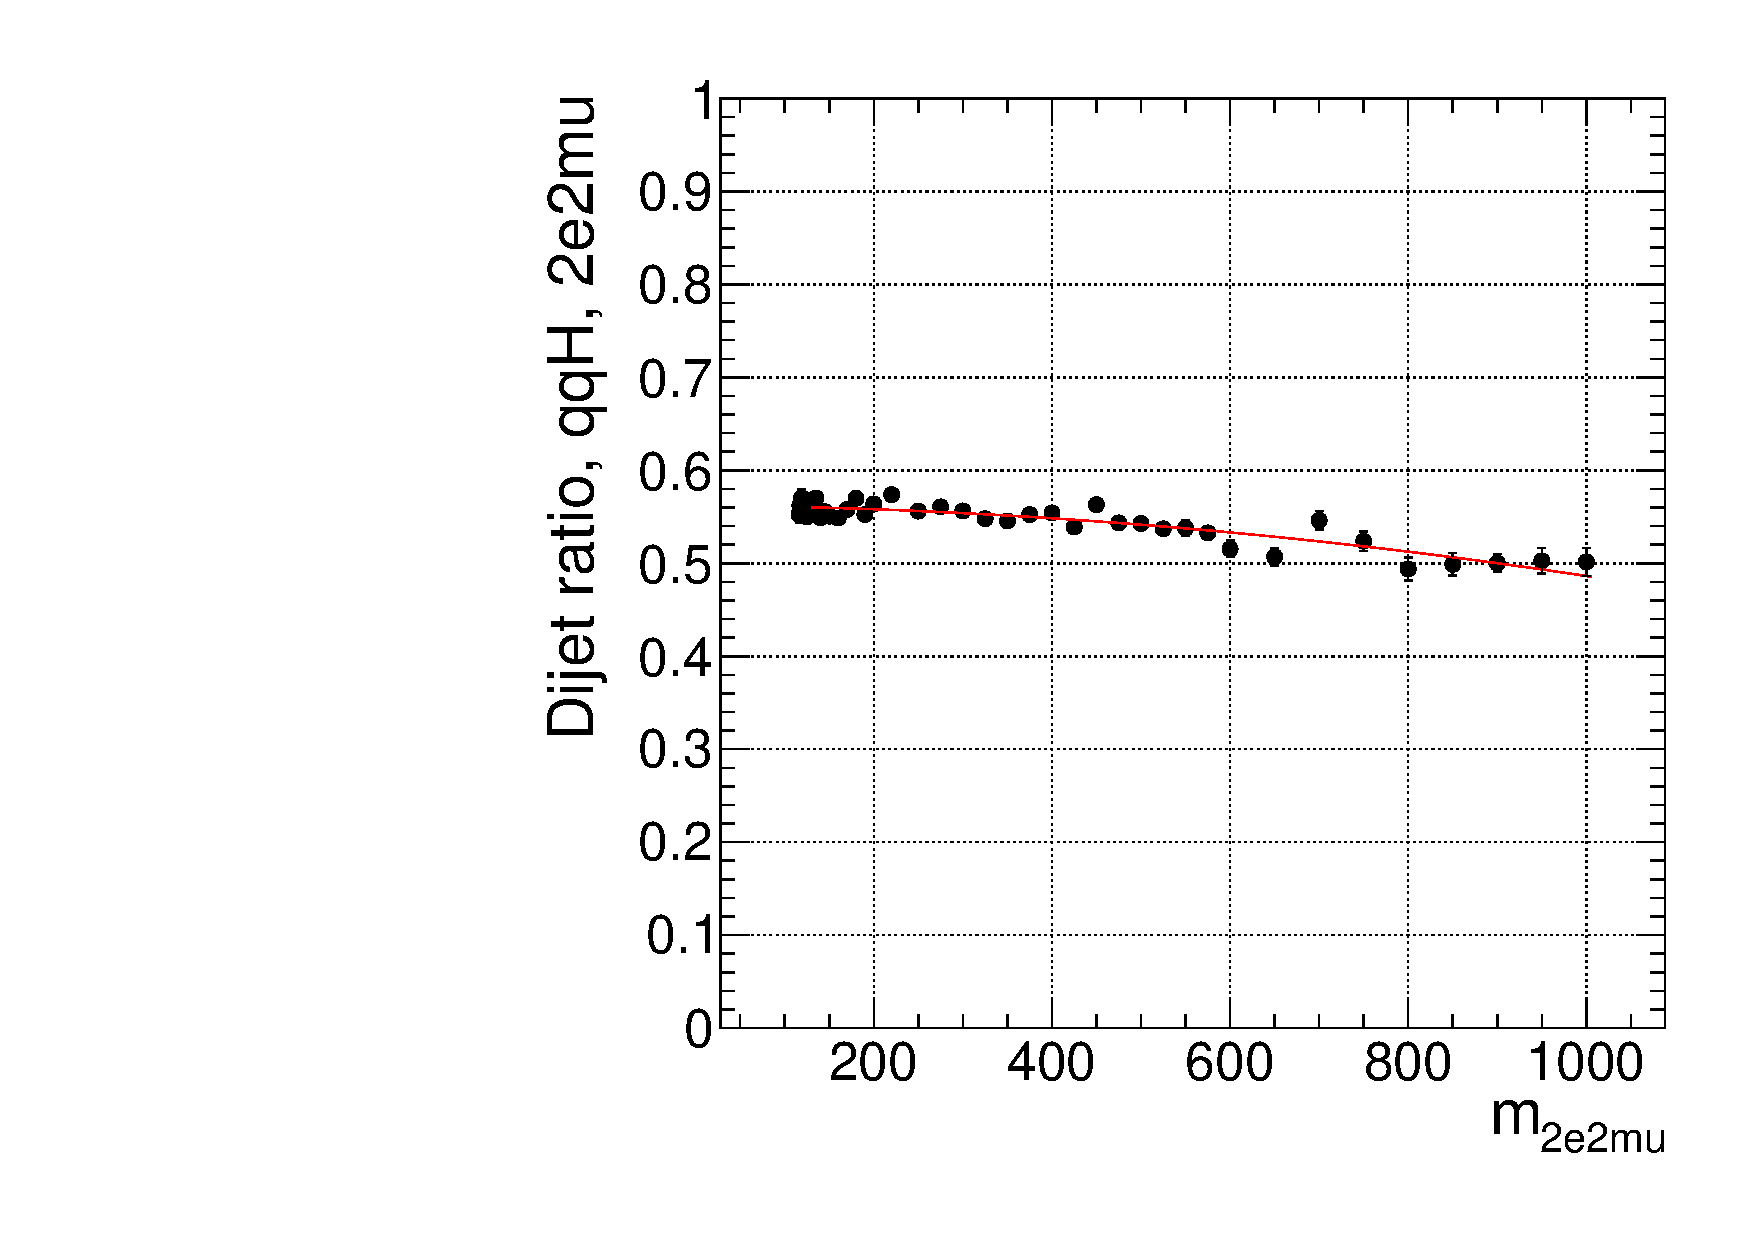
\includegraphics[width=.3\linewidth]{HiggsDiscovery/figures/eff_qqH_2e2mu_ratio.pdf}
\caption[Dijet Ratio of Gluon Fusion and Weak Vector Boson Fusion as Function of $m_H$]{Dijet ratio of ggF (top row) and VBF (bottom row) as functions of $m_H$. Left to right: $4\mu$, $4e$, $2e2\mu$. There should be very correlation between the Higgs final state and the dijet ratio, which is exactly what is seen.}
\label{fig:DijetRatioggHqqH}
\end{center}
\end{figure}

\begin{figure}[htbp]
\begin{center}
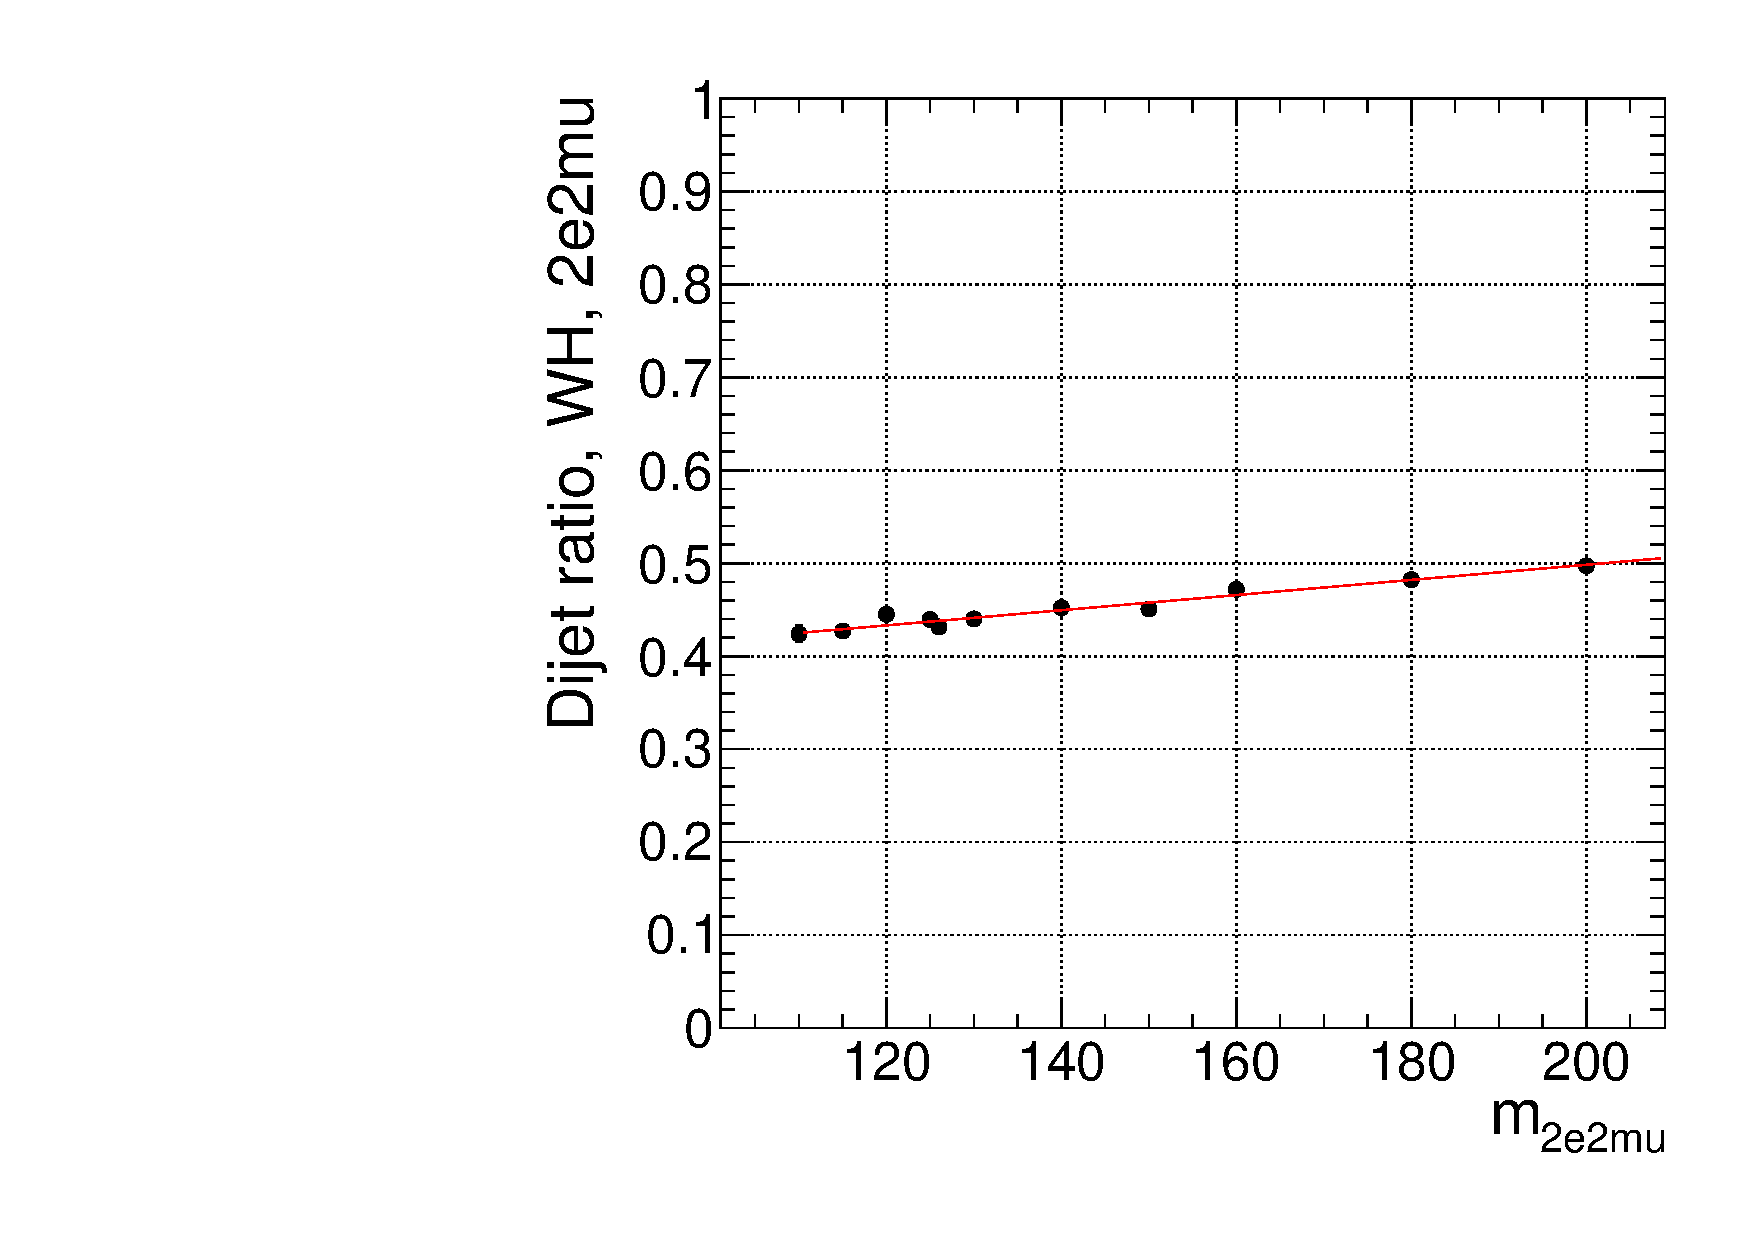
\includegraphics[width=.3\linewidth]{HiggsDiscovery/figures/eff_WH_2e2mu_ratio.pdf}
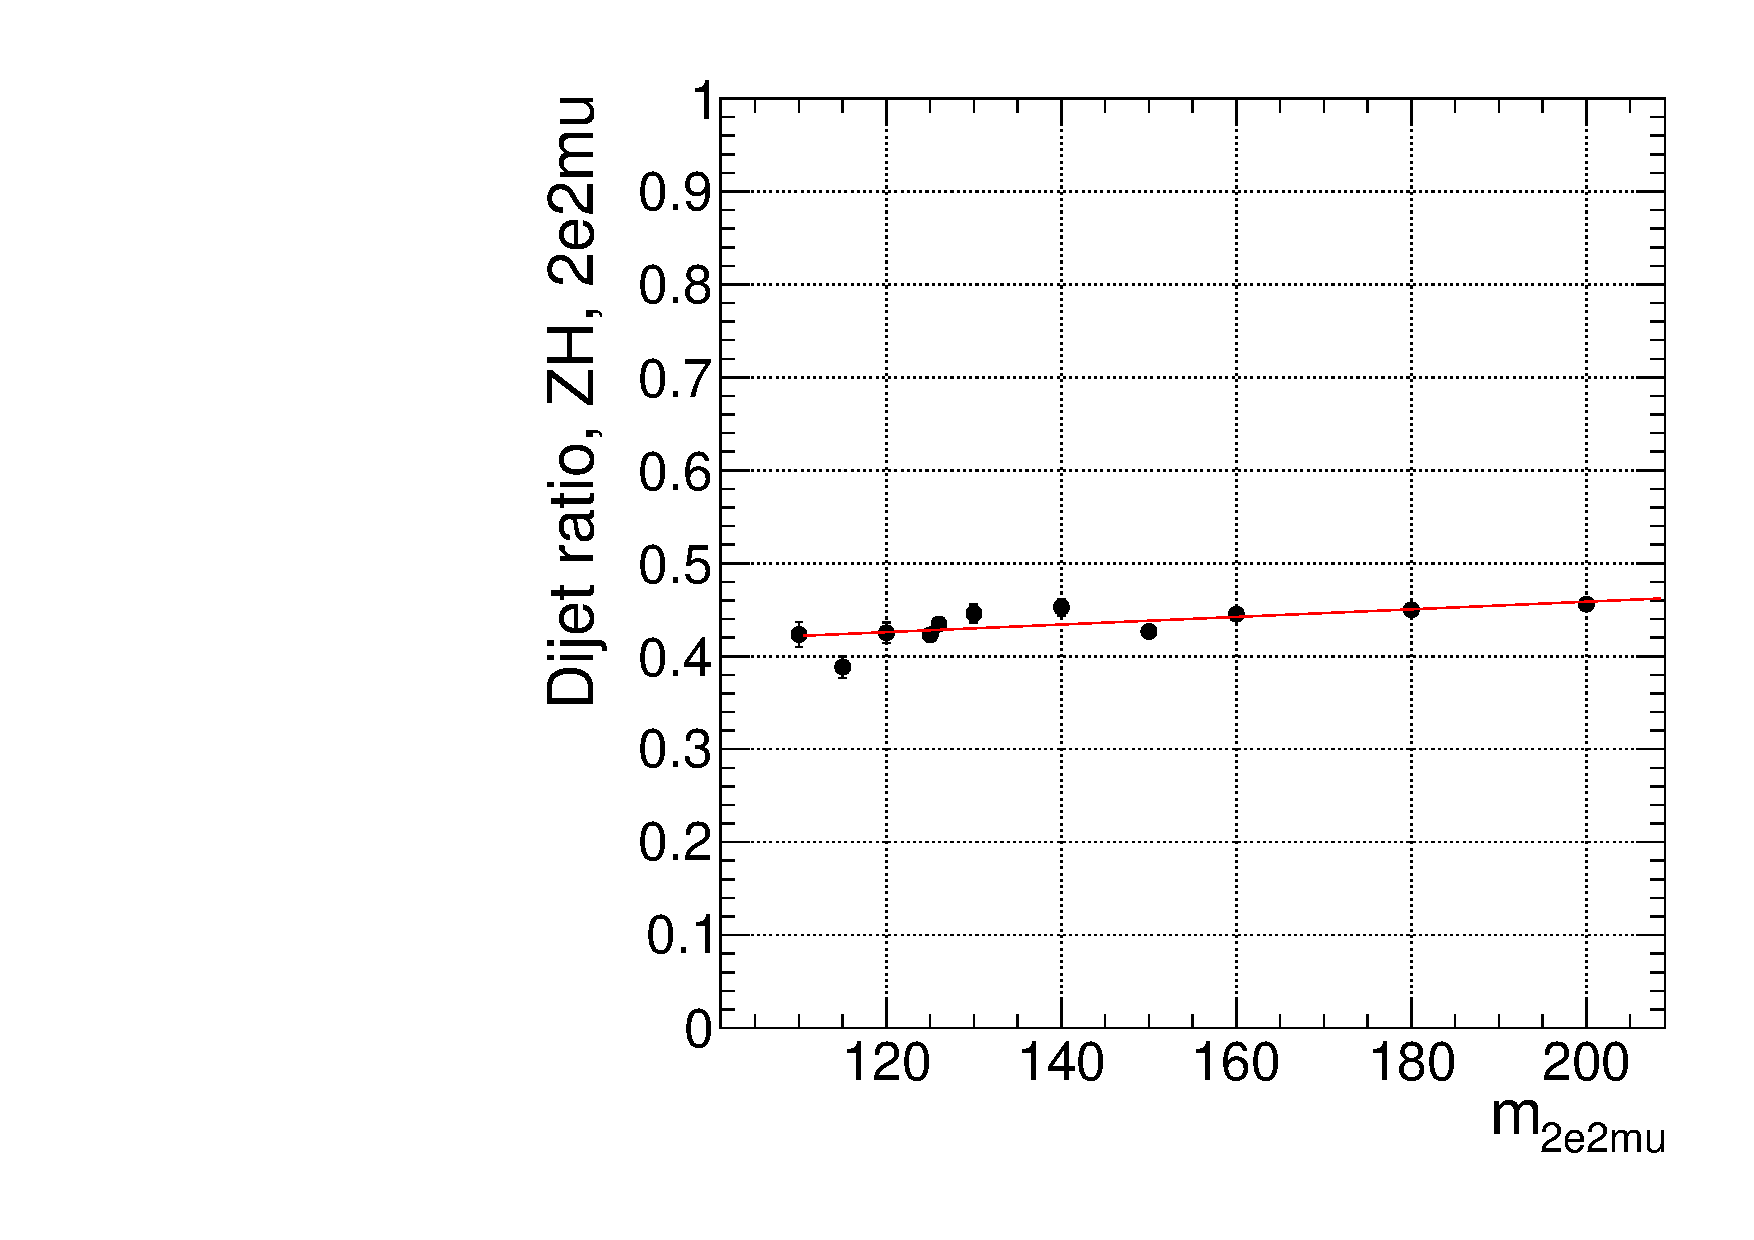
\includegraphics[width=.3\linewidth]{HiggsDiscovery/figures/eff_ZH_2e2mu_ratio.pdf}
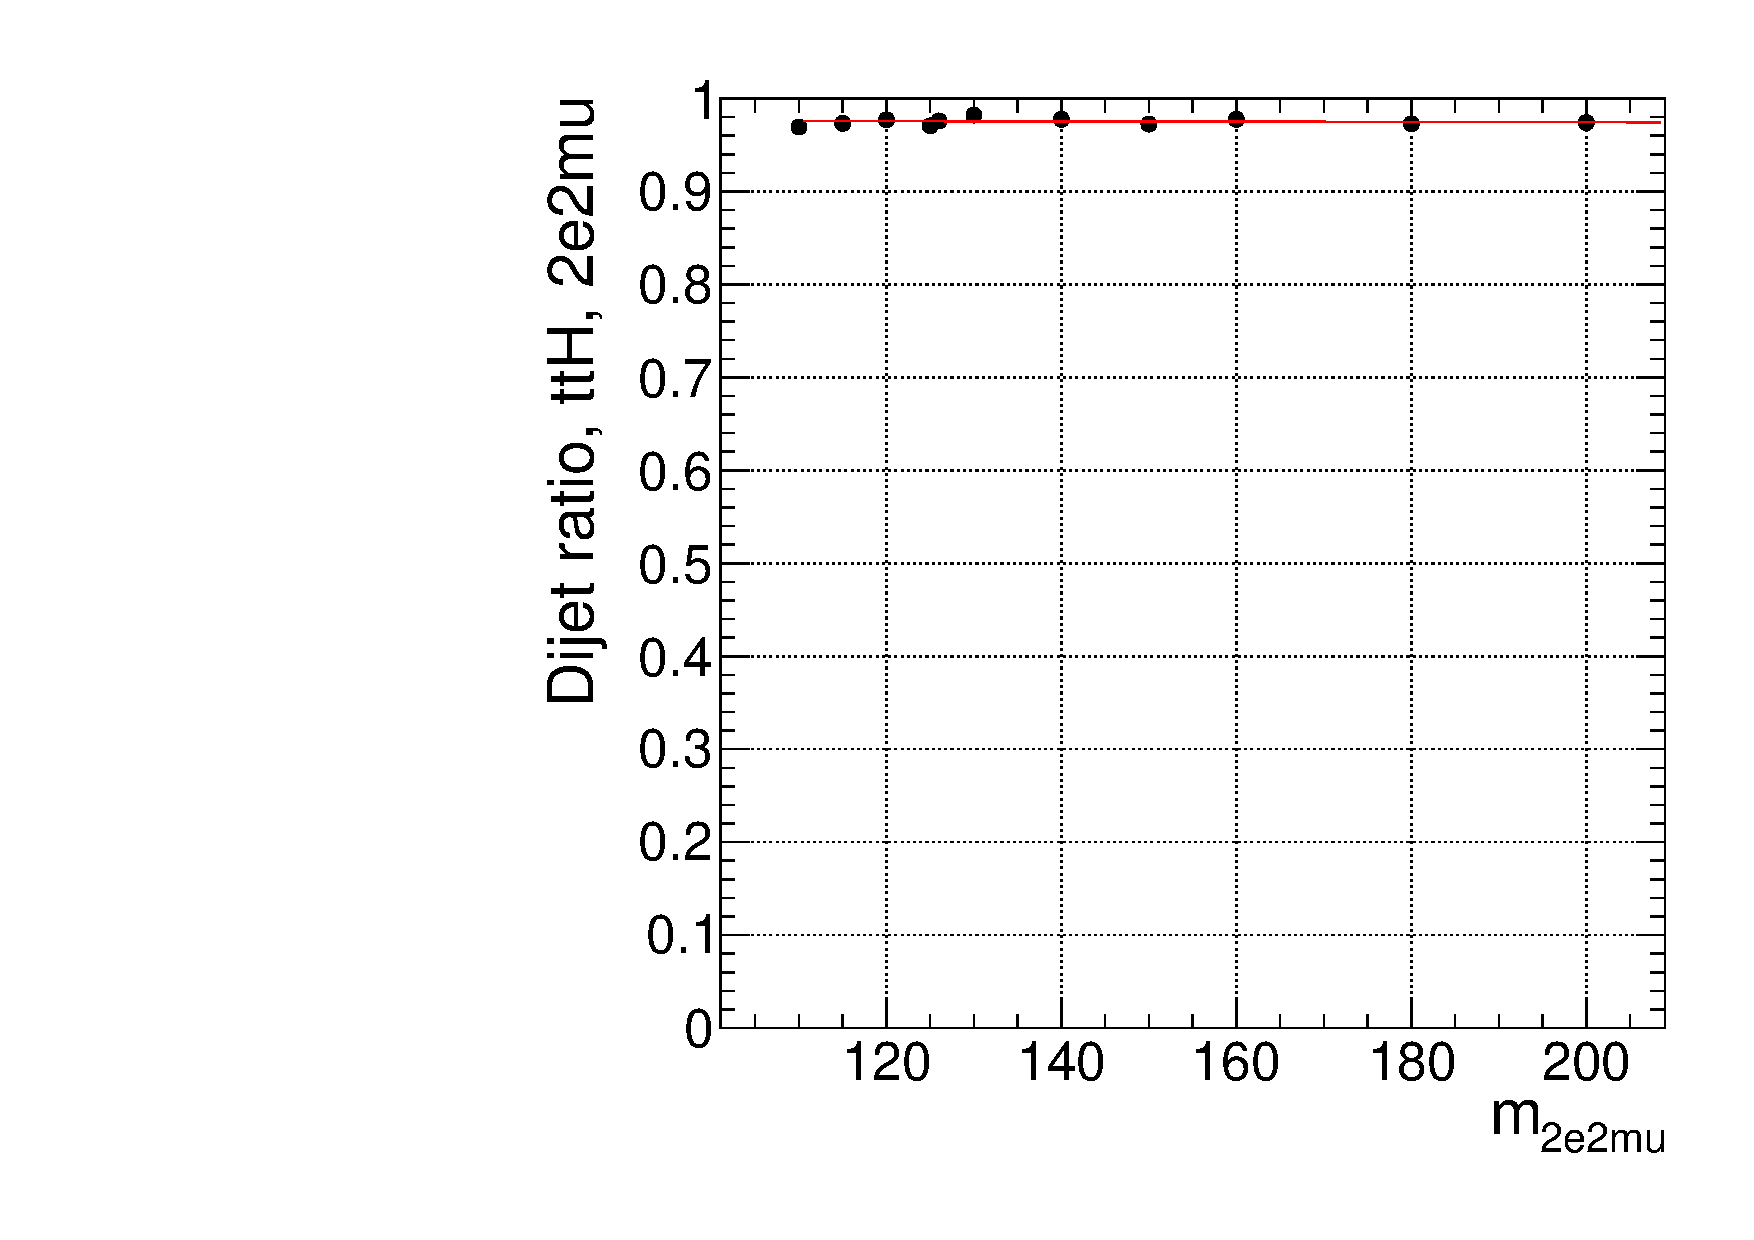
\includegraphics[width=.3\linewidth]{HiggsDiscovery/figures/eff_ttH_2e2mu_ratio.pdf}
\caption[Dijet Ratio of Associated Production as Function of $m_H$]{Dijet ratio of WH (left), ZH (middle), and ttH (right). ttH inherently involves the production of two jets, so the ratio will be nearly 100\%.}
\label{fig:DijetRatioAss}
\end{center}
\end{figure}

Whether an event falls into the dijet or non-dijet category determines what observables are used for the analysis. In the non-dijet category, Higgs events, particularly those generated via other production mechanisms than ggF, will tend to have higher $p_T$ distributions, seen in Fig.~\ref{fig:HiggspT}. To aid in discrimination of production mechanisms, $p_T$ can be used as an observable in the non-dijet category.

For signal, $p_T$ distributions are found via analytic fits of MC simulation, with some reweighting for ggF high mass samples to account for theoretical limitations and to bring the LO $p_T$ distributions of associated Higgs production in agreement with NLO simulation. Shape systematics come from the choice of scales used theoretical predictions, top-mass approximation, and PDF uncertainties for ggF and VBF, while associated production methods have systematics from the reweighting procedure applied. For the irreducible $ZZ$ backgrounds, analytical fits come from MC reweighted to account for differences between data and MC \cite{}, where shape systematics are identical to VBF. $Z+X$, being data driven, is fit with a modified Tsallis function \cite{} where systematics come from uncertainty of the fit. Due to small differences in resolution based on $p_T$, there is a slight dependence of $\mathcal{D}_{\rm{bkg}}^{\rm{kin}}$ on $p_T$ which is accounted for in the shape systematics. Example 2D templates of $(p_T,m_{4l})$ to be used in the analysis are seen in Fig.~\ref{fig:pTTemplates}.

\begin{figure}[htbp]
\begin{center}
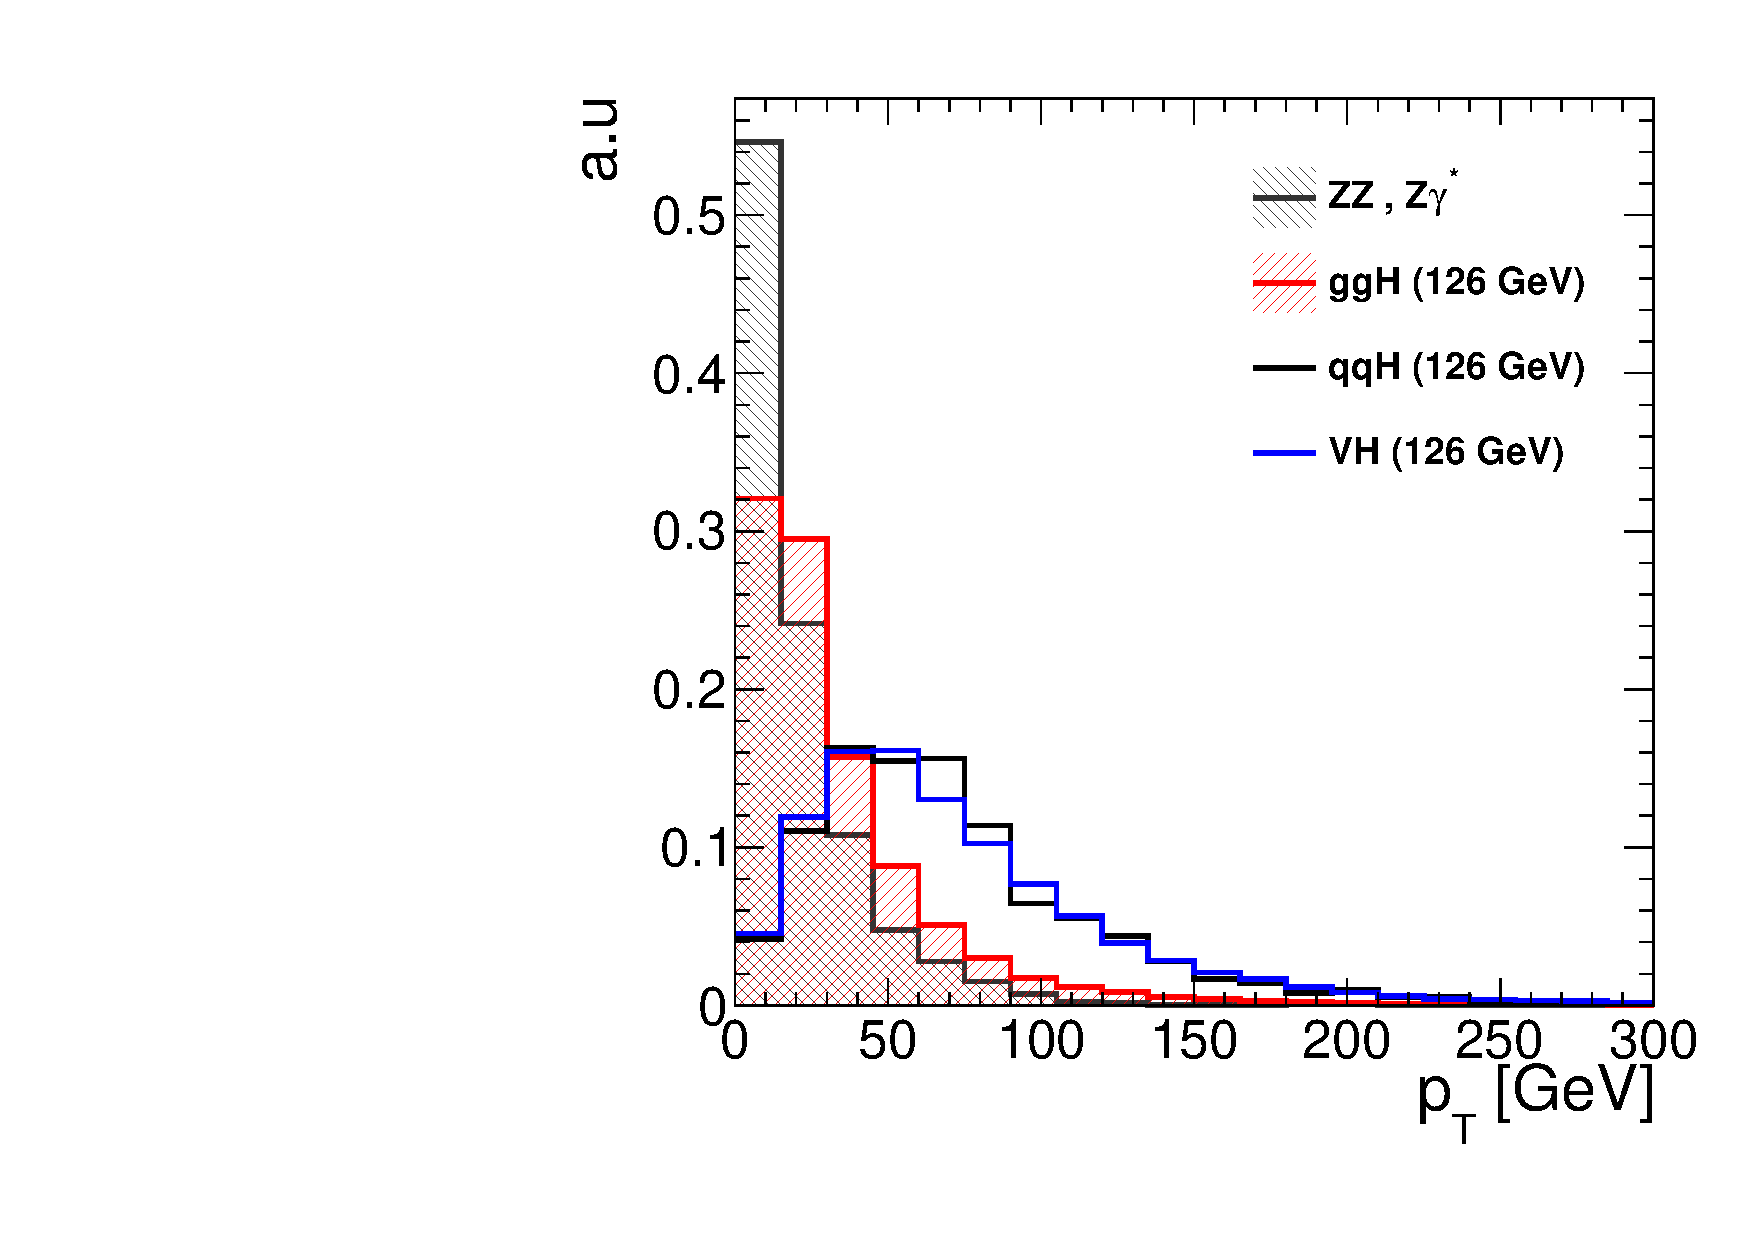
\includegraphics[width=.4\linewidth]{HiggsDiscovery/figures/pt_shape.pdf}
\caption[Transverse Momentum Shapes of Different Higgs Production Mechanisms]{$p_T$ distributions for ggF (hashed red), VBF (black), VH (blue), and the dominant $q\bar{q}$ background (hashed black). Subdominant production mechanisms have harder $p_T$ spectra than either ggF or the $q\bar{q}$ background, so it can used to discriminate production mechanisms.}
\label{fig:HiggspT}
\end{center}
\end{figure}

\begin{figure}[htbp]
\begin{center}
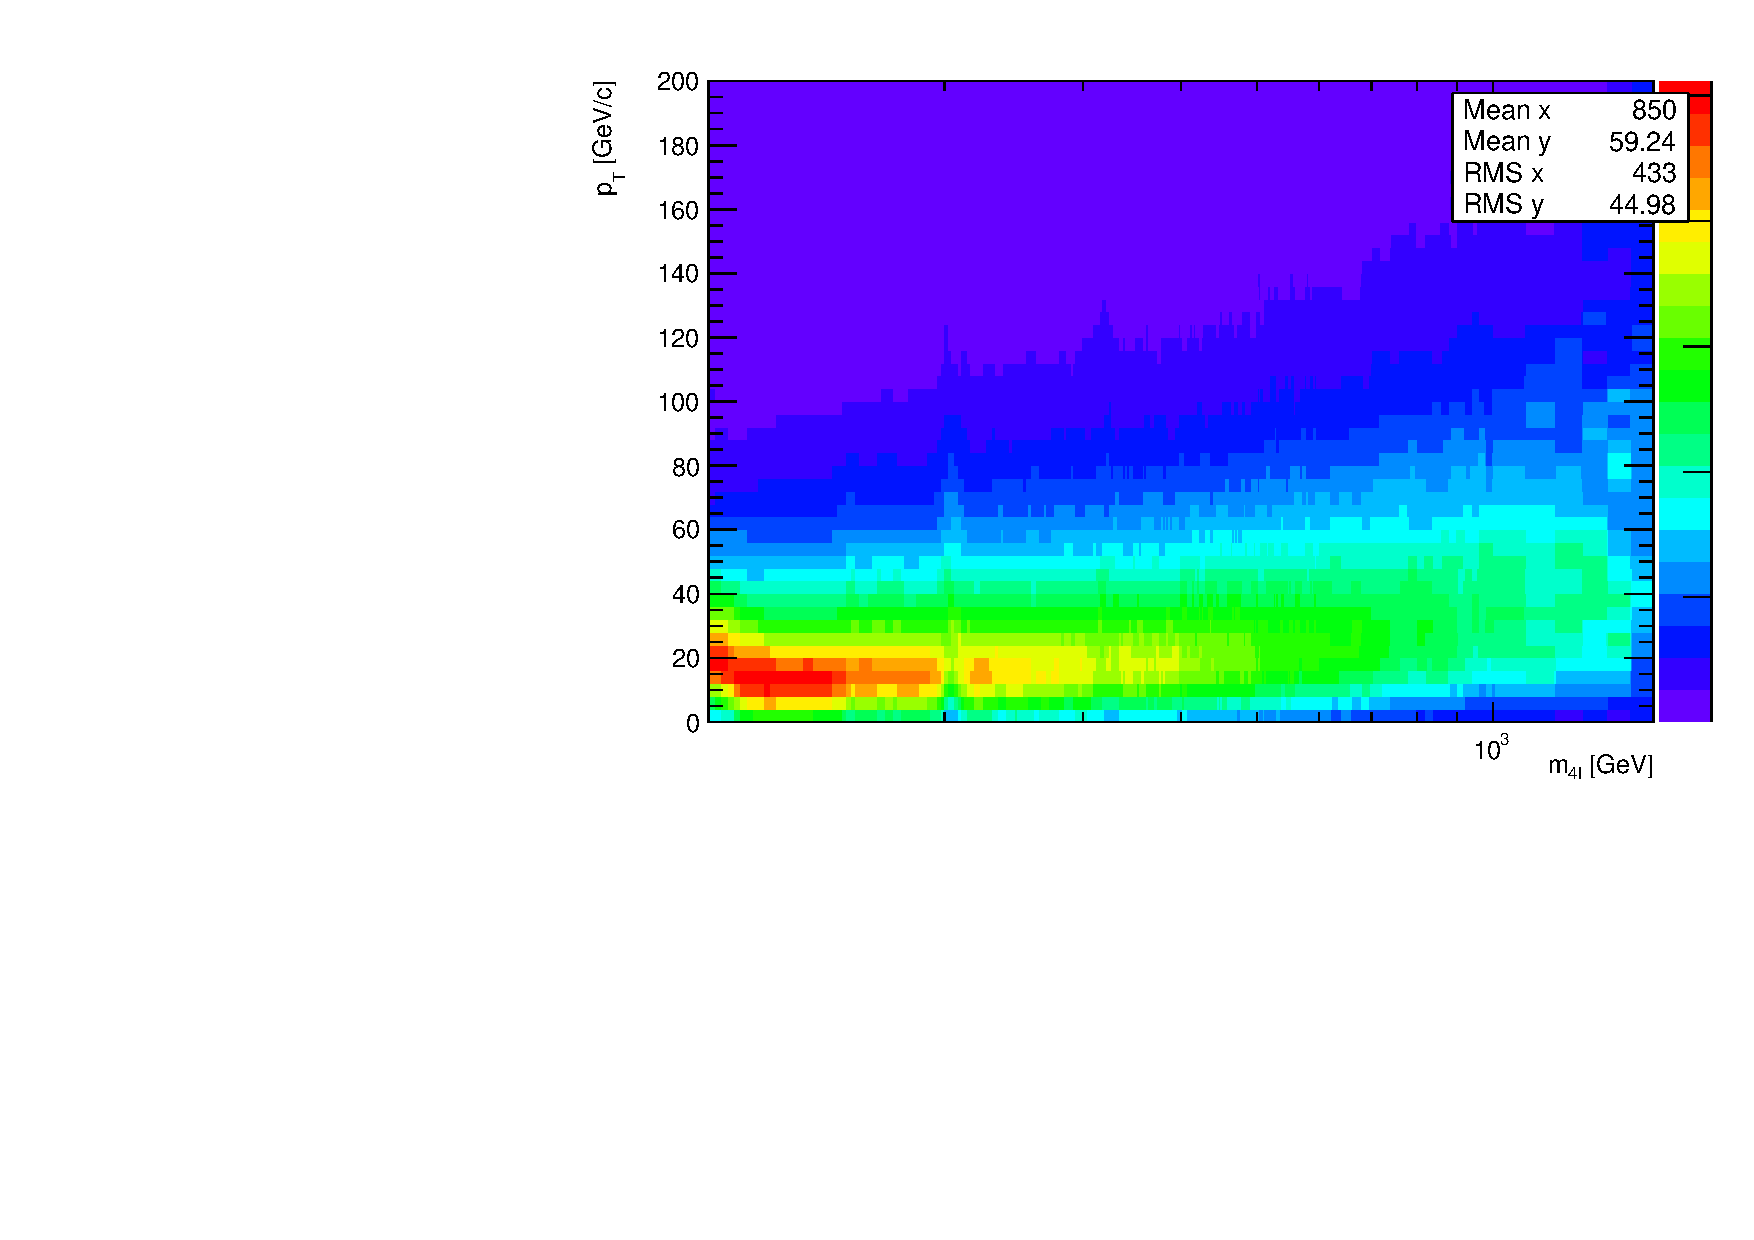
\includegraphics[width=.3\linewidth]{HiggsDiscovery/figures/ptrestricted_ggDefaultTemplate_8TeV.pdf}
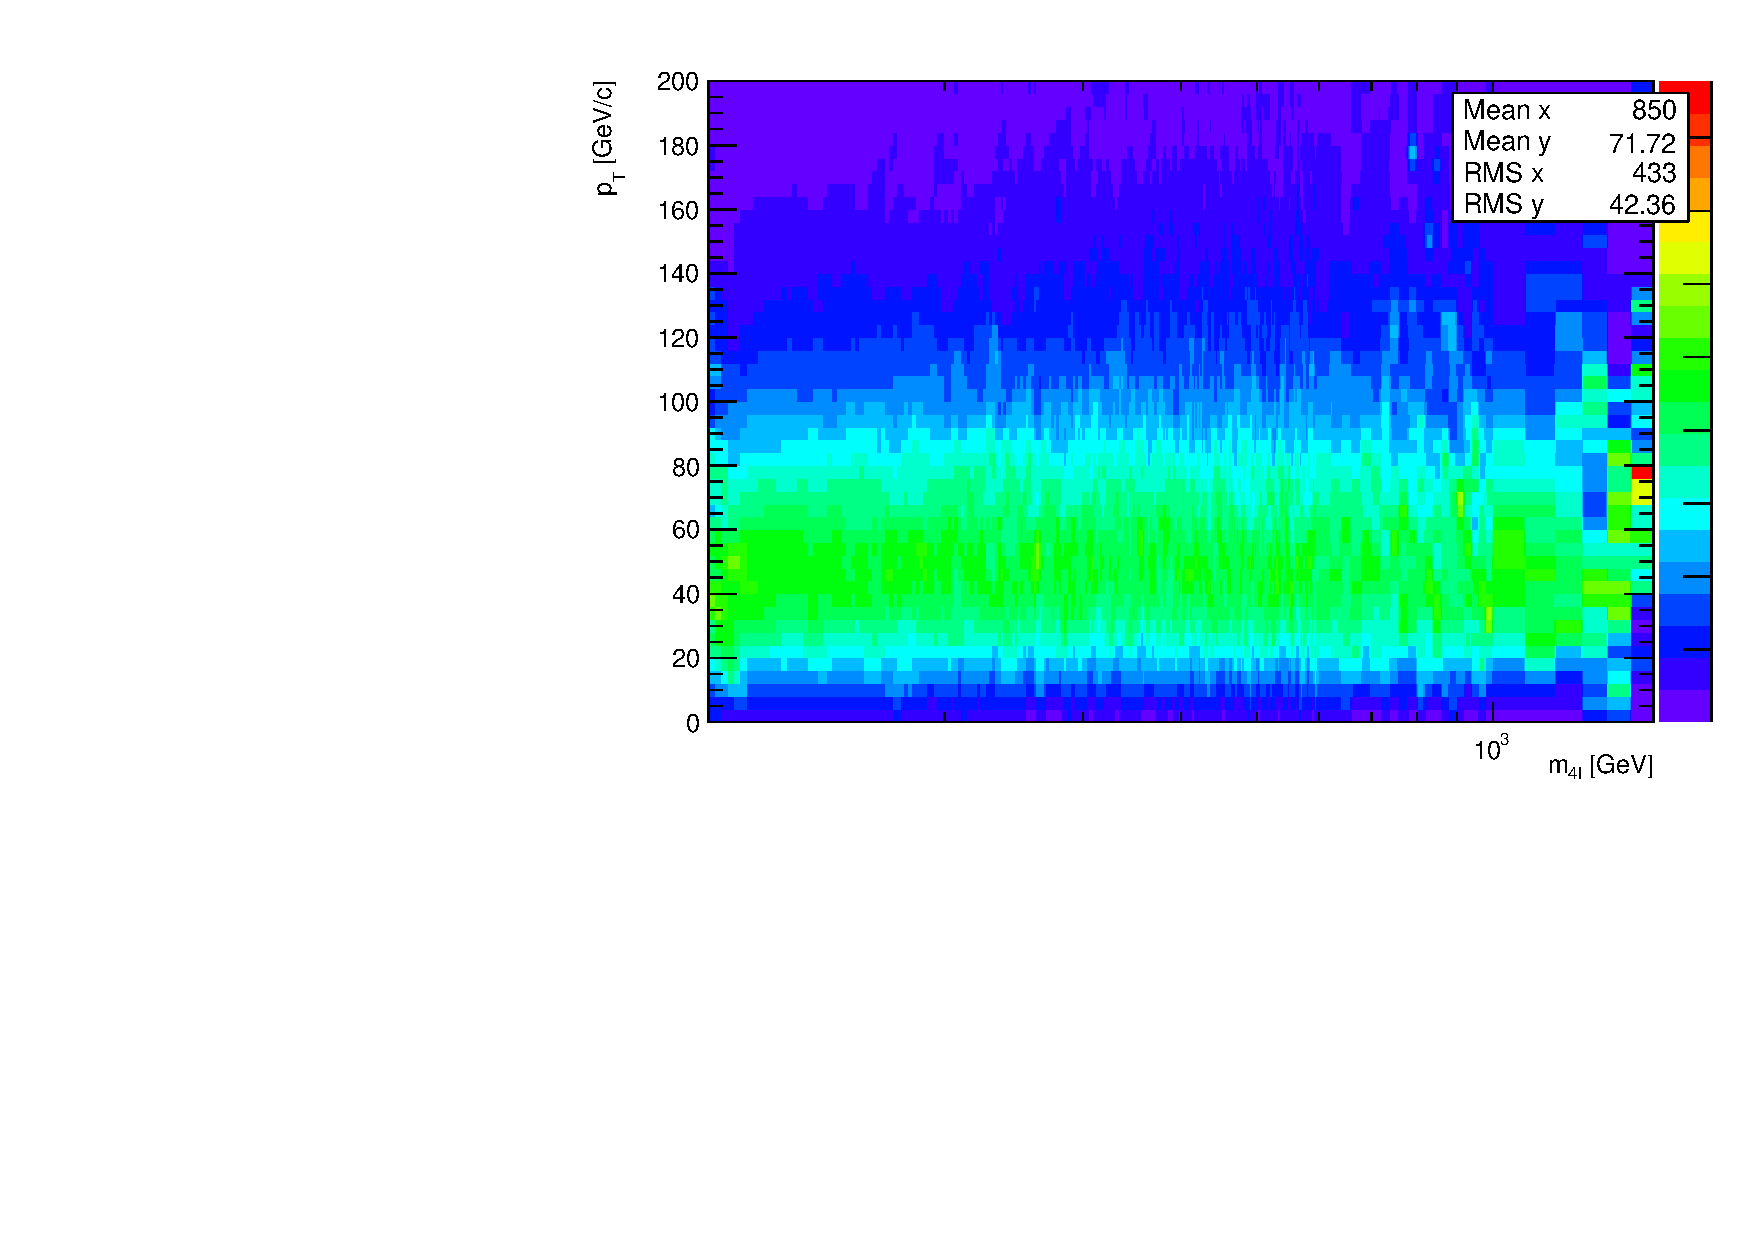
\includegraphics[width=.3\linewidth]{HiggsDiscovery/figures/ptrestricted_vbfDefaultTemplate_8TeV.pdf}
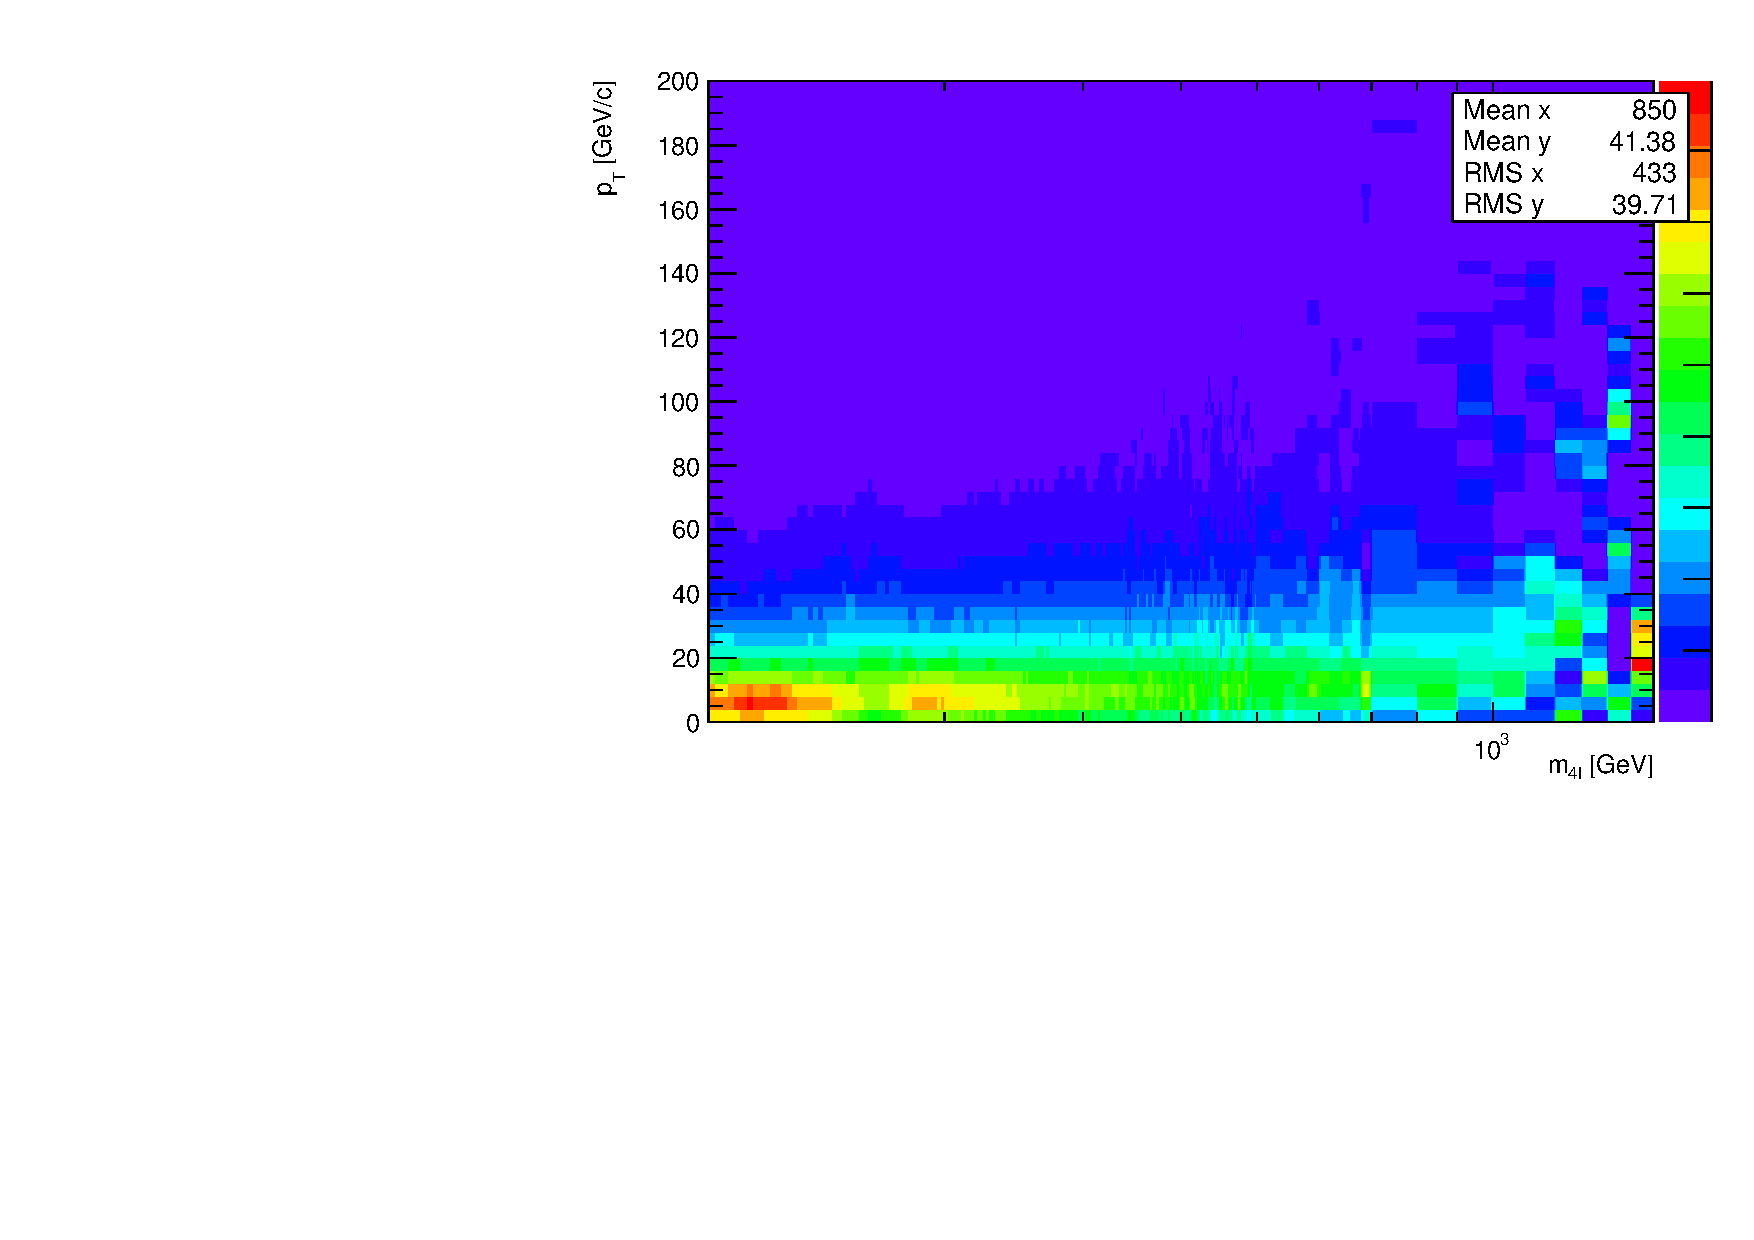
\includegraphics[width=.3\linewidth]{HiggsDiscovery/figures/ptrestricted_zzDefaultTemplate_8TeV.pdf}
\caption[Templates of Transverse Momentum for $4l$ Signals and Background]{Samples of $p_T$ v $m_{4l}$ templates for 8 $\rm{TeV}$ ggF (left), VBF (middle), and $q\bar{q}\rightarrow ZZ$ (right) used in the analysis. Other templates were made and used for WH, ZH, and $gg\rightarrow ZZ$.}
\label{fig:pTTemplates}
\end{center}
\end{figure}

For any dijet event, the combined kinematics of the jets can be examined. In the initial discovery and property measurements of the Higgs, a matrix element technique was not yet developed so a linear discriminant \cite{} was built to optimize separation between VBF and ggF production mechanisms. Using the leading and subleading jets, $m_{JJ}$ and $\Delta\eta_{JJ}$ form the two variables for the discriminant. The optimal combination, trained on {\tt POWHEG} ggF and VBF samples, is
\begin{equation} \label{eq:HiggsFisher}
D_{jet} = 0.18\Delta\eta_{JJ} + 1.92\times10^{-4}m_{JJ}
\end{equation}
This formulation is then implemented for different MC samples (or control region for $Z+X$) to form the 2D $(m_{4l},D_{jet})$ templates. Shape systematics are applied for each template, coming from the largest deviations in available alternative shapes for the respective sample: choice of MC generator, choice of hadronization tuning, or jet energy scale corrections. Sample templates are seen in Fig.~\ref{fig:FisherTemplates}.

\begin{figure}[htbp]
\begin{center}
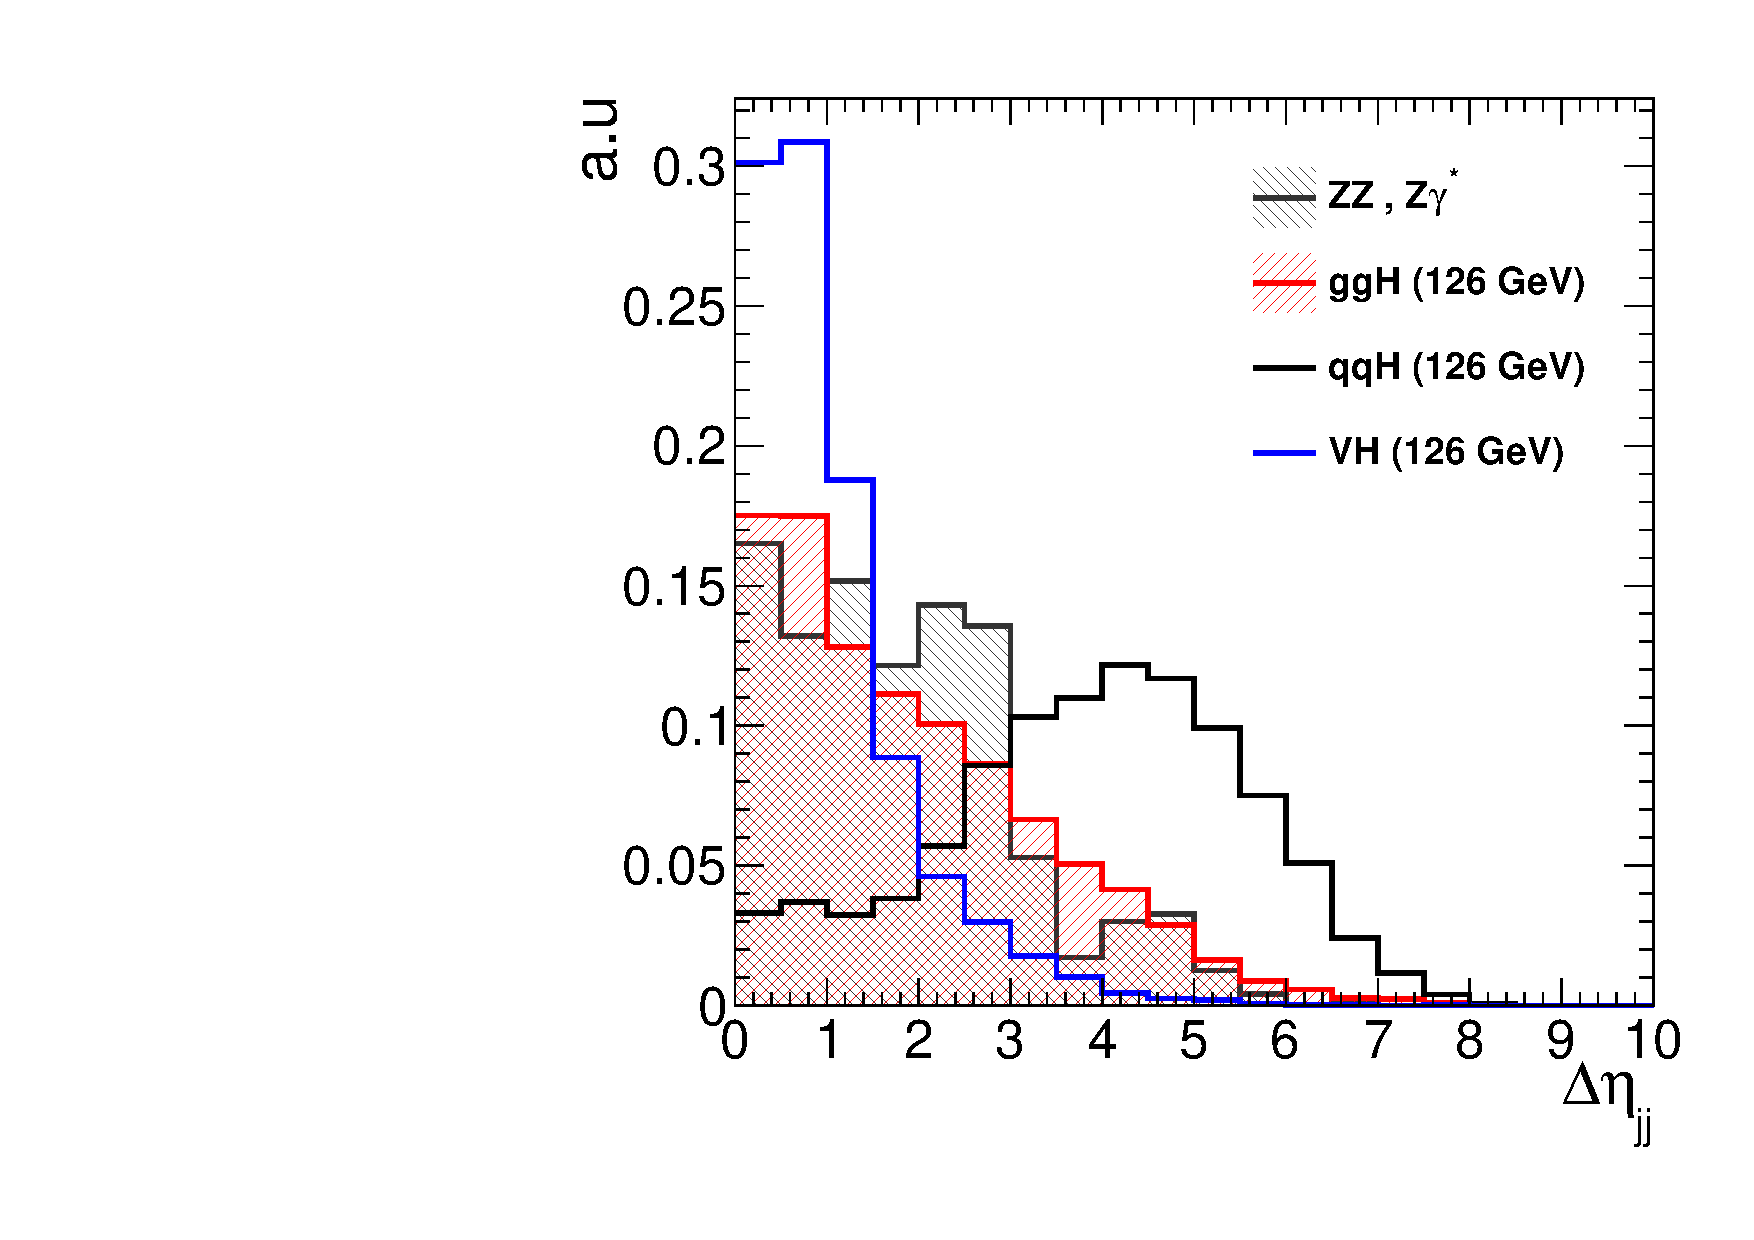
\includegraphics[width=.3\linewidth]{HiggsDiscovery/figures/deta_shape.pdf}
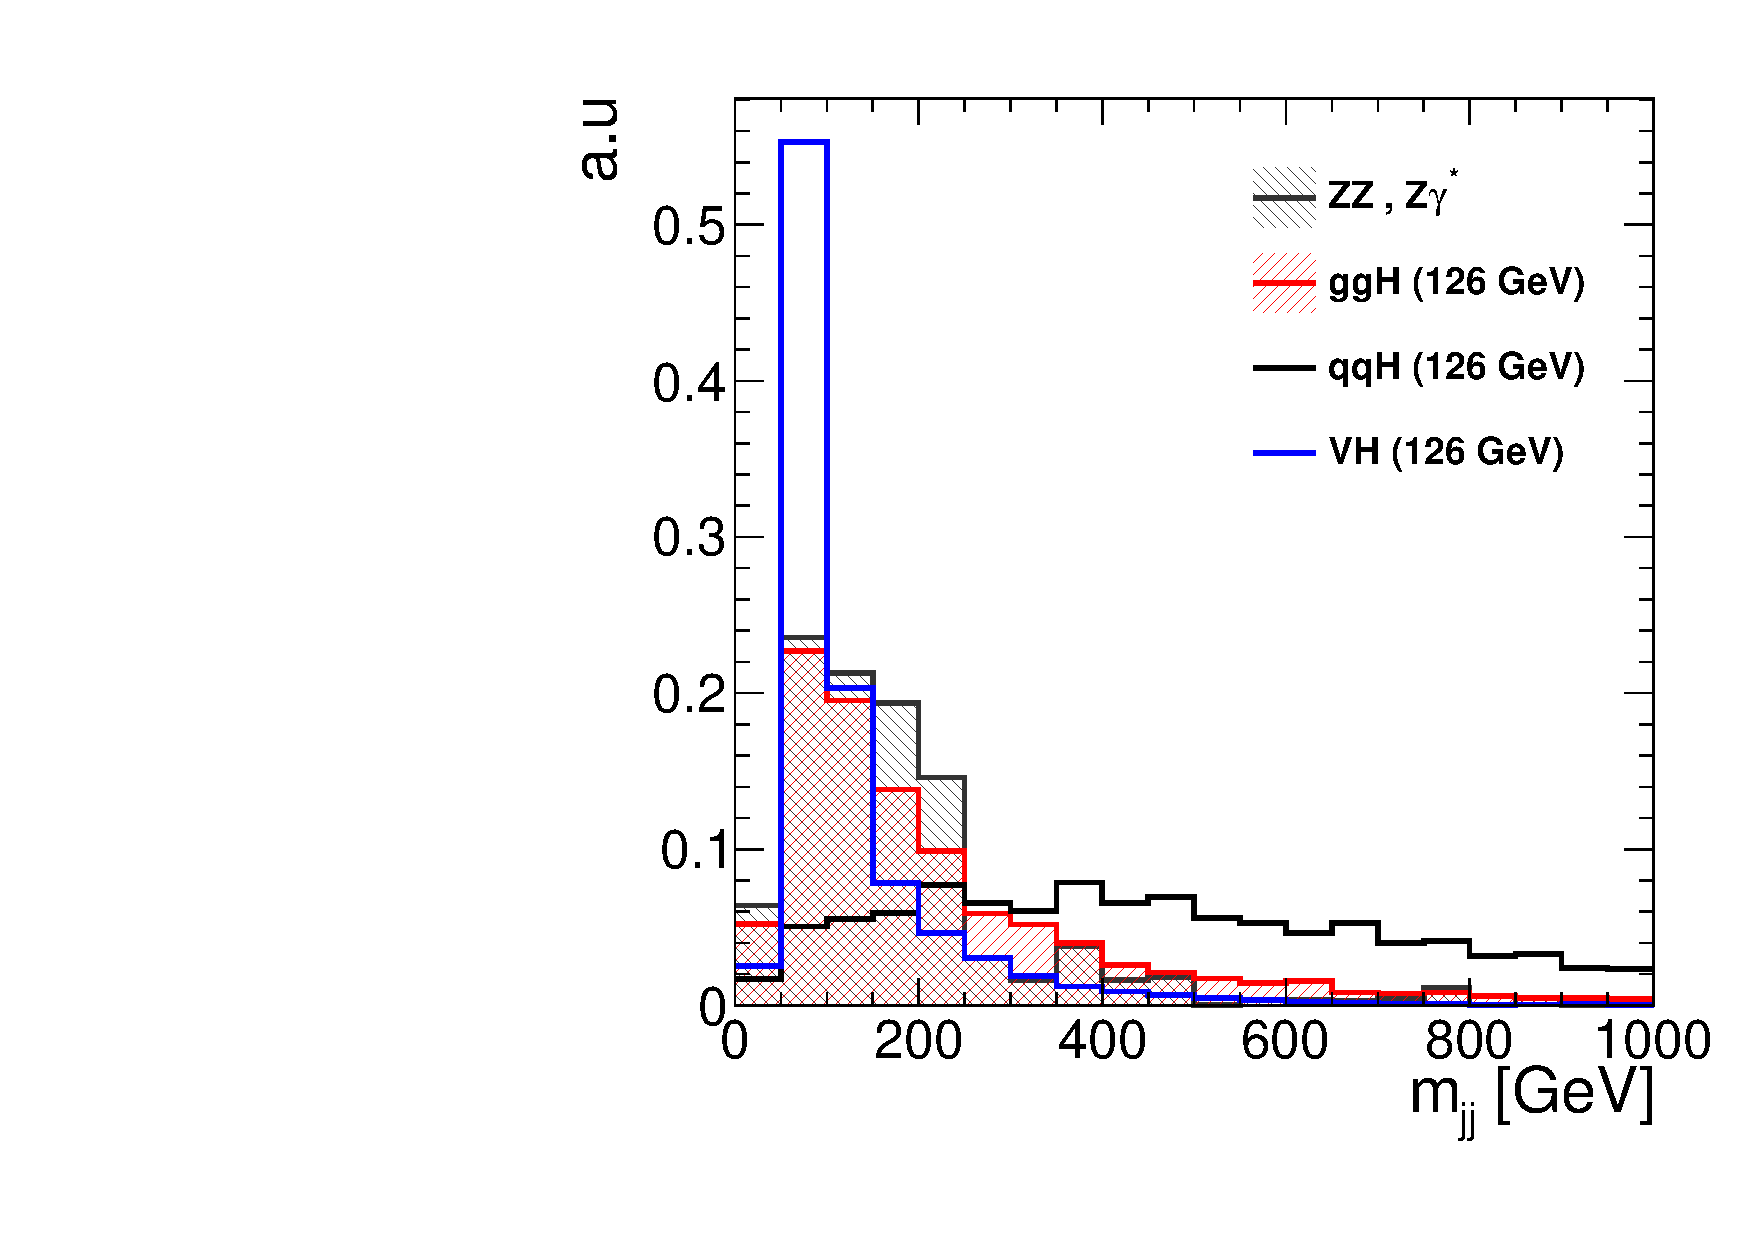
\includegraphics[width=.3\linewidth]{HiggsDiscovery/figures/mjj_shape.pdf}
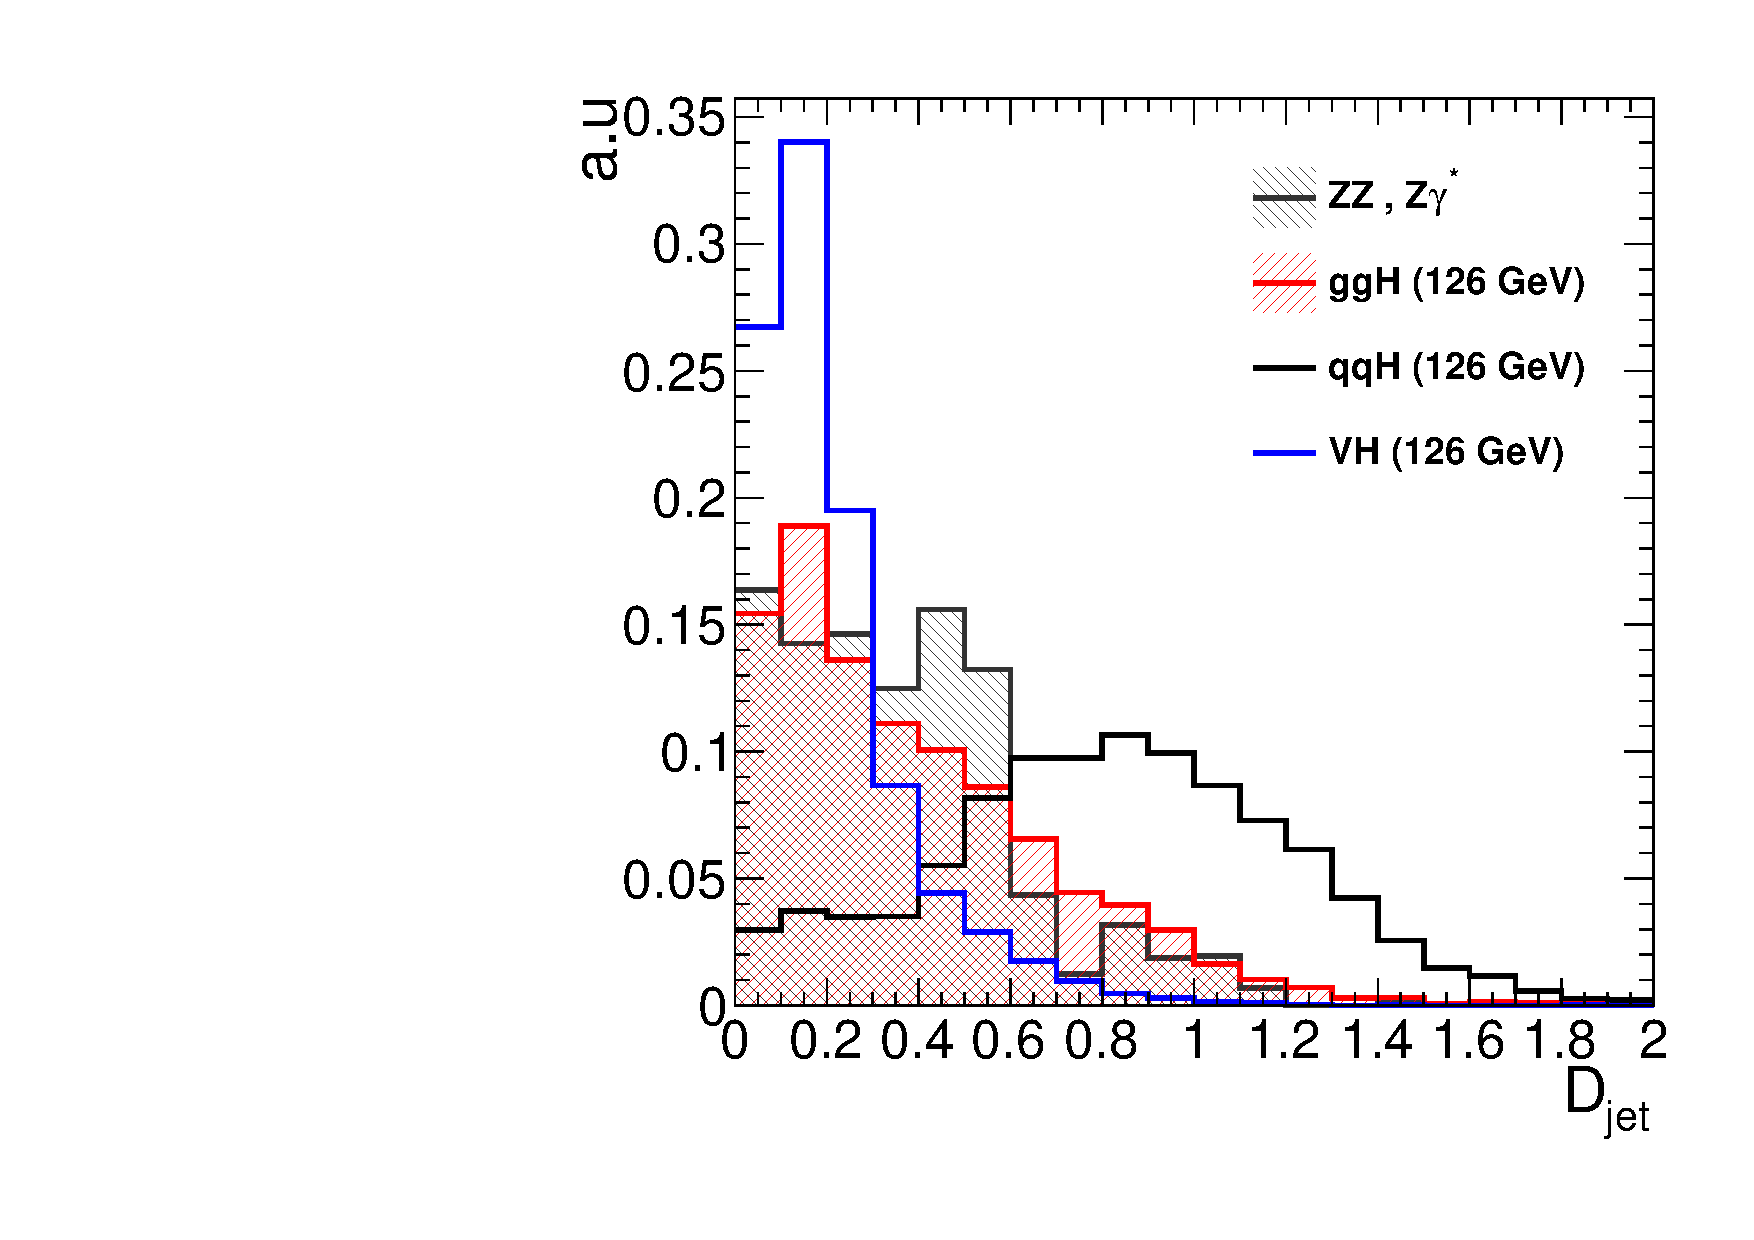
\includegraphics[width=.3\linewidth]{HiggsDiscovery/figures/djet_shape.pdf} \\
\caption[Jet Kinematic Shapes of Different Higgs Production Mechanisms]{$\Delta\eta_{JJ}$ (left) and $m_{JJ}$ (middle) distributions for ggF (hashed red), VBF (black), VH (blue), and the dominant $q\bar{q}$ background (hashed black). These are used as input for the linear discriminant (right, defined in Eq.~\ref{eq:HiggsFisher}).}
\label{fig:HiggsFisher}
\end{center}
\end{figure}

\begin{figure}[htbp]
\begin{center}
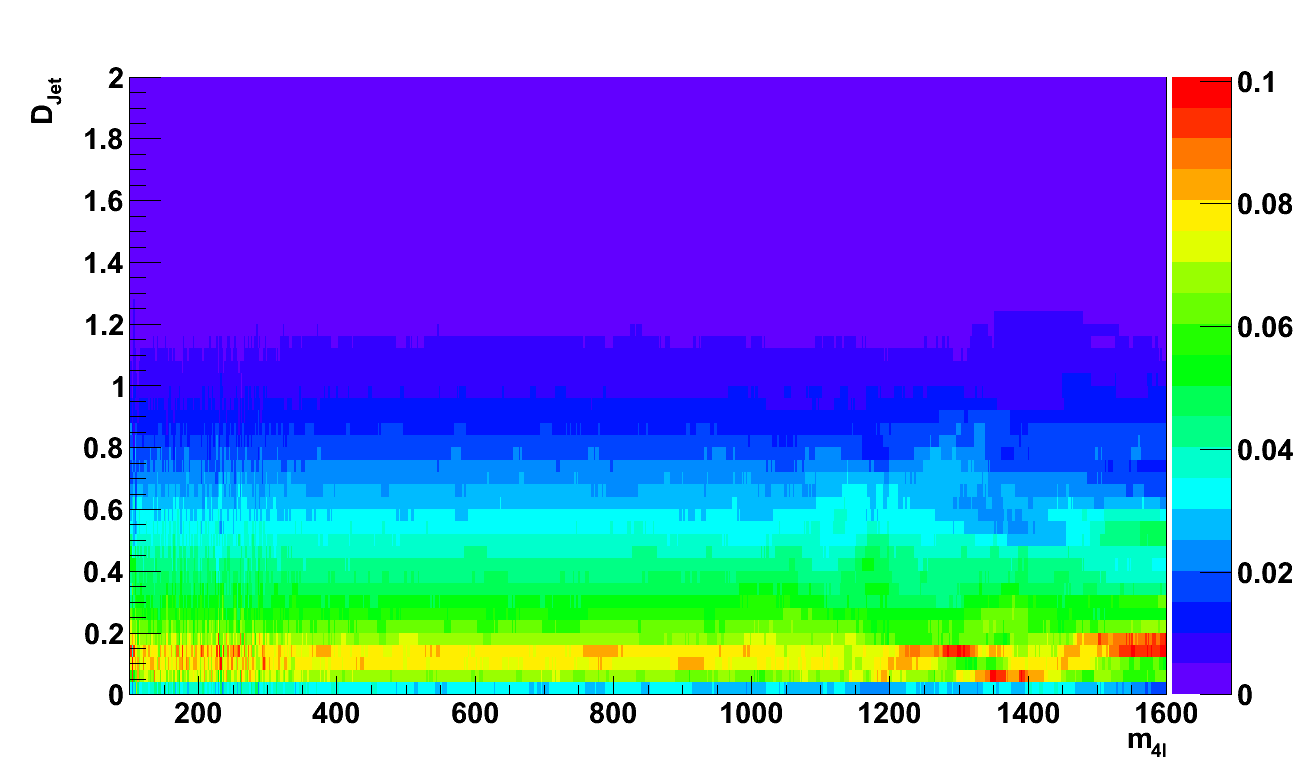
\includegraphics[width=.3\linewidth]{HiggsDiscovery/figures/ggH_Fisher_2D.png}
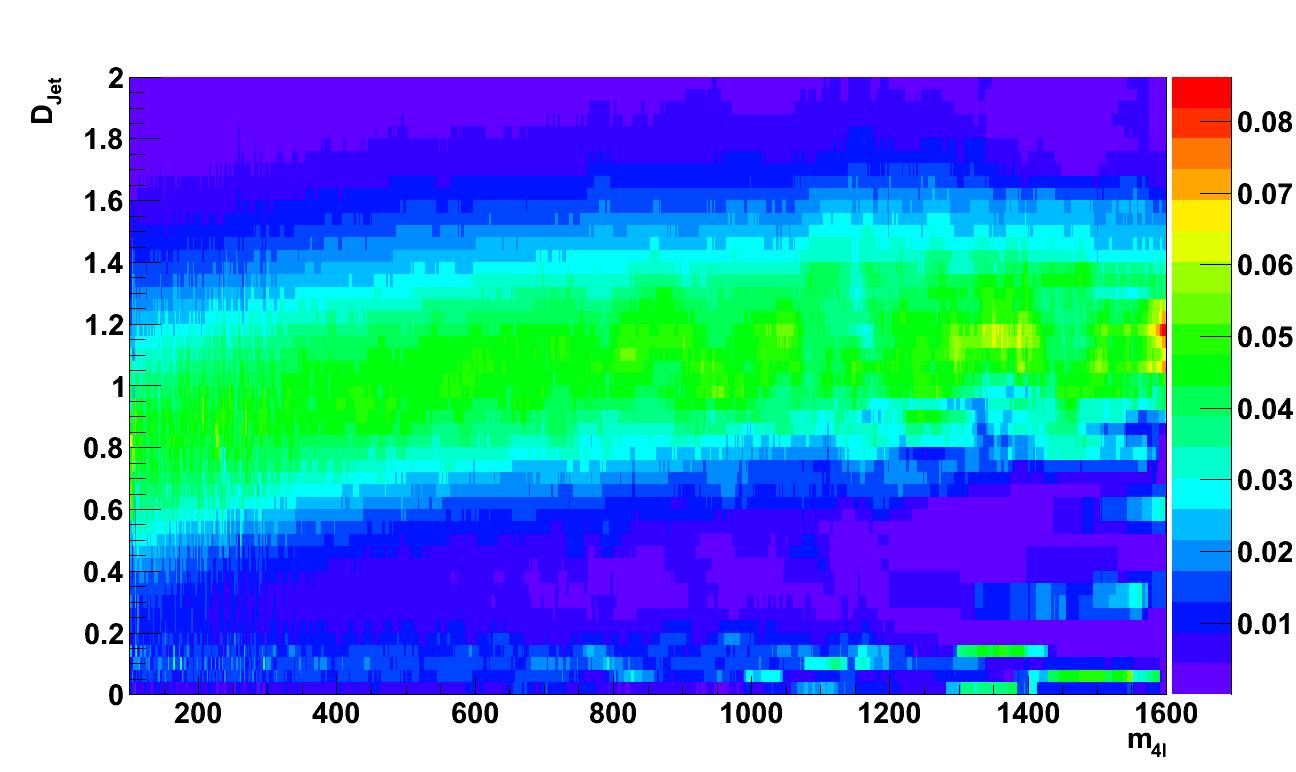
\includegraphics[width=.3\linewidth]{HiggsDiscovery/figures/qqH_Fisher_2D.png}
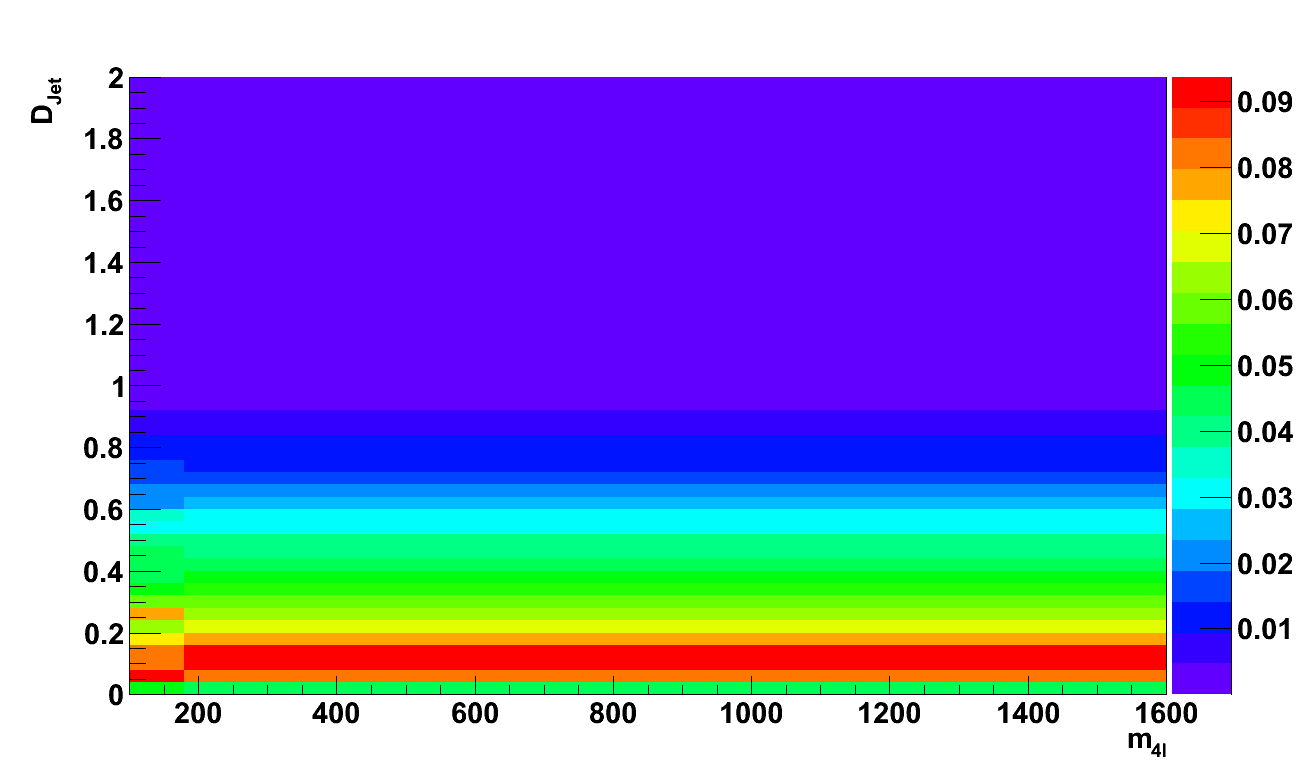
\includegraphics[width=.3\linewidth]{HiggsDiscovery/figures/qqZZ_Fisher_2D.png} \\
\caption[Templates of $D_jet$ for Signals and Background]{Samples of $D_{jet}$ v $m_{4l}$ templates for ggF (left), VBF (middle), and $q\bar{q}\rightarrow ZZ$ (right) used in the analysis. Other templates were made and used for WH, ZH, $\rm{t\bar{t}H}$, $gg\rightarrow ZZ$, and $Z+X$. As there are no appreciable differences between decay mode (see Figs.~\ref{fig:DijetRatioggHqqH} and \ref{fig:DijetRatioAss}) nor beam energy, one 2D template is used for each production method or background.}
\label{fig:FisherTemplates}
\end{center}
\end{figure}

On top of any normalization or shape systematics applied, to account for the uncertainty of jet categorization, we used the suggestions of the JetMET group \cite{}. For ggF, a 15\% yield uncertainty is used for the non-dijet category and 30-50\% for the dijet category. Given that VBF inherently has two hard jets attached, the uncertainties used are lower: 10\% for the 0 jet category and 5\% for 1 or 2 jet categories.

\subsection{Systematics}
\label{sec:ZZ4lSystematics}

Broadly speaking, the systematics applied are split into two types: normalization uncertainties and shape uncertainties. Normalization uncertainties imply that there is an uncertainty on the overall number of events that will appear (e.g. for a particular decay mode, background). Shape uncertainties mean that there is uncertainty on how those events will appear, independent of the number (e.g. kinematics of the Higgs production, mass shape of the background). While shape systematics were discussed in earlier section with their respective shapes, Table~\ref{tbl:HZZ4lNormSyst} contains all common normalization systematics applied in this analysis for the $m_H = 126$ $\rm{GeV}$ mass point.

\begin{table}[htbp]
  \begin{center}
    \begin{tabular}{|lccccccc|}
      \hline
      Source         & \multicolumn{4}{c}{Signal ($m_H = 126$ $\rm{GeV}$)}  &  \multicolumn{3}{c|}{Backgrounds} \\
      \hline
      & ggF       & VBF     &  $VH$   &  $t\bar{t}H$ &  $q\bar{q}\rightarrow ZZ$  &  $gg\rightarrow ZZ$  & $Z+X$ \\
      \hline
      $\alpha_S$ + PDF ($gg$)           & 7.2\%         &  \NA      &   \NA                   &  7.8\%       &  \NA                     &  7.2\%            & \NA   \\
      $\alpha_S$ + PDF ($q\bar{q}$)    & \NA             &  2.7\%  &   3.5\%               &  \NA           &  3.4\%                 &  \NA                & \NA   \\
      Missing higher orders           & 7.5\%         &  0.2\%  &  0.4\%, 1.6\%         & 6.6\%        &  2.9\%                 &  24\%             & \NA   \\
      Signal acceptance               & \multicolumn{4}{c}{ 2\% }                                      &  \NA                     & \NA                 & \NA   \\
      BR($H\rightarrow ZZ$)              & \multicolumn{4}{c}{ 2\% }                                      &  \NA                     & \NA                 & \NA   \\
      Luminosity                      & \multicolumn{6}{c}{ 2.6\% }                                                                                 & \NA   \\
      Electron efficiency             & \multicolumn{6}{c}{ 10\% ($4e$),   4.3\% ($2e2\mu$)}                                                 & \NA   \\
      Muon efficiency                 & \multicolumn{6}{c}{ 4.3\% ($4\mu$), 2.1\% ($2e2\mu$)}                                                 & \NA   \\
      Control region                  & \NA             & \NA       & \NA                     & \NA            & \NA                      & \NA                 & 40\% \\
      \hline
    \end{tabular}
    \caption[Normalization Uncertainties in the $4l$ Discovery]{Normalization uncertainties for signal and background processes in $8$ $\rm{TeV}$ data for $m_H=126$ $\rm{GeV}$ in the non-dijet category. Values may change vary between mass points. $7$ $\rm{TeV}$ uncertainties are similar. Uncertainties on the same line are 100\% correlated except for missing higher orders which are uncorrelated and PDF ($gg$) for $t\bar{t}H$ which are anticorrelated.
      \label{tbl:HZZ4lNormSyst}}
  \end{center}
\end{table}

The parton distribution function (PDF), as discussed in Sec.~\ref{sec:HiggsProduction}, accounts for the production of different processes at hadronic colliders. Any uncertainty in the initial state can clearly impact the allowed processes, being one of the largest uncertainties for $gg$ production mechanisms. For all normalizations based on MC simulation (i.e. all but $Z+X$), the limitations of the order to which the cross section was calculated imparts an inherent uncertainty on the yields. For $Z+X$, this uncertainty comes instead from the fit of the control region, as discussed in Sec.~\ref{sec:ZZ4lMassShape}. In any Higgs decay, the acceptance and branching ratio have respective experimental and theoretical uncertainties. Lastly, the luminosity and lepton efficiencies have uncertainties that will affect any yield estimates from MC.

Given the importance of $m_{4l}$ to the likelihood of the analysis, per-event mass errors can be constructed. Each lepton that makes up a $4l$ event has an associated uncertainty, mostly determined by its momentum and location in the detector which were discussed in Sec.~\ref{sec:zz4lElectrons} and ~\ref{sec:zz4lMuons}. The per-event mass uncertainty comes from the product of the sum in quadrature of the four uncertainties and a calibration constant. Using data and simulation of high cross-section deletion decays ($Z$ for di-electron, $Z$ and $J/\Psi$ for di-muon), these per lepton uncertainties can be calibrated. Predicted and observed per-event mass errors show good agreement, within a systematic uncertainty of $\pm20\%$. A closure test of these errors between data and MC was shown to be in agreement using $Z\rightarrow ll$ events. The uncertainties and the closure test are shown in Fig.~\ref{fig:PerEventMassErrors}

\begin{figure}[htbp]
\begin{center}
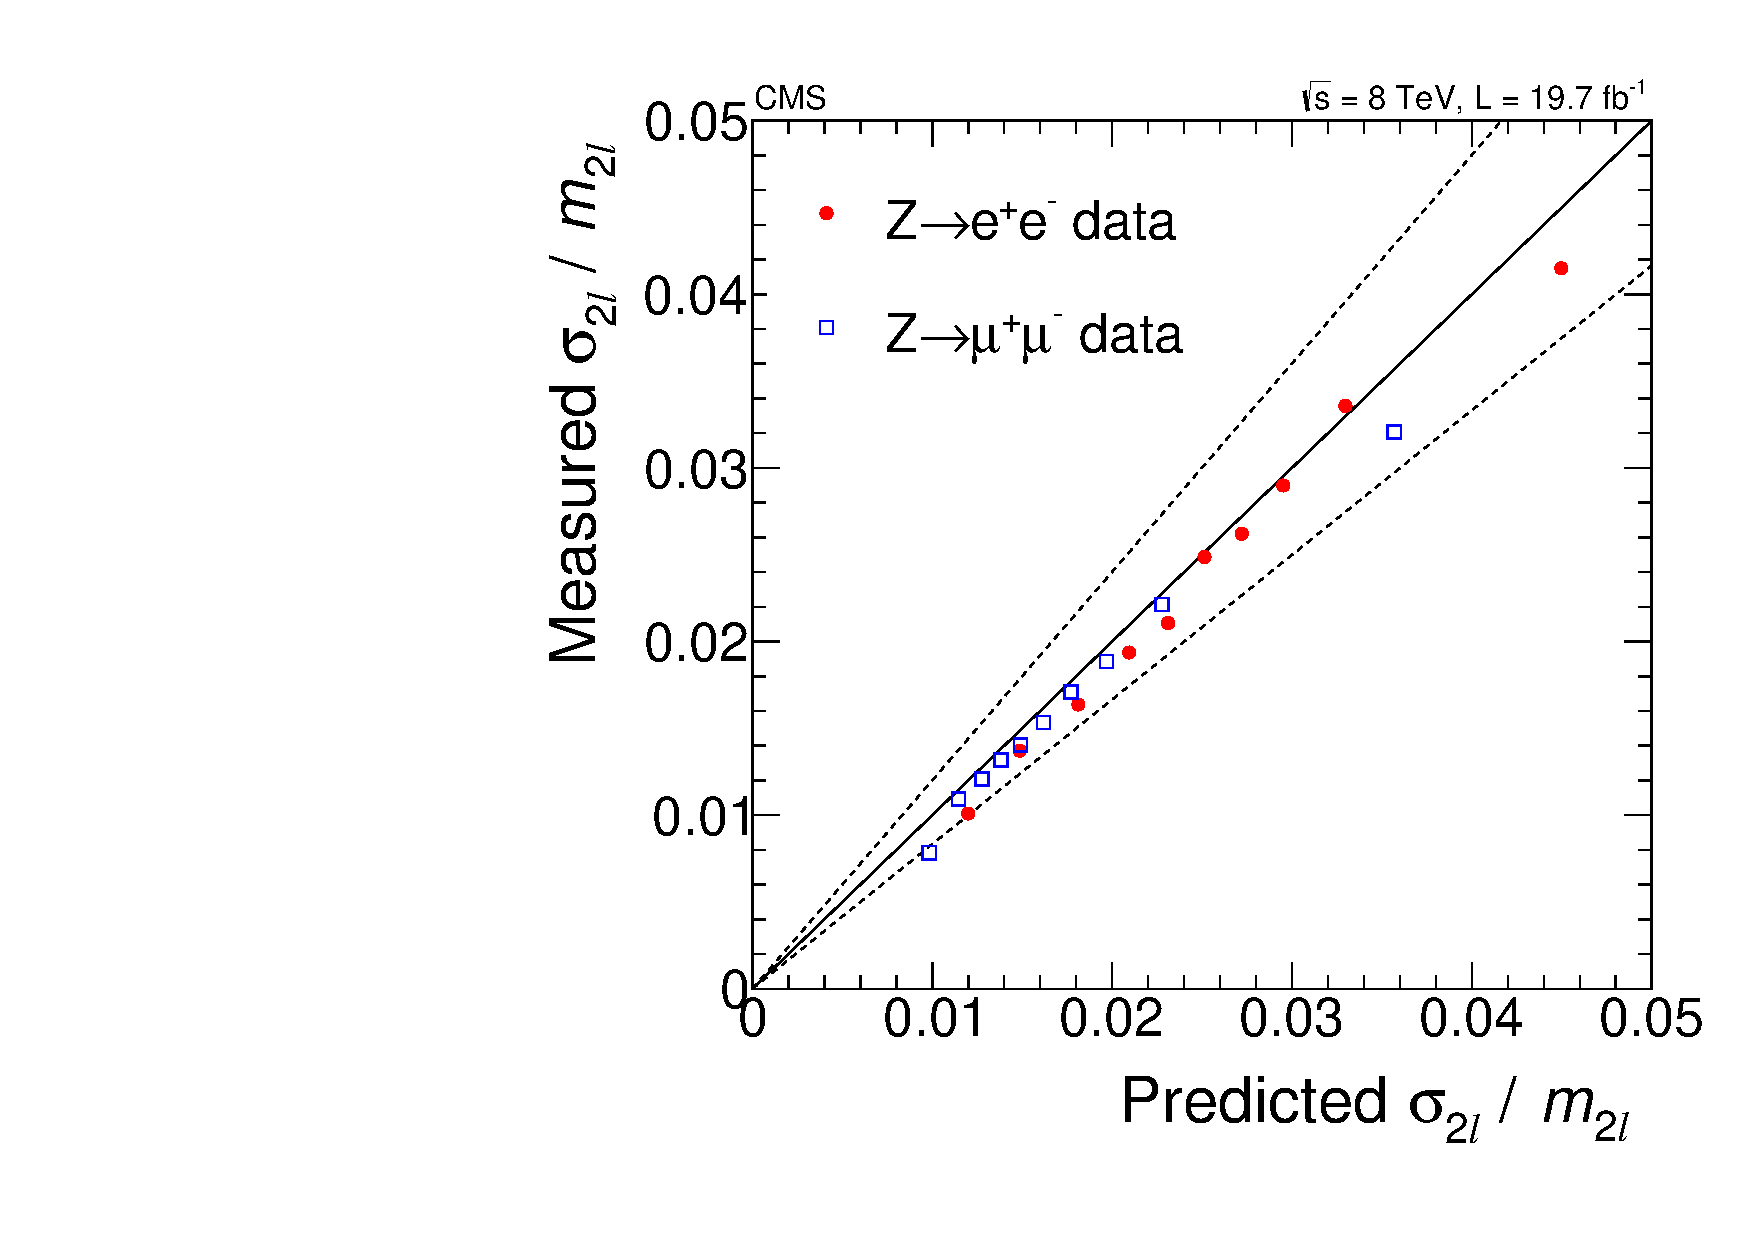
\includegraphics[width=.45\linewidth]{HiggsDiscovery/figures/DmassValid_Z2l.pdf}
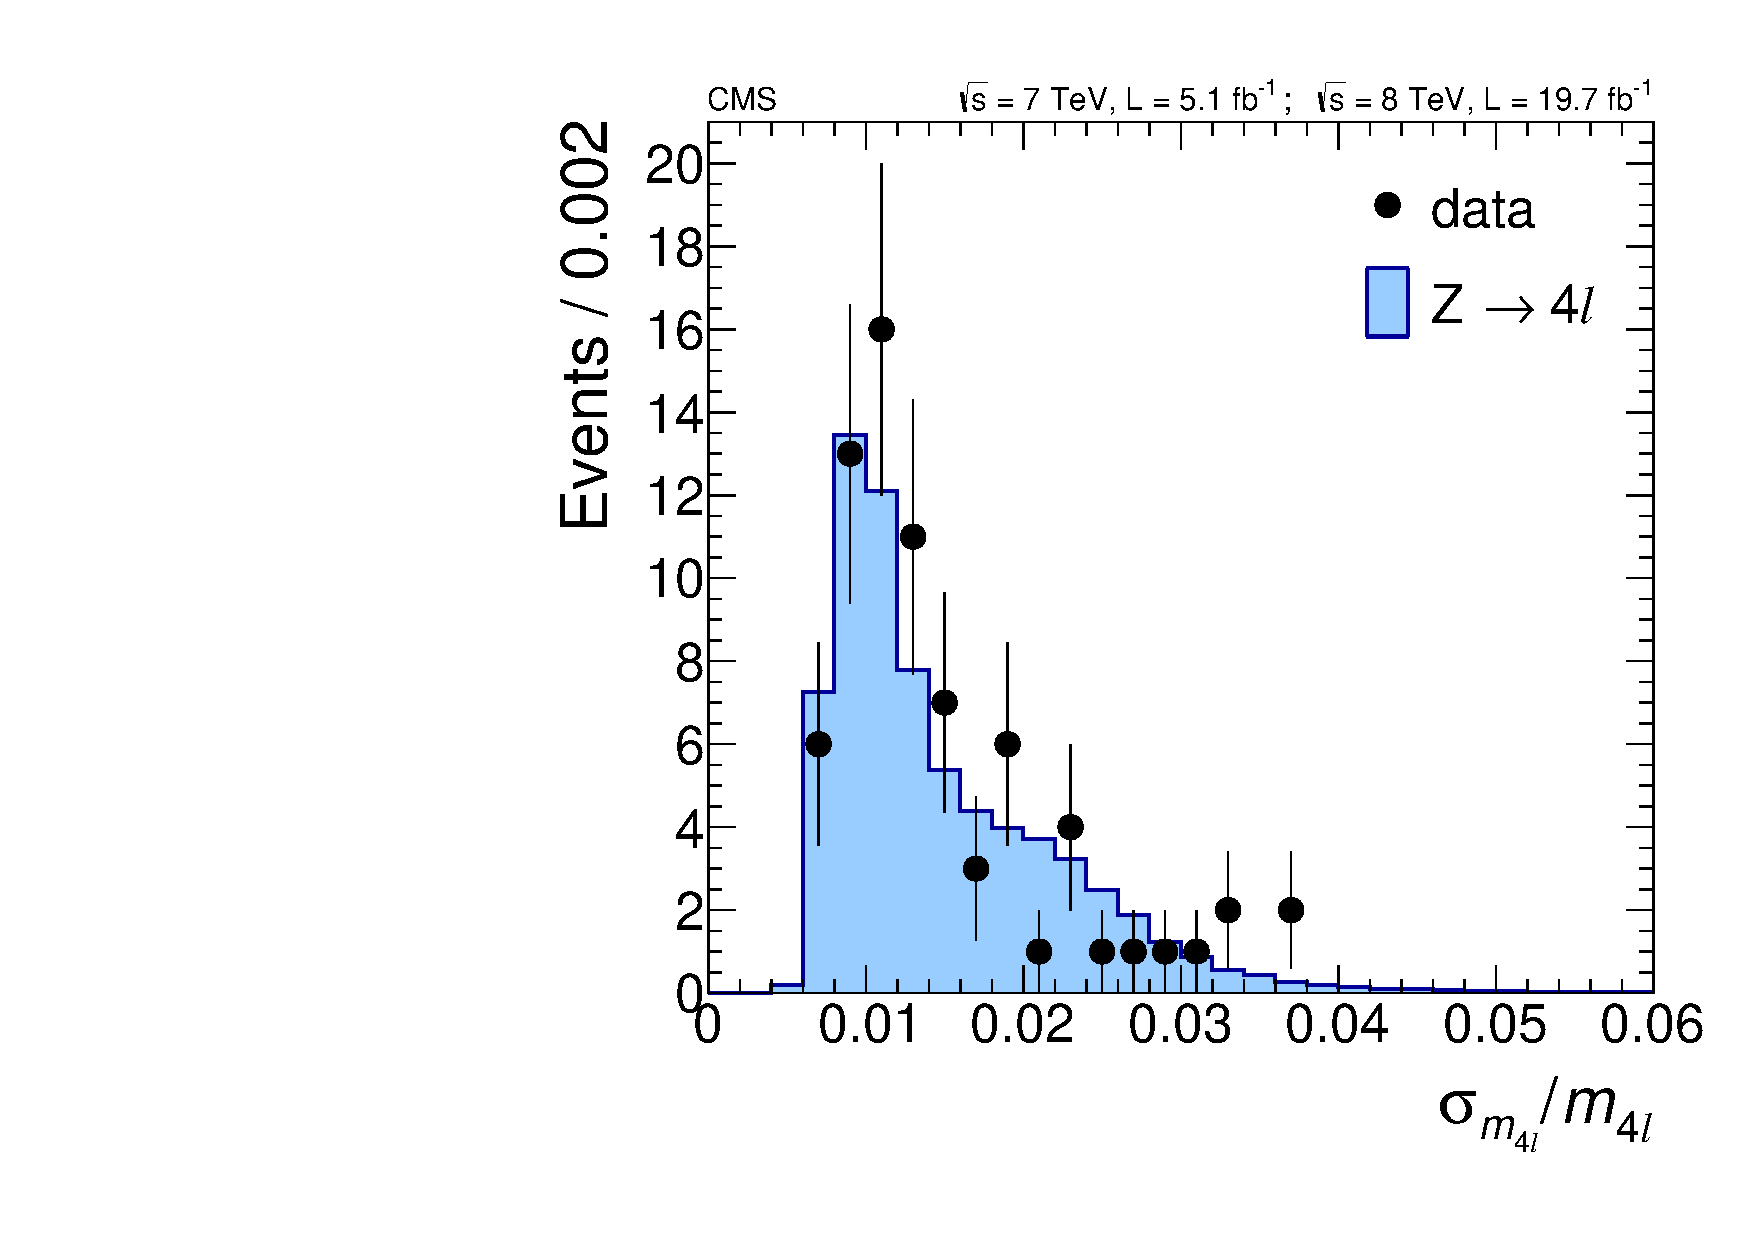
\includegraphics[width=.45\linewidth]{HiggsDiscovery/figures/Dmass_Z4l.pdf}
\caption[Calibration and Closure Test of Per-Event Mass Errors in $4l$]{default}
\label{fig:PerEventMassErrors}
\end{center}
\end{figure}


\section{Results}
\label{sec:ZZ4lResults}

After passing all selection cuts, the total number of observed events with $m_{4l} > 100$ $\rm{GeV}$ for $7$ $\&$ $8$ $\rm{TeV}$ data with background and sample signal estimates are seen in Table~\ref{tbl:ZZ4lEventsFullRange}. The total number of observed events is higher than expected from background alone. When looking at the mass distribution of the $4l$ events in Figures \ref{fig:m4lPlot} and \ref{fig:m4lPlotZoom}, there is a localized excess of events over background expectations near $125$ $\rm{GeV}$. Table~\ref{tbl:ZZ4lEventsNarrowRange} details the number of observed and expected events in this localized region, $121.5 < m_{4l} < 130.5$ $\rm{GeV}$. 

\begin{table}[htbp]
\begin{center}
\begin{tabular}{l|c|c|c|c}
\hline \hline
      Channel         & $4e$ & $2e2\mu$ & $4\mu$ & $4l$  \\
      \hline
      $ZZ$ background  & 77  $\pm$ 10    &  191  $\pm$  25  & 119  $\pm$  15     &  387  $\pm$ 31\\
      $Z + X$  background & 7.4 $\pm$ 1.5   & 11.5  $\pm$ 2.9  & 3.6  $\pm$ 1.5     &  22.6 $\pm$ 3.6  \\
      \hline
      All backgrounds        & 85 $\pm$ 11     & 202  $\pm$ 25    &  123  $\pm$ 15     &  410 $\pm$ 31 \\
      \hline
      $m_H =  500$ $\rm{GeV}$ &  5.2  $\pm$  0.6  & 12.2  $\pm$  1.4 &   7.1  $\pm$  0.8  &  24.5 $\pm$ 1.7  \\
      $m_H =  800$ $\rm{GeV}$ &  0.7  $\pm$  0.1  &  1.6  $\pm$  0.2 &   0.9  $\pm$  0.1  &  3.1  $\pm$ 0.2 \\
      \hline
      Observed  & 89 & 247 & 134 & 470\\
\hline \hline
\end{tabular}
\caption[Number of Observed $4l$ Events in $100 < m_{4l} < 1000$ $\rm{GeV}$]{Total number of observed and estimated events after all selection cuts for $m_{4l} > 100$ $\rm{GeV}$. Estimates for signal and irreducible $ZZ$ background come from Monte Carlo simulations. Irreducible $Z+X$ background estimates are data driven.
\label{tbl:ZZ4lEventsFullRange}}
\end{center}
\end{table}

\begin{figure}[htbp]
\begin{center}
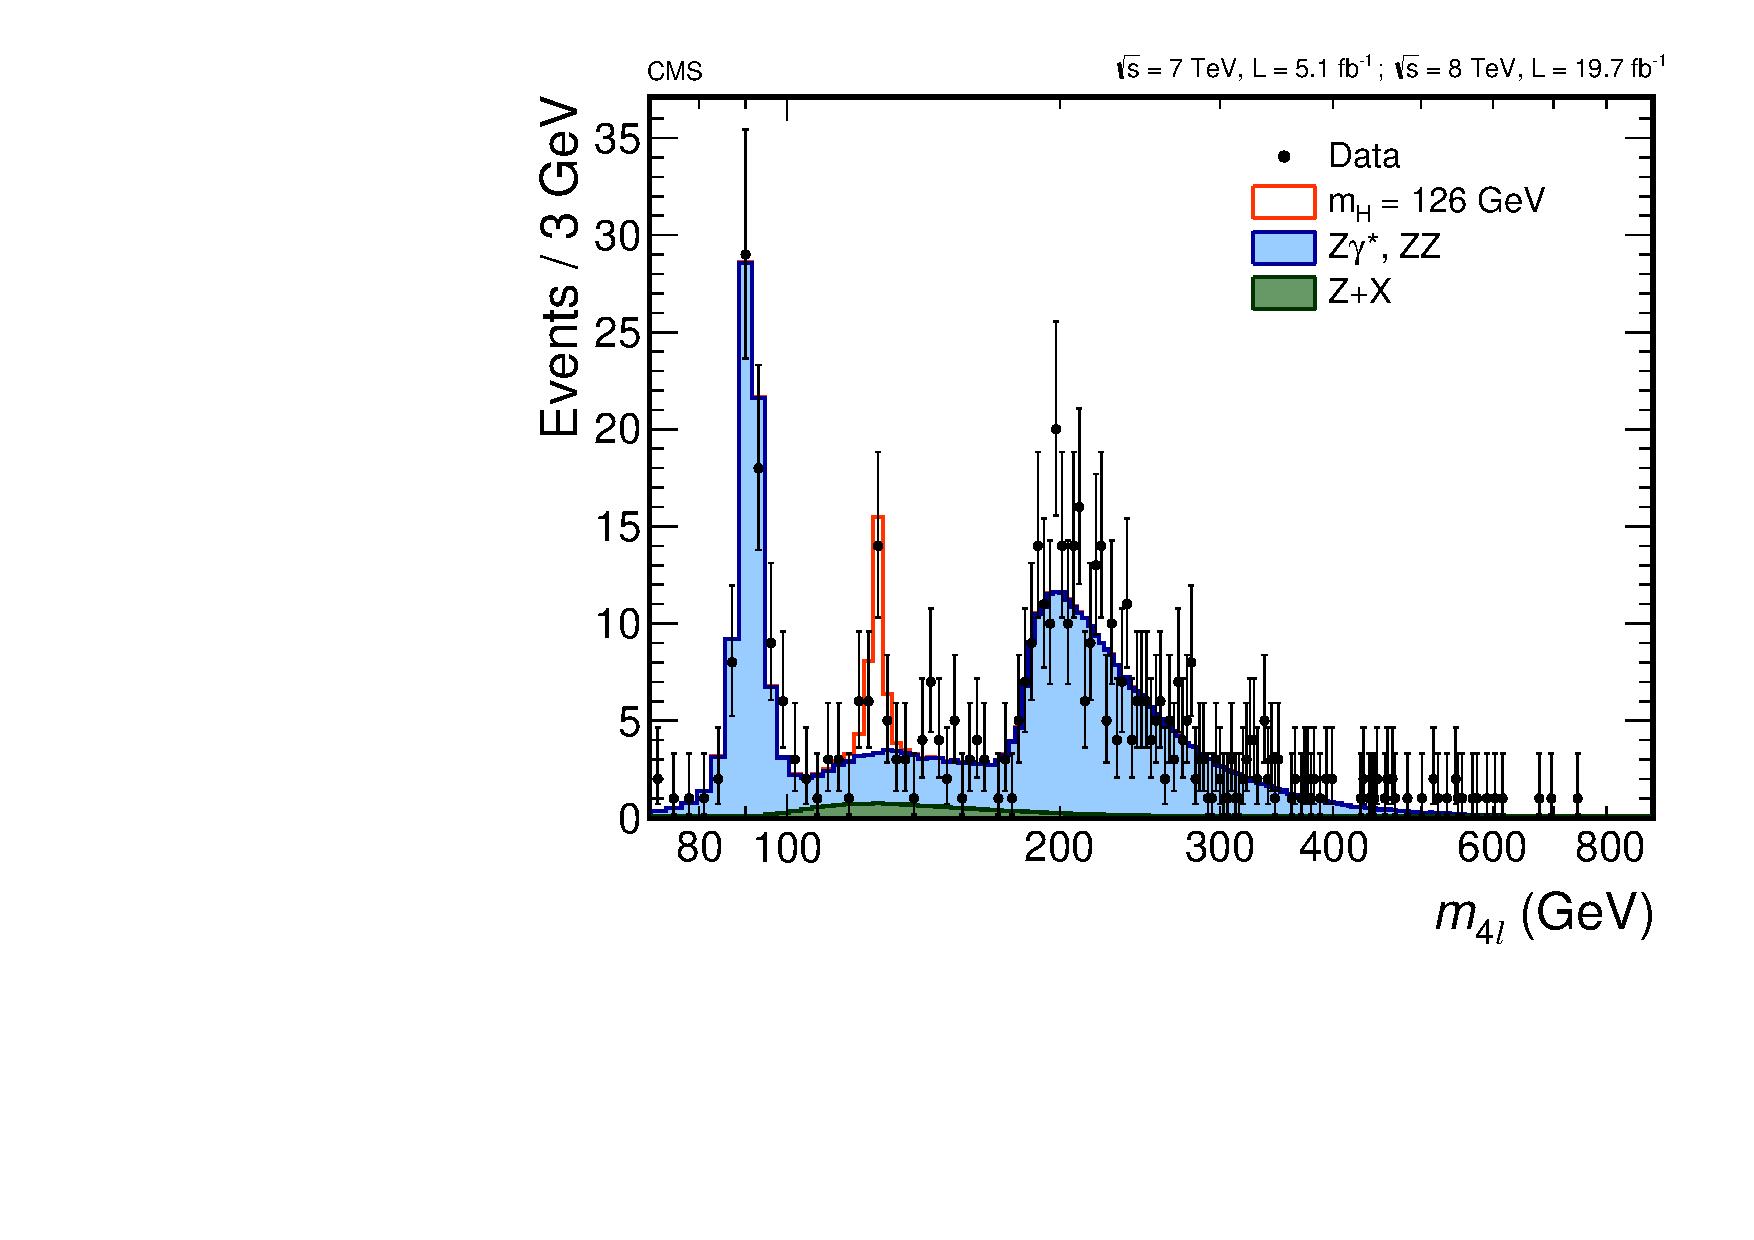
\includegraphics[width=.7\linewidth]{HiggsDiscovery/figures/ZZMass_7Plus8TeV_70-1000_3GeV.pdf}
\caption[$m_{4l}$ Distributions of $4l$ Events]{Distribution of $m_{4l}$ for combined $7$  $\&$ $8$ $\rm{TeV}$ data, with expected distributions reducible $Z+X$ (green) and irreducible $Z\gamma^{*}/ZZ$ (blue) backgrounds for $70< m_{4l} < 1000$ $\rm{GeV}$. Peaks for $Z\rightarrow 4l$ and $ZZ\rightarrow 4l$ are observed. An excess of events appears near $m_{4l} = 126$ $\rm{GeV}$ (red).}
\label{fig:m4lPlot}
\end{center}
\end{figure}

\begin{figure}[htbp]
\begin{center}
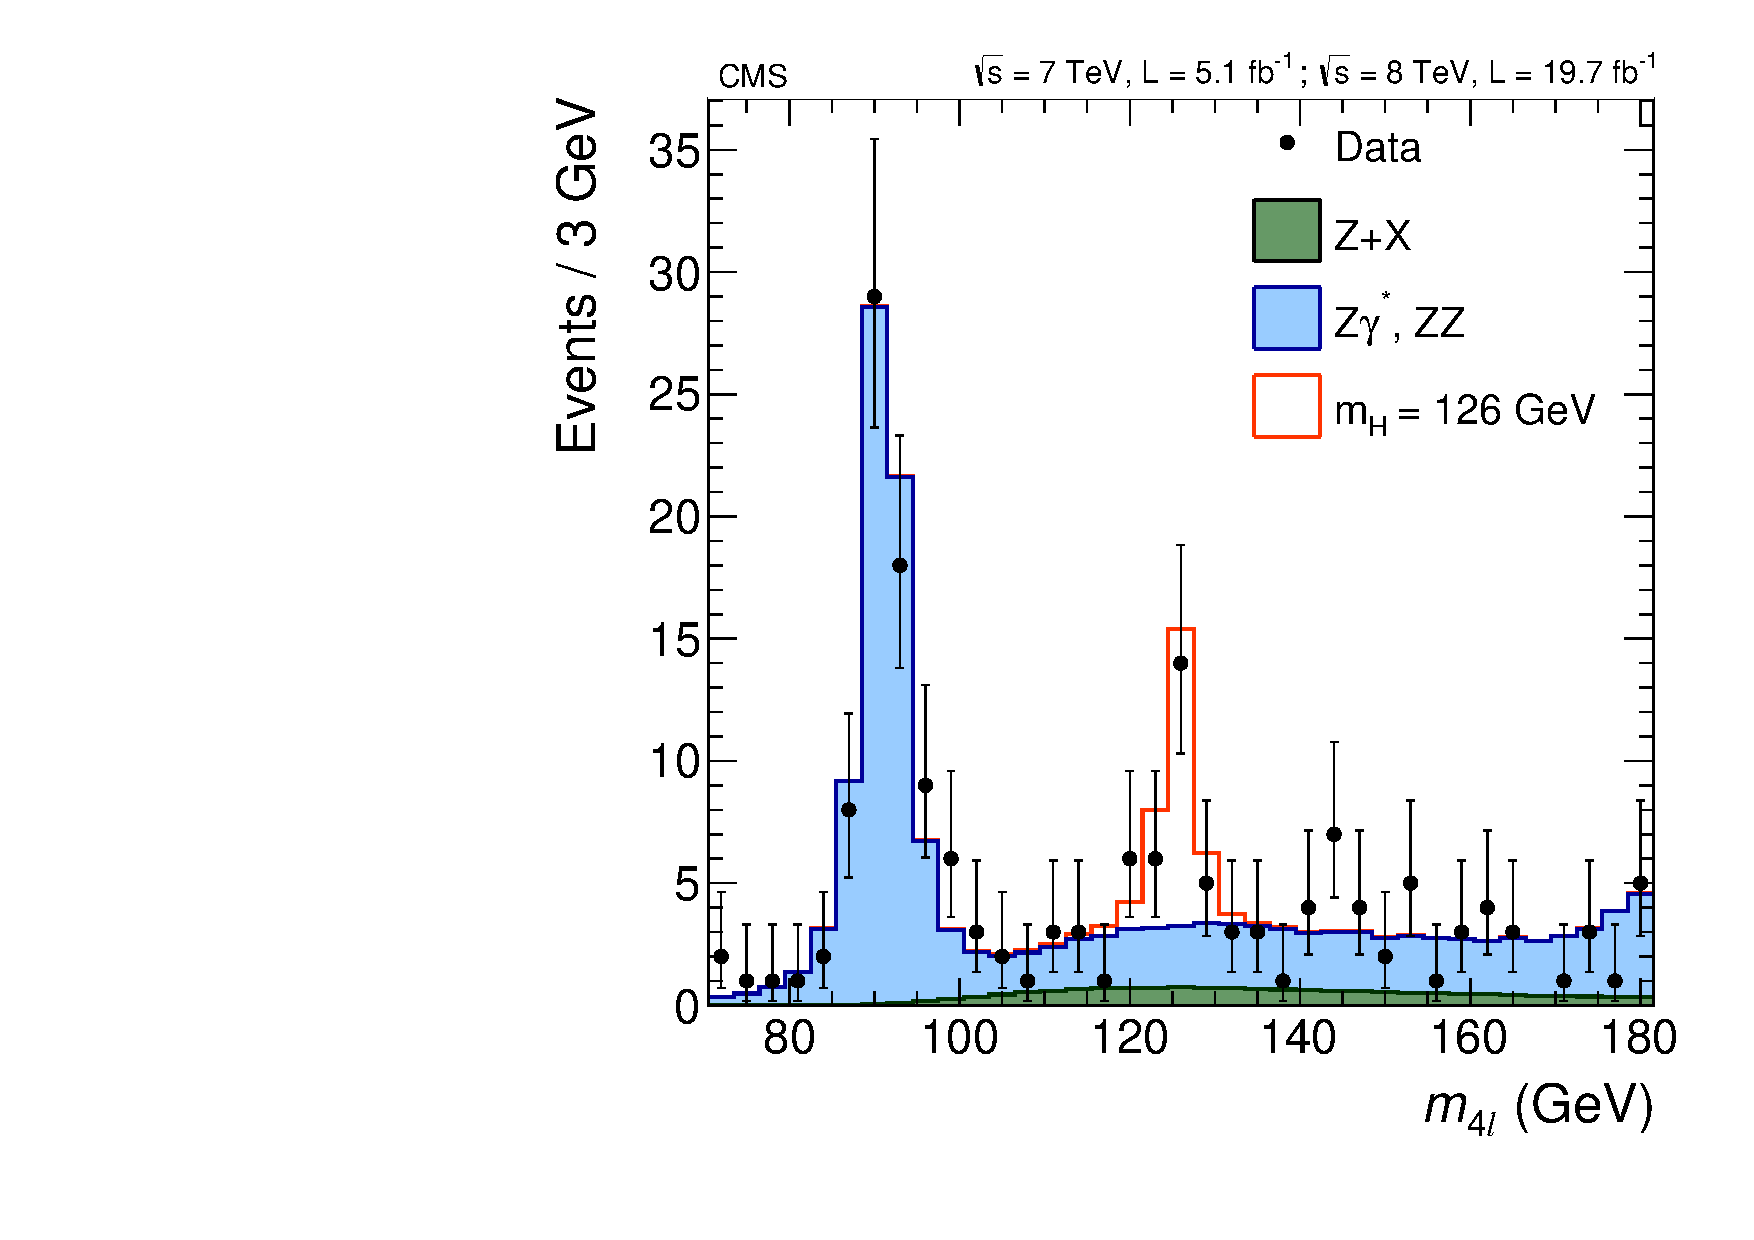
\includegraphics[width=.7\linewidth]{HiggsDiscovery/figures/ZZMass_7Plus8TeV_70-180_3GeV.pdf}
\caption[$m_{4l}$ Distributions of $4l$ Events, $m_{4l}<180$ $\rm{GeV}$]{Distribution of $m_{4l}$ for combined $7$  $\&$ $8$ $\rm{TeV}$ data, with expected distributions reducible $Z+X$ (green) and irreducible $Z\gamma^{*}/ZZ$ (blue) backgrounds for $70< m_{4l} < 180$ $\rm{GeV}$. Peaks for $Z\rightarrow 4l$ and $ZZ\rightarrow 4l$ are observed. An excess of events appears near $m_{4l} = 126$ $\rm{GeV}$ (red).}
\label{fig:m4lPlotZoom}
\end{center}
\end{figure}

\begin{table}[htbp]
\begin{center}
\begin{tabular}{l|c|c|c|c}
\hline \hline
      Channel        & $4e$ & $2e2\mu$ & $4\mu$  & $4l$ \\
      \hline
      $ZZ$ background &  1.1  $\pm$  0.1  &  3.2  $\pm$  0.2  &  2.5  $\pm$  0.2  &  6.8 $\pm$ 0.3  \\
      $Z + X$ background &  0.8  $\pm$  0.2  &  1.3  $\pm$  0.3  &  0.4  $\pm$  0.2  &  2.6 $\pm$ 0.4 \\
      \hline
      All backgrounds            &  1.9  $\pm$  0.2   &  4.6  $\pm$ 0.4  & 2.9  $\pm$ 0.2  & 9.4  $\pm$ 0.5\\
      \hline
      $m_H =  125$ $\rm{GeV}$ &  3.0  $\pm$  0.4  &  7.9  $\pm$  1.0  &  6.4  $\pm$  0.7  & 17.3  $\pm$ 1.3 \\
      $m_H =  126$ $\rm{GeV}$ &  3.4  $\pm$  0.5  &  9.0  $\pm$  1.1  &  7.2  $\pm$  0.8  & 19.6  $\pm$ 1.5 \\
      \hline
      Observed  & 4 & 13 & 8 & 25 \\
\hline \hline
\end{tabular}
\caption[Number of Observed $4l$ Events in $121.5 < m_{4l} < 130.5$ $\rm{GeV}$]{Total number of observed and estimated events after all selection cuts for $121.5 < m_{4l} < 130.5$ $\rm{GeV}$. Estimates for signal and irreducible $ZZ$ background come from Monte Carlo simulations. Irreducible $Z+X$ background estimates are data driven.
\label{tbl:ZZ4lEventsNarrowRange}}
\end{center}
\end{table}

To test whether any deviation from the background is in agreement with the Higgs hypothesis and not just localized statistical fluctuations, we must evaluate the likelihood at different mass points. The unbinned distributions of the kinematics of $4l$ events that pass selection are examined at 187 different mass points between $100\leq m_{H} \leq 1000$ $\rm{GeV}$, where each mass point has a window optimized for the expected Higgs width at that mass and/or detector resolution. A simultaneous likelihood fit, following the procedure suggested by \cite{}, is used to compute exclusion limits and significance of any excess.

Using a modified frequentist construction\footnote{A Bayesian approach \cite{} is also consistent with all reported results.} $\mathrm{CL_s}$ \cite{} to report limits, the 95\% confidence level upper limit on the \textit{signal strength} ($\mu$), where $\mu=\sigma_{95\%}/\sigma_{SM}$: the ratio of the produced cross section to the SM-like cross section, is calculated for a large pseudo-dataset. This means that for expected $\mu>1$, the upper limit is higher than the SM-like cross section, so it is not possible to distinguish an excess. The corollary is that the region with expected $\mu\leq1$ is the \textit{expected exclusion range}. The median of this upper limit, with $\pm2\sigma$ bands, defines the range of expectations for the background-only hypothesis. Then, the upper-limit of the signal strength can be computed using the observed events. Any mass points within the range of expectations for the background-only hypothesis are in agreement and thus exclude the existence of a signal where $\mu\leq1$.

For the $4l$ events, the observed and excluded limits are seen in the left plot of Fig.~\ref{fig:ExclusionLimits}. A SM-like boson was expected to be excluded in the mass range $115< m_H <740$ $\rm{GeV}$. The observed 95\% CL exclusion limit is the mass ranges $114.5<m_H<119.0$ $\rm{GeV}$ and $129.5<m_H<832.0$ $\rm{GeV}$. In regions where a signal is not excluded, the standard cutoff used to consider an excess a discovery is a local probability $5\sigma$ above\footnote{Any substantial lack of events would be considered a mismodeling of the background.} the background-only median. The reason for the stringent limit is the \textit{look-elsewhere effect}: the mass of the Higgs is unknown, so when probing more mass points, the odds of any one point having an excess over $2\sigma$ increases. In the right plot of Fig.~\ref{fig:ExclusionLimits}, a local significance of $6.8\sigma$ occurs at $m_H=125.7$ $\rm{GeV}$. For a Higgs-like boson at that mass, the expected significance is $6.8\sigma$.

\begin{figure}[htbp]
\begin{center}
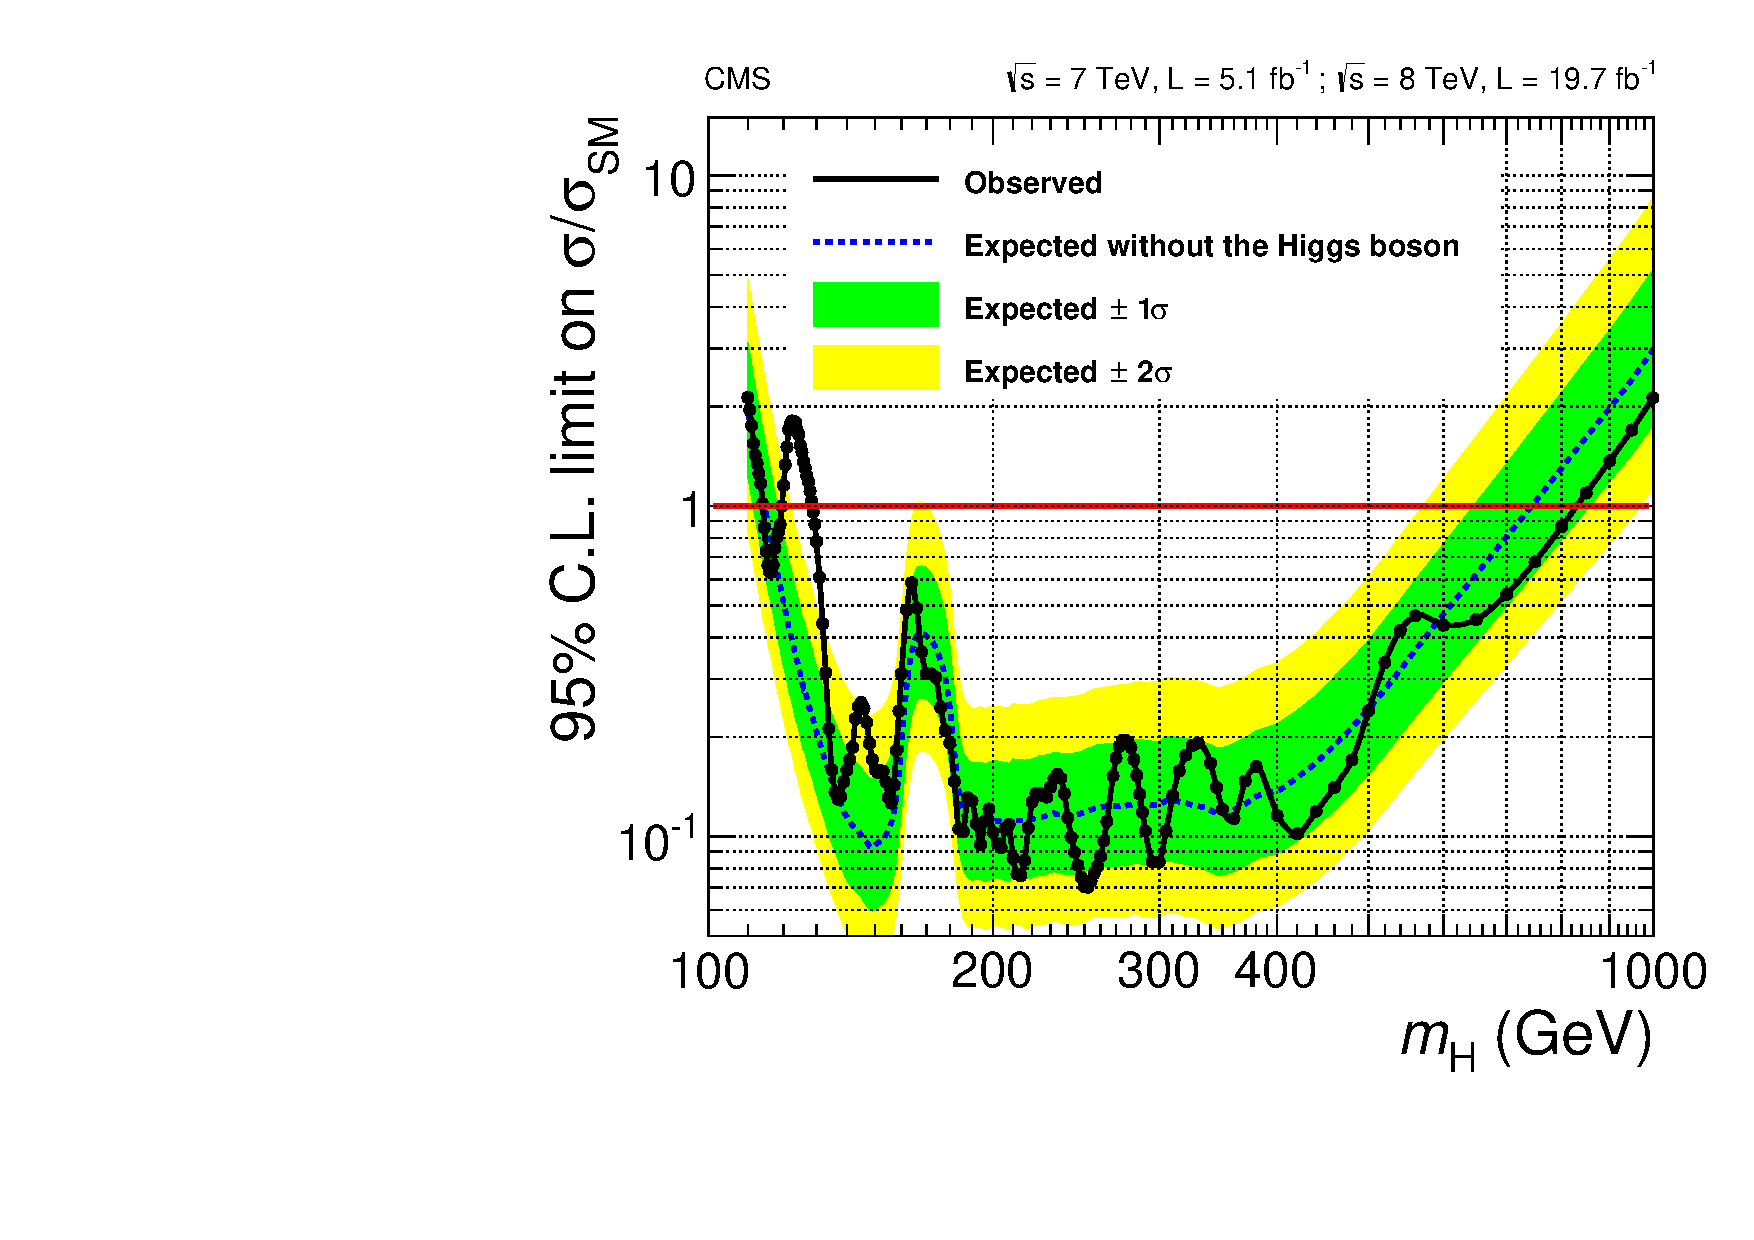
\includegraphics[width=.45\linewidth]{HiggsDiscovery/figures/UpperLimit_ASCLS_7p8TeV_wholeMass_Final2_2l2tau.pdf}
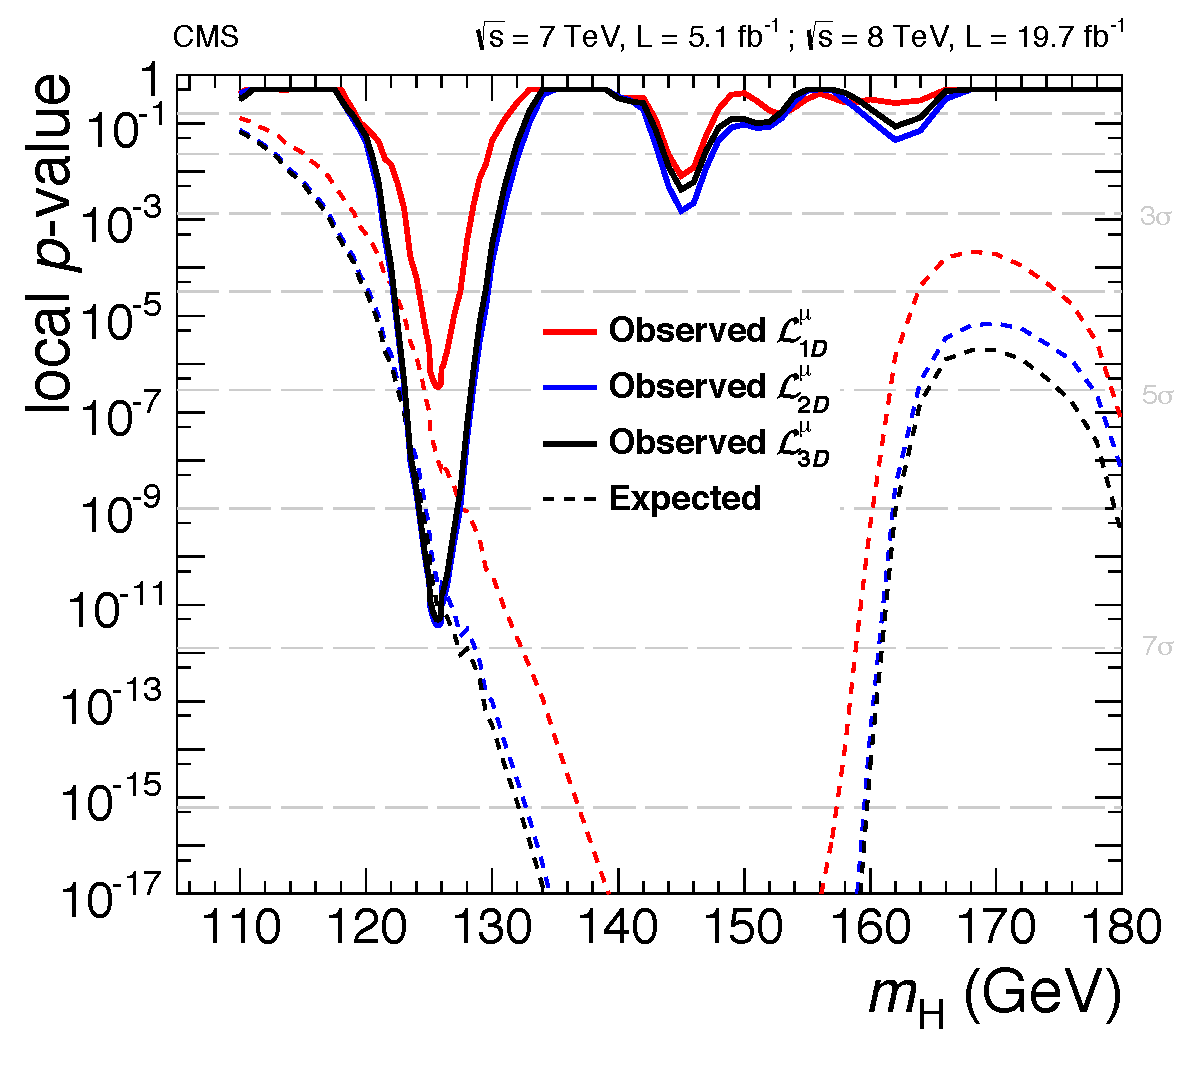
\includegraphics[width=.45\linewidth]{HiggsDiscovery/figures/Pvals_PLP_lowMass_1D2D3D_Final3_no2l2tau_7p8sep.pdf}
\caption[Exclusion Limits and Local Probabilities for $4l$ Events]{On left, expected and observed 95\% CL upper limits on signal strength as functions of $m_{H}$, using $7\&8$ $\rm{TeV}$ data. Dashed black line is the expected limit with 68\% and 95\% ranges of expectation in green and yellow bands, respectively. Observed limit is solid black line, where the excluded range is $114.5<m_H<119.0$ $\rm{GeV}$ and $129.5<m_H<832.0$ $\rm{GeV}$. On right, the expected (dashed) and observed (solid) local probability values for $110<m_{H}<180$ $\rm{GeV}$. Black lines indicate full 3D likelihoods, red and blue are cross checks using 1D $m_{4l}$ and 2D $(m_{4l},D_{\rm{bkg}}^{\rm{kin}})$ likelihoods, respectively. Horizontal dashed lines reinterpret probability in terms of number of $\sigma$. An observed (expected) local significance of $6.8\sigma$ $(6.7\sigma)$ occurs at $m_H=125.7$ $\rm{GeV}$.}
\label{fig:ExclusionLimits}
\end{center}
\end{figure}

To emphasize the discovery, the distributions of the events for $D_{\rm{bkg}}^{\rm{kin}}$ and $p_T$ or $D_{jet}$ are plotted over expectations. For the decay kinematics, as seen in Fig.~\ref{fig:Dbkg_2D_Results}, the $4l$ events are plotted over heat maps of background-only $D_{\rm{bkg}}^{\rm{kin}}$ distributions. In Fig.~\ref{fig:Dbkg_2D_Results_Peak}, a number of events near $m_{4l}=126$ $\rm{GeV}$ have higher values of $D_{\rm{bkg}}^{\rm{kin}}$ in agreement with the expected distribution of background plus $m_H=126$ $\rm{GeV}$ signal. In Fig.~\ref{fig:pT_Results}, the $p_T$ distribution of the events in the low mass region are plotted over the expected distributions, where the events appear to have slightly higher $p_T$ than expected. In Fig.~\ref{fig:Fisher_Results}, nearly all dijet events occur around $m_{4l}=126$ $\rm{GeV}$.

\begin{figure}[htbp]
\begin{center}
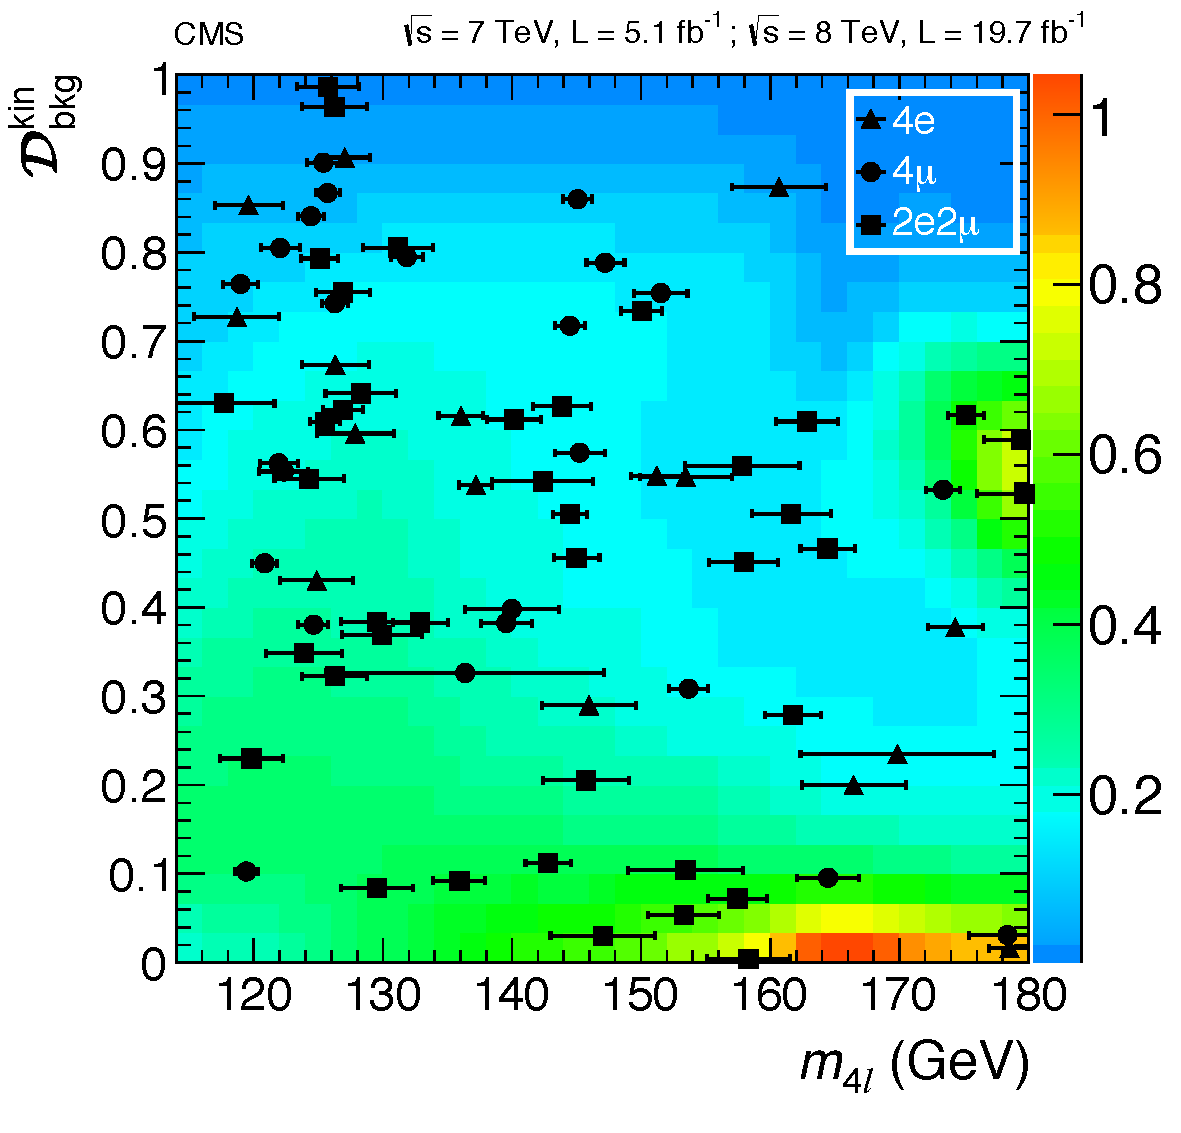
\includegraphics[width=.45\linewidth]{HiggsDiscovery/figures/KD_vs_m4l_lowMass_Back.pdf}
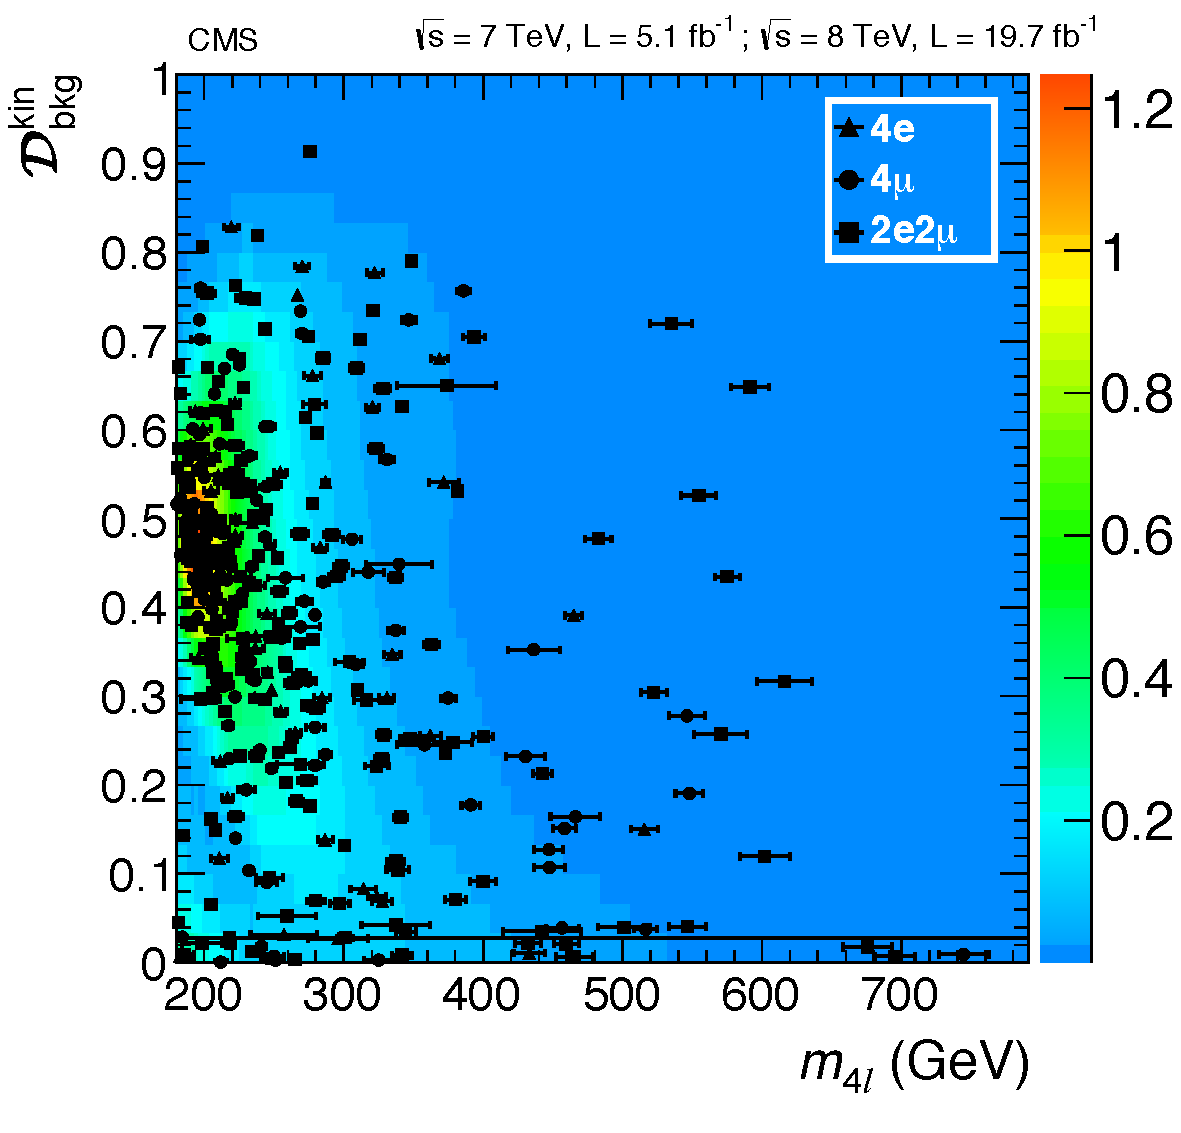
\includegraphics[width=.45\linewidth]{HiggsDiscovery/figures/KD_vs_m4l_highMass_Back.pdf}
\caption[Observed $D_{\rm{bkg}}^{\rm{kin}}$ Distributions for $4l$ Events]{$D_{\rm{bkg}}^{\rm{kin}}$ v $m_{4l}$ distributions for $4e$ (triangles), $4\mu$ (circles), and $2e2\mu$ (squares) events with $115 < m_{4l} < 180$ $\rm{GeV}$ (left) and $180 < m_{4l} < 800$ $\rm{GeV}$ (left). Events have per event mass errors. Heat maps correspond to expected distributions for background only.}
\label{fig:Dbkg_2D_Results}
\end{center}
\end{figure}

\begin{figure}[htbp]
\begin{center}
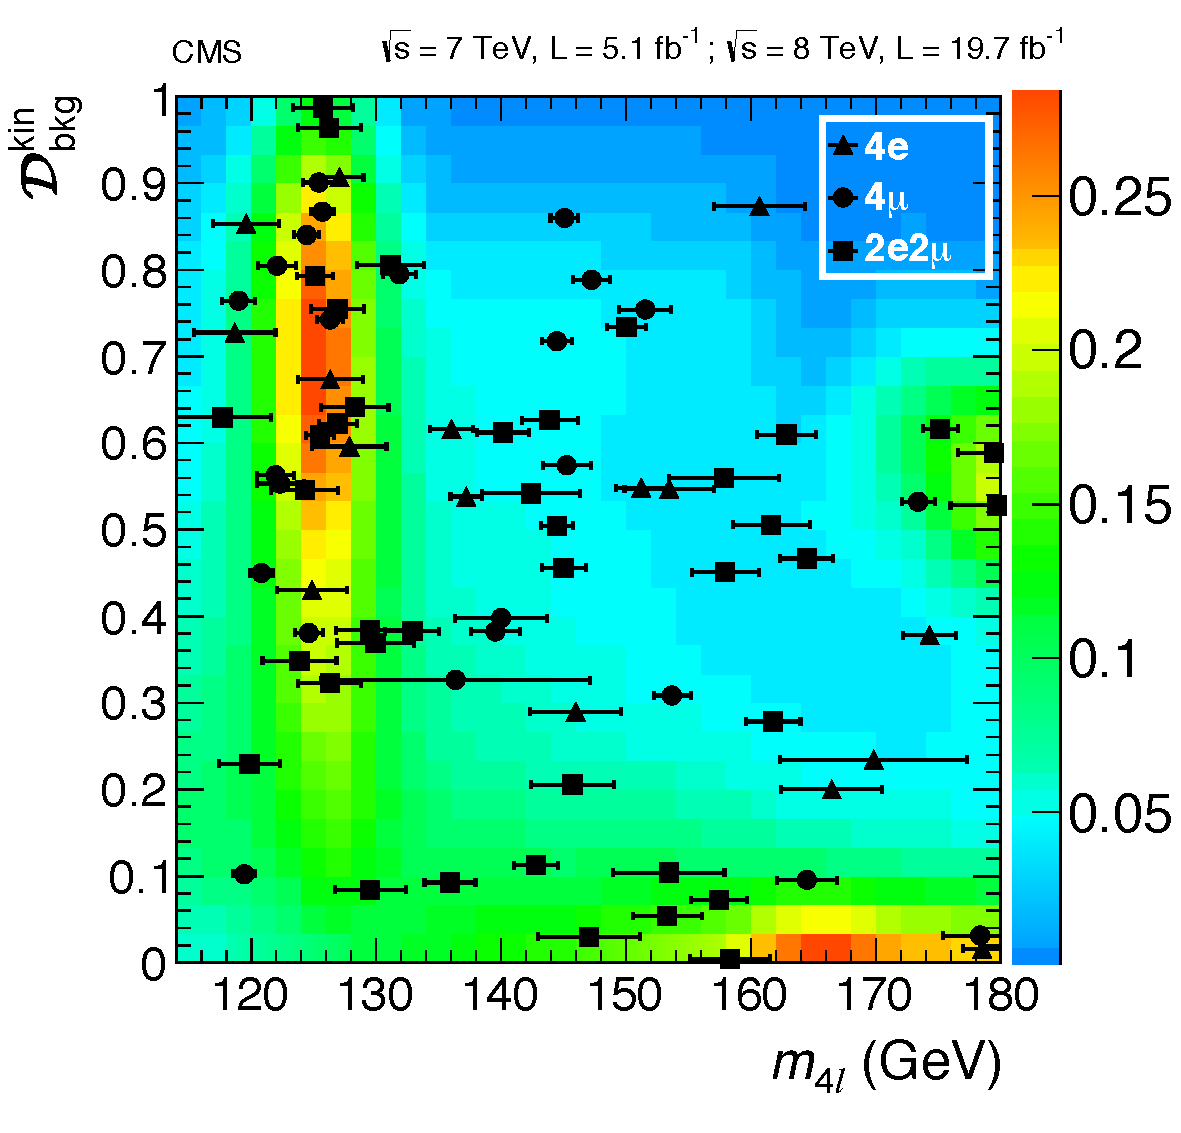
\includegraphics[width=.45\linewidth]{HiggsDiscovery/figures/KD_vs_m4l_lowMass_Signal.pdf}
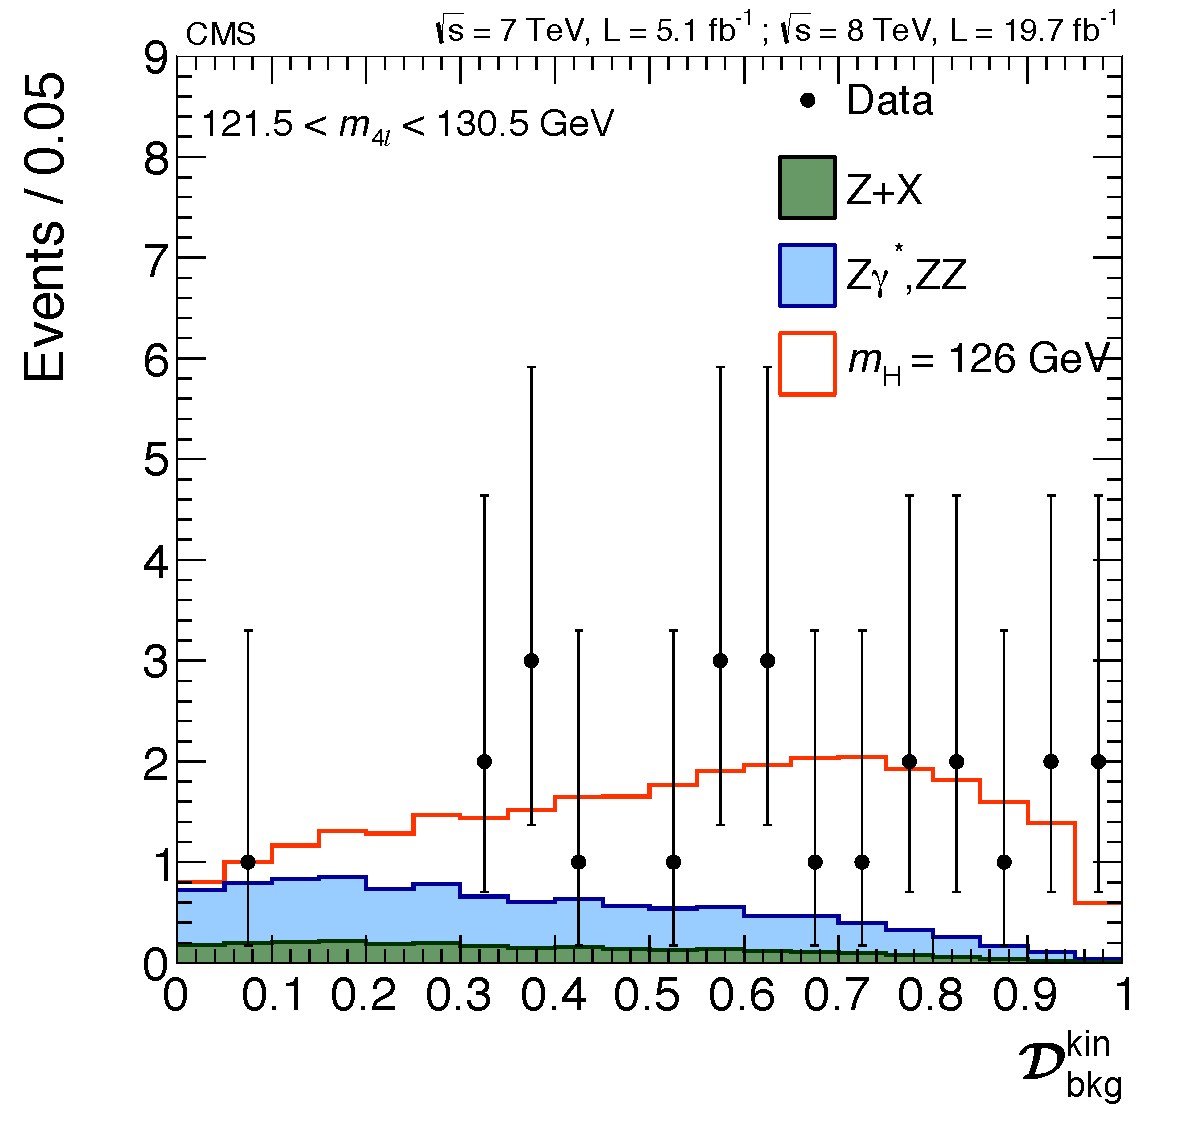
\includegraphics[width=.45\linewidth]{HiggsDiscovery/figures/KDPeak.pdf}
\caption[Observed $D_{\rm{bkg}}^{\rm{kin}}$ Distributions for Low Mass $4l$ Events With Signal Expectations]{On left, $D_{\rm{bkg}}^{\rm{kin}}$ v $m_{4l}$ distributions for $4e$ (triangles), $4\mu$ (circles), and $2e2\mu$ (squares) events with $115 < m_{4l} < 180$ $\rm{GeV}$. Events have per event mass errors. Heat map corresponds to expected distributions for background and $m_H = 126$ $\rm{GeV}$ signal. On right, projection of $D_{\rm{bkg}}^{\rm{kin}}$ for events and background expectations in $121.5 < m_{4l} < 130.5$ $\rm{GeV}$ range.}
\label{fig:Dbkg_2D_Results_Peak}
\end{center}
\end{figure}

\begin{figure}[htbp]
\begin{center}
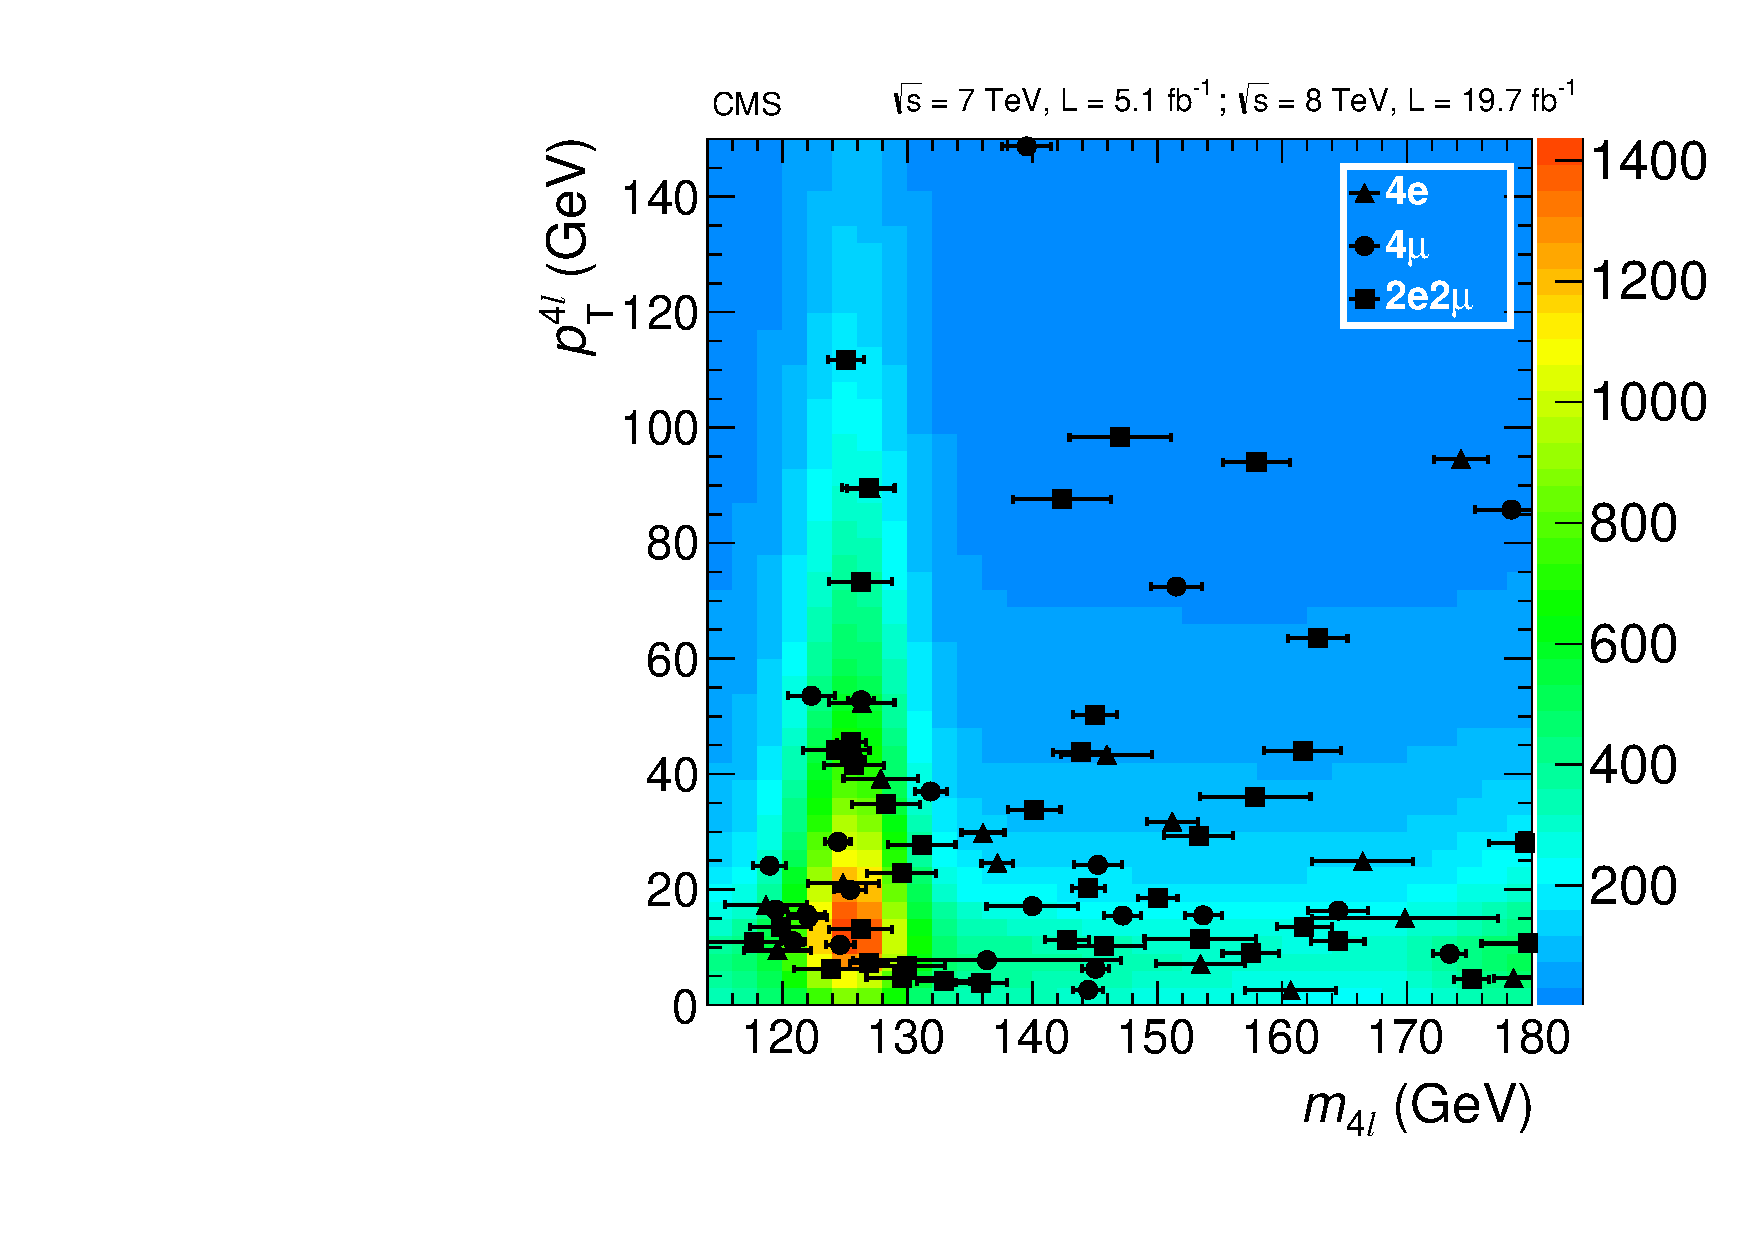
\includegraphics[width=.45\linewidth]{HiggsDiscovery/figures/M4l_vs_pT_all.pdf}
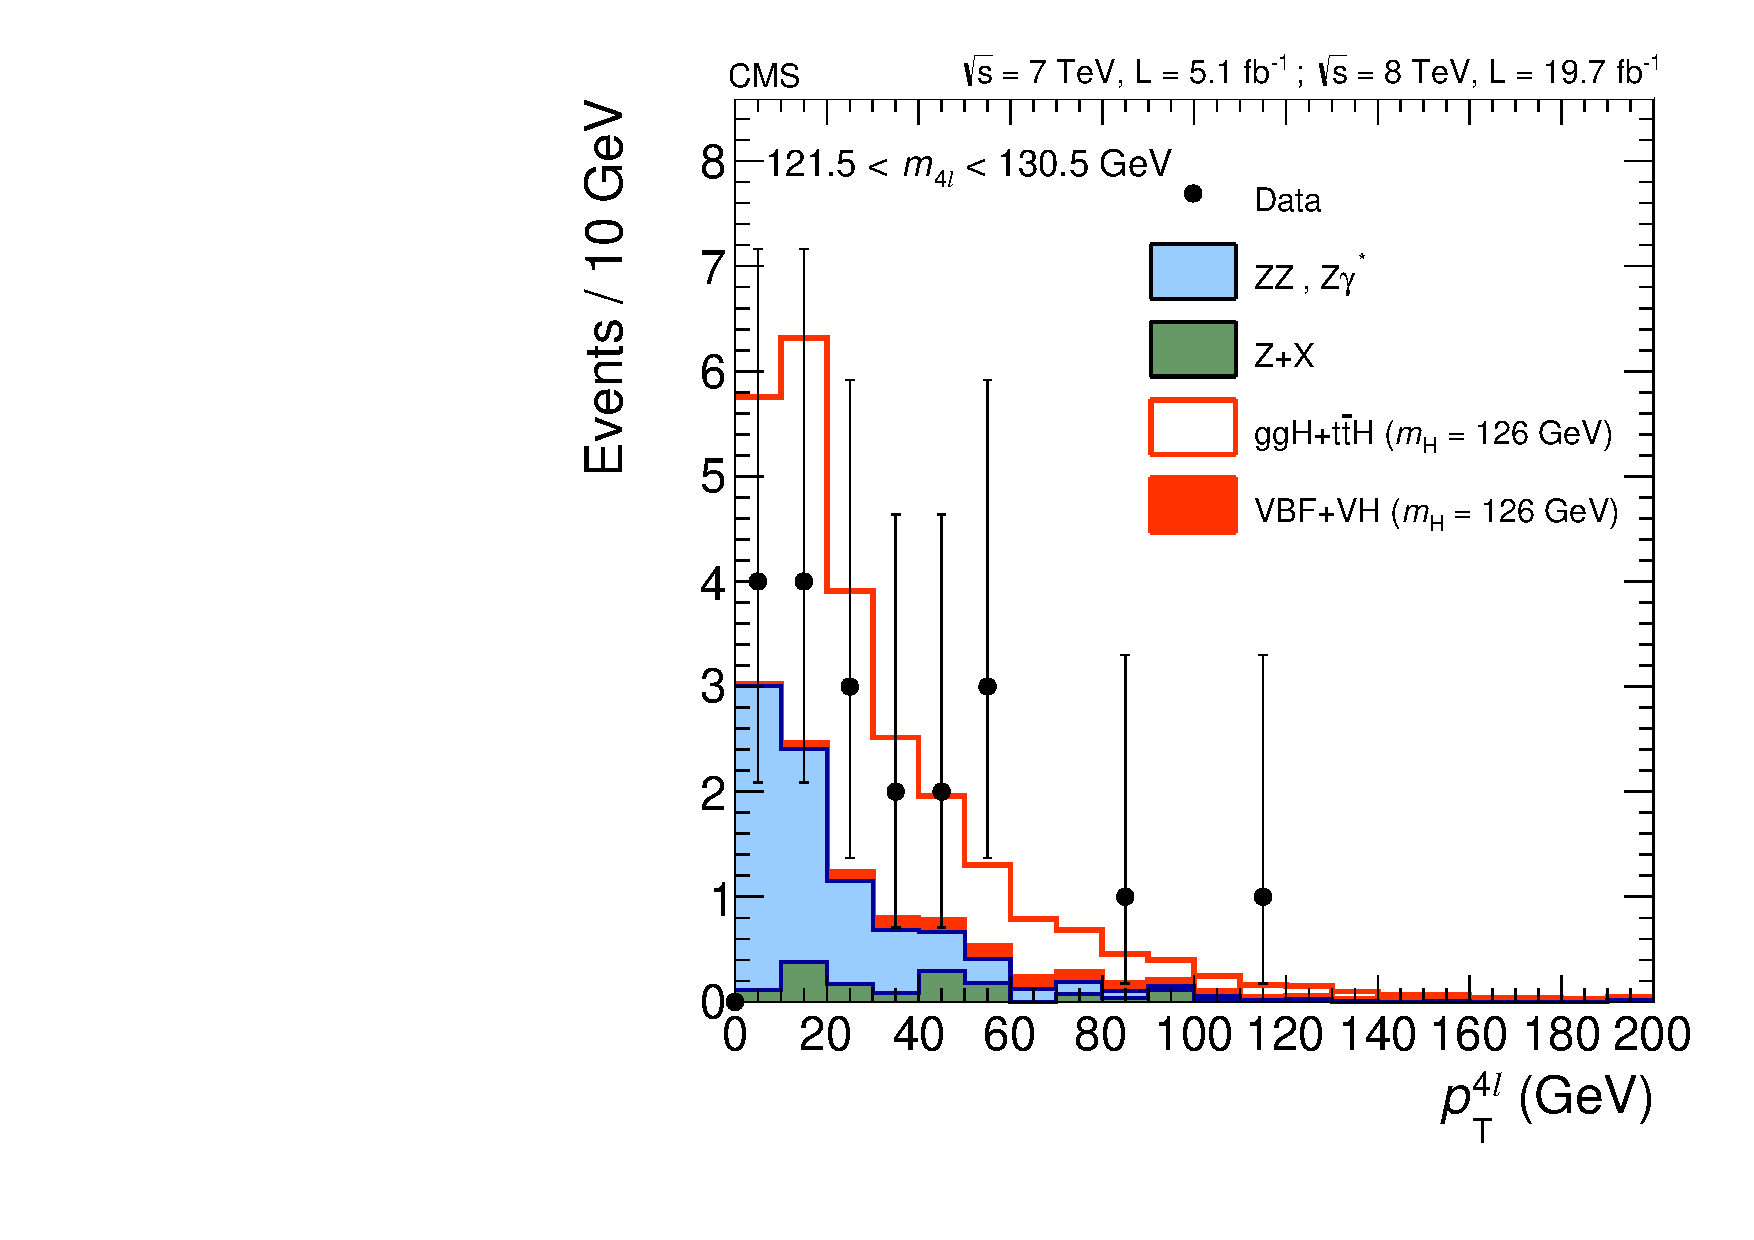
\includegraphics[width=.45\linewidth]{HiggsDiscovery/figures/PT01JetPeak.pdf}
\caption[Observed $p_T$ Distributions for Low Mass $4l$ Events With Signal Expectations]{On left, $p_T$ v $m_{4l}$ distributions for $4e$ (triangles), $4\mu$ (circles), and $2e2\mu$ (squares) events with $115 < m_{4l} < 180$ $\rm{GeV}$. Events have per event mass errors. Heat map corresponds to expected distributions for background and $m_H = 126$ $\rm{GeV}$ signal. On right, projection of $p_T$ for events and background expectations in $121.5 < m_{4l} < 130.5$ $\rm{GeV}$ range. Expected signal is split into fermionic (ggF and $t\bar{t}H$) and bosonic (VBF + VH) couplings.}
\label{fig:pT_Results}
\end{center}
\end{figure}

\begin{figure}[htbp]
\begin{center}
\includegraphics[width=.45\linewidth]{HiggsDiscovery/figures/M4l_vs_Fisher_all.pdf}
\includegraphics[width=.45\linewidth]{HiggsDiscovery/figures/FisherPeak.pdf}
\caption[Observed $D_{jet}$ Distributions for Low Mass $4l$ Events With Signal Expectations]{On left, $D_{jet}$ v $m_{4l}$ distributions for $4e$ (triangles), $4\mu$ (circles), and $2e2\mu$ (squares) events with $115 < m_{4l} < 180$ $\rm{GeV}$. Events have per event mass errors. Heat map corresponds to expected distributions for background and $m_H = 126$ $\rm{GeV}$ signal. On right, projection of $D_{jet}$ for events and background expectations in $121.5 < m_{4l} < 130.5$ $\rm{GeV}$ range. Expected signal is split into fermionic (ggF and $t\bar{t}H$) and bosonic (VBF + VH) couplings.}
\label{fig:Fisher_Results}
\end{center}
\end{figure}

The most pressing properties of the discovered particle to be measured are its mass and its signal strength. If it is the SM Higgs, as we have seen in Sec.~\ref{sec:pheno} the mass determines many of its other properties. In the region near $m_{4l}=125$ $\rm{GeV}$, a different 3D likelihood is built using the same $m_{4l}$ distributions and two-dimensional $(m_{4l},\mathcal{D}_{\rm{bkg}}^{\rm{kin}})$ templates, but replacing the production templates with templates for the per-event mass errors\footnote{Similar to other 2D templates, a distribution from MC (or control region for $Z+X$), was fit using an analytic function.} using a discriminant $\mathcal{D}_{\rm{m}}=\sigma_{4l}/m_{4l}$. The likelihood scan using this technique can be seen in Fig.~\ref{fig:MassLikelihood}. The measured mass is $m_H = 125.6 \pm 0.4(\rm{stat}) \pm 0.2(\rm{syst})$ $\rm{GeV}$ where the errors refer to the statistical and systematic uncertainties, respectively.

\begin{figure}[htbp]
\begin{center}
\includegraphics[width=.45\linewidth]{HiggsDiscovery/figures/obs_1d_likelihood_mass_3Dbase_sys.pdf}
\caption[Mass Measurement of the Discovered Particle]{Negative log likelihood scan of $m_H$ of the discovered particle. Scans were run independently for $4e$ (green), $4\mu$ (red), and $2e2\mu$ (blue) events with per-event mass errors. Combined observation (black) has minimum value at $m_H=125.6$ $\rm{GeV}$.}
\label{fig:MassLikelihood}
\end{center}
\end{figure}

The signal strength of the discovered particle can then be found by evaluating $\mu$ at $m_H=125.6$ $\rm{GeV}$. The observed value at this mass is $\mu = 0.93^{+0.26}_{-0.23}(\rm{stat}) ^{+0.13}_{-0.09}(\rm{syst})$, in agreement with the expected signal strength at $m_H=125.6$ $\rm{GeV}$, $\mu = 1.00^{+0.31}_{-0.26}$. Given the earlier jet categorization, this signal strength can be split into $\mu_{\rm{non-dijet}}=0.83^{+0.31}_{-0.25}$for the non-dijet category and $\mu_{\rm{dijet}} = 1.45^{+0.89}_{-0.62}$ for the dijet category, shown visually in the left plot of Fig.~\ref{fig:SignalStrengths}. By using the relative yields of each production mechanism in each jet category, the signal strength can also be reinterpreted into the fermionic and bosonic signal strengths, $\mu_{F}$ and $\mu_{V}$ respectively. For the SM Higgs, these values should both be 1 and a two-dimensional expected likelihood contours can be produced. In the right plot of Fig.~\ref{fig:SignalStrengths}, the observed values of $\mu_F = 0.80^{+0.46}_{-0.36}$ and $\mu_V=1.7^{+2.2}_{-2.1}$ are in agreement with the SM Higgs prediction.

\begin{figure}[htbp]
\begin{center}
\includegraphics[width=.45\linewidth]{HiggsDiscovery/figures/mu_bestfit_bycategory.pdf}
\includegraphics[width=.45\linewidth]{HiggsDiscovery/figures/RVRF.pdf}
\caption[Signal Strengths of the Discovered Particle Split By Jet Categorization and Production Mechanism]{Signal strengths of the discovered particle split by jet categorization (left) and production mechanism (right). For jet categorization, expected (black) and observed (blue, with $\pm1\sigma$ green bands) combined signal strengths agree. Points are split signal strengths with red bars for $\pm1\sigma$ uncertainty. For production mechanism, a 2D expected contour of fermionic ($\mu_{\rm{ggH,t\bar{t}H}}\equiv\mu_F$) and bosonic ($\mu_{\rm{VBF,VH}}\equiv\mu_V$) signal strengths is plotted with 68\% and 95\% confidence levels. Best fit of (0.80,1.7) is in agreement with SM expectation within uncertainties.}
\label{fig:SignalStrengths}
\end{center}
\end{figure}

\section{Summary}
\label{sec:discovery_summary}

On July 4, 2012, CMS and ATLAS announced the existence of a newly discovered Higgs-like particle, observed through multiple decay channels expected for the Standard Model Higgs. The ``golden" $H \rightarrow ZZ \rightarrow 4l$ channel was the most sensitive channel in the combined measurement for detection and, along with $H\rightarrow \gamma\gamma$, recorded its mass to be near $m_H=125$ $\rm{GeV}$. Across all decay modes, the observed signal strengths were in agreement with theoretical predictions. Although promising, this did not mean that the new Higgs-like boson could be deemed \textit{the} Standard Model Higgs boson. What if a \textit{second} Higgs-like boson was sitting at a higher mass, as predicted by many BSM theories? What if, contrary to SM, the Higgs had an anomalous spin-parity that could explain the CP-violation in the early universe? Does it appear to decay to other as-of-yet undiscovered particles? In Sec.~\ref{sec:properties}, each of these questions will be discussed further. Discovery was only the first step.
